\documentclass[14pt,a4paper]{extarticle}
% Portable Cyrillic fonts: retain the original path for pdfLaTeX.
\usepackage{iftex}
\ifPDFTeX
  \usepackage[T2A]{fontenc}
  \usepackage[utf8]{inputenc}
\else
  \usepackage{fontspec}
  \IfFontExistsTF{Times New Roman}
    {\setmainfont{Times New Roman}}
    {\setmainfont{DejaVu Serif}}
  \IfFontExistsTF{Courier New}
    {\setmonofont{Courier New}}
    {\setmonofont{DejaVu Sans Mono}}
\fi
\usepackage[english,russian]{babel}
\usepackage[left=25mm,right=20mm,top=20mm,bottom=20mm]{geometry}
\usepackage{amsmath,amssymb,booktabs,array,longtable}
\usepackage{graphicx}
\usepackage{rotating}
\graphicspath{{figures/}}
\usepackage{enumitem}
\usepackage{titlesec}
\usepackage[unicode,hidelinks]{hyperref}
\setlength{\parindent}{1.25cm}
\setlength{\emergencystretch}{3em}
\setlist{nosep}
\setcounter{tocdepth}{2}
\newcommand{\Sop}{S}
\newcommand{\Cg}{C_g}
\newcommand{\dd}{\mathrm{d}}
\newcommand{\Rnum}{\mathbb{R}}
\DeclareRobustCommand{\code}[1]{\texttt{\let\savedunderscore\_\def\_{\savedunderscore\allowbreak}#1}}
\newcommand{\emptyfield}[1]
{\par\vspace{5mm}\noindent\textbf{#1}\par\vspace{9mm}}
\newcommand{\pt}[1]{\textbf{#1}\ }
% Сводная редакция от 05.11.2026; основа сохранена в base_report.tex.
% Использованы только ранее выполненные исследования. При подготовке этой редакции новых solver/MC/ML вызовов нет.

\begin{document}
% Титульный лист по образцу «Отчет по проекту.docx».
% Tempora — шрифт семейства Times с кириллицей, доступный в TeX Live.
\hypersetup{pageanchor=false}
\begin{titlepage}
\newgeometry{left=25.4mm,right=25.4mm,top=25.4mm,bottom=25.4mm}
\ifPDFTeX\fontfamily{Tempora-TLF}\fi\fontsize{14}{16}\selectfont
\setlength{\parindent}{0pt}
\begin{center}
федеральное государственное автономное образовательное учреждение\\
высшего образования\\
\textbf{«Национальный исследовательский университет\\
«Высшая школа экономики»}

\vspace{6mm}
\textbf{Московский институт электроники и математики\\
им. А.\,Н. Тихонова}

\vspace{29mm}
\textbf{Отчет\\по проектной работе}

\vspace{3mm}
\textit{«Методы нахождения решений линейных дифференциальных уравнений второго порядка с переменными коэффициентами»}
\end{center}

\vspace{18mm}
\begin{flushright}
{\fontsize{12}{14}\selectfont\textbf{Выполнили студенты}}
\end{flushright}
\vspace{3mm}
{\fontsize{12}{15}\selectfont
\newcommand{\studentfield}[1]{%
\begin{minipage}[t]{0.47\textwidth}
\raggedleft
#1\par
\vspace{4mm}
\rule{45mm}{0.4pt}\\[-1mm]
\textit{(подпись)}
\end{minipage}}
\noindent
\studentfield{Авдеев Евгений Владимирович, БПМ233}\hfill
\studentfield{Евсеев Кирилл Александрович, БПМ231}\par
\vspace{8mm}
\noindent
\studentfield{Тимофеев Михаил Юрьевич, БПМ231}\par
}

\vspace{13mm}
\textbf{Руководитель проекта:}\par
\vspace{6mm}
Парусникова Анастасия Владимировна\par
\vspace{5mm}
\rule{55mm}{0.4pt}\\[-1mm]
{\fontsize{12}{14}\selectfont\textit{(подпись)}}

\vfill
\begin{center}Москва, 2026\end{center}
\end{titlepage}
\hypersetup{pageanchor=true}
\restoregeometry

\section*{Информация о составе проектной команды и контакты}
\phantomsection
\addcontentsline{toc}{section}{Информация о составе проектной команды и контакты}

\subsection*{Парусникова Анастасия Владимировна:}
\textbf{Роль:} руководитель проекта\\
\textbf{Контакты:} aparusnikova@hse.ru
\subsection*{Авдеев Евгений Владимирович}
\textbf{Роль:} научный работник-исследователь\\
\textbf{Контакты:} evavdeev@edu.hse.ru
\subsection*{Евсеев Кирилл Александрович}
\textbf{Роль:} научный работник-исследователь\\
\textbf{Контакты:} kaevseev@edu.hse.ru
\subsection*{Тимофеев Михаил Юрьевич}
\textbf{Роль:} промпт-инженер\\
\textbf{Контакты:} mitimofeev@edu.hse.ru
\clearpage

\section*{Реферат}
\phantomsection
\addcontentsline{toc}{section}{Реферат}
\subsection*{Выбор численного метода с помощью машинного обучения}
\begingroup
\titlespacing*{\subsubsection}{0pt}{5pt}{2pt}
\subsubsection*{Задача}
Рассматривается уравнение
\[
a(x)f''+b(x)f'+\bigl(c(x)-\lambda\bigr)f=-g(x).
\]
Его решение вычисляется четырьмя численными методами: методом Ремизова,
методом Монте-Карло, методом Рунге--Кутты четвёртого порядка (RK4)
и методом мультипликативного интеграла. В основном эксперименте
все методы сравниваются по ошибке в точке $x=0$:
\[
E_m=\bigl|f_m(0)-f(0)\bigr|,
\]
где $f_m$ --- решение, найденное методом $m$, а $f$ --- точное решение.
Метод достигает точности $\varepsilon=0.05$, если $E_m\le0.05$.

\subsubsection*{Цель работы}
Оценить точность методов при фиксированных настройках и проверить,
можно ли до решения уравнения, только по его коэффициентам и правой
части, предсказать метод с меньшей ошибкой.

\subsubsection*{Методика}
\begin{itemize}
\item Построено 1000 уравнений с известным точным решением: задаются
$a,b,c,\lambda$ и $f$, а $g$ вычисляется подстановкой в уравнение.
Уравнения образуют 200 семейств по 5 уравнений.
\item Для каждого уравнения подготовлены 253 основных и 5 дополнительных
признаков: значения функций $a$, $b$, $c$, $g$ на сетке, их статистики,
границы коэффициентов, характеристики формул и отношения слагаемых.
\item Для выбора между методами Ремизова и Монте-Карло исследованы
модели CatBoost. По Validation выбран вариант с 253 признаками;
отдельно разобран диагностический кандидат с 258 признаками. Оба
содержат 120 деревьев. Обучение проводится на 747 уравнениях, выбор
порога --- на 100, проверка --- на 150; семейства не пересекаются.
\item Основной критерий --- средняя избыточная ошибка: на сколько
в среднем ошибка выбранного метода больше ошибки лучшего из двух методов.
\item На 258 признаках и тех же выборках обучена отдельная модель
CatBoost для выбора из трёх методов: Ремизова, Монте-Карло
и мультипликативного интеграла. Все ML-метки относятся к ошибке в нуле.
\item Отдельно проверена максимальная абсолютная ошибка на 33 узлах
$[-1,1]$ по сохранённым ответам Ремизова, RK4 и мультипликативного
интеграла; для Монте-Карло использована только нижняя оценка через ноль.
\item На 60 development-задачах выполнен отдельный ограниченный пилот
минимальной стоимости при сеточном допуске $0.01$: RK4 и PI,
$N=32,64,128,256$, прогрев и пять повторов каждой конфигурации.
\item На 52 development-задачах сравнены сохранённый \code{cubic/taper}
и экспериментальный \code{cubic/zero} при неизменных остальных параметрах;
проверены выбросы, регрессии и пространственные предпосылки.
\end{itemize}

\subsubsection*{Результат 1. Методы Ремизова и Монте-Карло}
На 997 уравнениях (для трёх нет сохранённого ответа метода Ремизова)
метод Ремизова точнее в 881 случае, Монте-Карло --- в 116. При этом
у метода Ремизова встречаются редкие очень большие ошибки (до 842),
а ошибка Монте-Карло не превышает $0.57$.

\subsubsection*{Результат 2. Модели выбора из двух методов}
Выбранная по Validation модель с 253 признаками на Test дала
91.33\% верных выборов и точность $0.05$ на 146 из 150 уравнений.
Диагностический кандидат с 258 признаками нашёл 6 из 9 уравнений, где точнее
Монте-Карло, но 14 раз выбрал Монте-Карло ошибочно; в двух случаях
из-за этого ошибка превысила $0.05$. Малая средняя ошибка этого кандидата
объясняется в основном одним уравнением, где ошибка метода Ремизова
равна 248. Без этого уравнения постоянный выбор метода Ремизова даёт
меньшую среднюю ошибку, чем диагностический кандидат.

\subsubsection*{Результат 3. Четыре метода}
RK4 даёт наименьшую ошибку в точке $x=0$ на всех 997 уравнениях
и достигает точности $0.05$ на всех 1000. Поэтому на этом наборе выбор
из четырёх методов тривиален, и модель для него не обучалась.

\subsubsection*{Результат 4. Выбор из трёх методов}
Без RK4 лучшие методы распределены так: на 826 уравнениях точнее
остальных двух метод Ремизова, на 106 --- Монте-Карло, на 65 --- метод
мультипликативного интеграла. Модель верно определила лучший метод на 133 из 150
тестовых уравнений (88.67\%), а выбранный ею метод достиг точности $0.05$
на 147 (98\%). Однако постоянный выбор метода Ремизова верен на 136
уравнениях (90.67\%) и тоже достигает точности на 147, поэтому
преимущества у модели нет.

\subsubsection*{Результат 5. Отдельная проверка на 33 узлах}
По максимальной ошибке на общей сетке точность $0.05$ достигается
у метода Ремизова на 970 из 997 уравнений, у RK4 --- на 1000 из 1000,
у мультипликативного интеграла --- на 404 из 1000. На общих 997
уравнениях RK4 строго точнее сохранённых R/PI-ответов и даже нижней
оценки ошибки MC через ноль. Поэтому победа RK4 сохраняется при
дополнении прежнего MC-ответа остальными узлами. Полная сеточная
ошибка MC не вычислена; непрерывная максимальная норма не доказана.

\subsubsection*{Результат 6. Стоимость достижения сеточного допуска}
На 60 задачах oracle при $E_{33}\le0.01$ выбирает только RK4:
59 раз $N=32$ и один раз $N=64$. Лучшая постоянная конфигурация
с допуском на всех задачах --- RK4($N=64$). Oracle экономит
49.1967\% в среднем по относительным стоимостям, или 48.2849\%
по суммарной стоимости, но полностью совпадает с RK4-only выбором $N$.
PI не выигрывает ни разу; решение для дальнейшего ML выбора метода ---
NO-GO. Это оценка oracle-потенциала, а не измеренный выигрыш модели.

\subsubsection*{Результат 7. Граничное продолжение Ремизова}
Все три исходные ошибки $E_{33}>1$ на выбранной development-части
устранены при \code{cubic/zero}; контролей в допуске осталось 30/30,
проблемных ответов в допуске стало 1/22 вместо 0/22. Формальное
NO-GO по заранее заданному строгому условию отсутствия регрессий
вызвано тремя увеличениями порядка $10^{-9}$. Практически заметного
ухудшения они не устанавливают. Производственный профиль не заменён;
устойчивость пространственной аппроксимации полностью не сертифицирована.

\subsubsection*{Выводы}
\begin{enumerate}
\item Метод Ремизова чаще точнее Монте-Карло, но изредка даёт очень
большую ошибку.
\item Выбор более точного из двух методов и достижение точности $0.05$ ---
разные свойства: верно выбранный метод может не достигать точности.
\item Диагностический бинарный кандидат находит часть преимуществ
Монте-Карло ценой многих ложных переключений. Для выбранного бинарного
варианта и трёхметодной модели устойчивого улучшения на Test
относительно постоянного выбора метода Ремизова не подтверждено.
\item При выбранных настройках и точных начальных условиях RK4
оказался самым точным в нуле и сохраняет победу на 33 узлах.
Это отдельная сеточная проверка; показатели ML остаются точечными.
\item В cost60-пилоте добавление PI не улучшает RK4-only oracle;
в граничной проверке zero устраняет крупные выбросы, но строгий
критерий отсутствия регрессий не выполнен. Оба NO-GO имеют разные основания.
\end{enumerate}
\endgroup
\clearpage
\tableofcontents
\clearpage

\section{Основная часть}
\subsection{Введение}
\subsubsection{Объект и предмет исследования}
Объект исследования --- линейные неоднородные дифференциальные
уравнения второго порядка с переменными коэффициентами. Предмет
исследования --- точность четырёх численных методов их решения (метода
Ремизова, метода Монте-Карло, RK4 и метода мультипликативного интеграла)
и возможность заранее, по коэффициентам уравнения, выбрать метод
с меньшей ошибкой.

\subsubsection{Цель и задачи}
Цель работы --- оценить точность численных методов при фиксированных
настройках и проверить, можно ли до решения уравнения предсказать метод
с меньшей ошибкой.

Для достижения цели решались следующие задачи:
\begin{enumerate}
\item Построить набор из 1000 уравнений с известными точными решениями.
\item Вычислить ошибки четырёх методов в точке $x=0$ при фиксированных
настройках.
\item Описать каждое уравнение набором признаков, которые вычисляются
до его решения.
\item Обучить модель выбора между методами Ремизова и Монте-Карло
и сравнить её с простыми правилами выбора.
\item Разобрать все неверные выборы диагностического бинарного
кандидата на тестовой выборке.
\item Сравнить четыре метода и определить, имеет ли смысл модель выбора
из четырёх методов.
\item Обучить модель выбора из трёх методов --- Ремизова, Монте-Карло
и мультипликативного интеграла --- и сравнить её с постоянным выбором
одного метода.
\item Отдельно проверить ошибку на 33 узлах по сохранённым ответам
и установить, сохраняется ли победитель без полного сеточного MC-расчёта.
\item Проверить на ограниченной development-выборке, даёт ли выбор
между RK4 и PI выигрыш в стоимости при $E_{33}\le0.01$ относительно
лучшей постоянной конфигурации и выбора числа шагов только у RK4.
\item Проверить на development-задачах, устраняет ли замена
\code{cubic/taper} на \code{cubic/zero} крупные ошибки без потерь
допуска, сохраняя остальные параметры и математическую формулу метода.
\end{enumerate}

\subsection{Ход работы}
\subsubsection{Математическая постановка}
Рассматривается уравнение
\begin{equation}\label{eq:ode}
a(x)f''(x)+b(x)f'(x)+\bigl(c(x)-\lambda\bigr)f(x)=-g(x),
\end{equation}
где коэффициенты $a,b,c$, правая часть $g$ и число $\lambda$ заданы,
а $f$ --- искомое решение.

Методы Ремизова и Монте-Карло решают уравнение~\eqref{eq:ode} на всей
прямой и начальных условий не используют. RK4 и метод мультипликативного
интеграла решают задачу Коши на отрезке $[-1,1]$ с начальными условиями
$f(-1)$ и $f'(-1)$, сохранёнными при построении уравнения. Для нового
уравнения, точное решение которого неизвестно, такие начальные условия
должны быть известны заранее.

В формулах отчёта $c$ и $g$ соответствуют $c_R$ и $g_R$
операторной постановки проекта. В обычной записи
$af''+bf'+c_{\text{обычн}}f=g_{\text{обычн}}$ используются
$c_{\text{обычн}}=c-\lambda$ и $g_{\text{обычн}}=-g$.
Знаки в обеих постановках согласованы.

Методы Ремизова и Монте-Карло ищут решение, ограниченное на всей
прямой. Построенная функция $f$ имеет компактный носитель и по
построению удовлетворяет уравнению. При гладких ограниченных
коэффициентах, равномерной положительности $a$ и $\lambda-C>0$
она совпадает с единственным ограниченным решением. Начальные условия
задачи Коши взяты из той же функции; единственность этой задачи
означает, что все четыре метода приближают одну функцию.
Однако RK4 и мультипликативный интеграл получают дополнительные
точные сведения --- $f(-1)$ и $f'(-1)$. Сравнение относится именно
к этим входным данным; одинаковый объём исходной информации
и одинаковый вычислительный бюджет не предполагаются.

В основном эксперименте методы сравниваются по ошибке в одной точке $x=0$:
\begin{equation}\label{eq:ml-error}
E_m=\bigl|f_m(0)-f(0)\bigr|,
\end{equation}
где $m$ --- метод, $f_m$ --- найденное им решение, $f$ --- точное
решение. Будем говорить, что метод достигает точности $\varepsilon$,
если $E_m\le\varepsilon$; принят порог $\varepsilon=0.05$. Лучшим считается
метод с наименьшей ошибкой $E_m$. Лучший метод не обязательно достигает
точности $\varepsilon$: ошибки обоих сравниваемых методов могут быть
больше $0.05$.

\subsubsection{Набор уравнений}
Уравнения строятся методом подставленного решения: сначала задаётся
точное решение $f$ --- гладкая функция, равная нулю вне некоторого
отрезка, затем правая часть $g$ вычисляется подстановкой $f$
в уравнение~\eqref{eq:ode}. Коэффициенты задаются формулами
\begin{equation}\label{eq:ml-coef}
\begin{gathered}
a=A_{\mathrm{mid}}+A_{\mathrm{half}}\tanh T_a(x),\qquad
b=B\tanh T_b(x),\\
c=C\tanh T_c(x),\qquad
\lambda=C+\delta,
\end{gathered}
\end{equation}
где $T_a,T_b,T_c$ --- формулы, составленные из элементарных функций
(виды операций перечислены в приложении, раздел П.4),
$0<A_{\mathrm{half}}<A_{\mathrm{mid}}$ и $\delta>0$. Поскольку
$|\tanh u|<1$, при всех $x$ выполняются оценки
\[
0<A_-\le a(x)\le A_+,\qquad |b(x)|\le B,\qquad |c(x)|\le C,\qquad
\lambda-C=\delta>0,
\]
где $A_\pm=A_{\mathrm{mid}}\pm A_{\mathrm{half}}$. Тем самым коэффициент
$a$ положителен и $\lambda>\sup_x|c(x)|$ на всей прямой.
Одних этих неравенств недостаточно для обоснования всей операторной
конструкции. В данном наборе коэффициенты дополнительно являются
гладкими ограниченными функциями с ограниченными производными,
а точное решение и правая часть имеют компактный носитель.
Теоретические свойства непрерывного оператора не гарантируют
точность его реализации на конечном окне с интерполяцией.

Набор содержит 1000 уравнений: 200 семейств по 5 уравнений. Семейство ---
это формулы одного вида с разными числовыми параметрами. Уравнения
разделены на четыре уровня сложности L1--L4 (по 250 уравнений) и на пять
режимов поведения коэффициентов (по 200 уравнений): постоянные, медленно
меняющиеся, умеренно меняющиеся, осциллирующие и с большим разбросом
значений.

Для трёх уравнений исторический worker завершился без сохранённого
ответа; контроллер записал статус \code{worker\_exception}. Причина
выхода процесса не установлена. Эти три записи не входят в полное
сравнение, поэтому сравнение
методов Ремизова и Монте-Карло и обучение модели ведутся
на 997 уравнениях. Отсутствие результата не означает, что метод к этим
уравнениям неприменим. Исключены уравнения
\texttt{AMV1\_F0134\_S03}, \texttt{AMV1\_F0136\_S01}
и \texttt{AMV1\_F0139\_S00}.

\subsubsection{Численные методы}\label{sec:ml-methods}
\paragraph{Метод Ремизова\\}
Метод использует оператор
\[
(S(t)\phi)(x)=\tfrac14\phi\bigl(x+2\sqrt{a(x)t}\bigr)
+\tfrac14\phi\bigl(x-2\sqrt{a(x)t}\bigr)
+\tfrac12\phi\bigl(x+2b(x)t\bigr)+t\,c(x)\phi(x).
\]
Приближённое решение при числе композиций $n$ задаётся формулой
\begin{equation}\label{eq:fn}
f_n(x)=\int_0^\infty e^{-\lambda t}\bigl(S(t/n)^ng\bigr)(x)\,\dd t.
\end{equation}
Для вычисления формулы~\eqref{eq:fn} используется следующий алгоритм:
\begin{enumerate}
\item Выбирается окно $[L,R]$, более широкое, чем отрезок $[-1,1]$,
и строится равномерная сетка. На ней вычисляются коэффициенты
и значения $g$.
\item Интеграл по $t$ обрезается на отрезке $[0,T]$, где
\[
T=\max\left(0,\ \frac1\delta\ln\frac{2}{\delta\,\varepsilon_T}\right),
\qquad \delta=\lambda-C,
\]
и выбирается сетка узлов $t_j$ квадратурной формулы по $t$.
Параметр $\varepsilon_T$ определяет правило выбора $T$, а не полную
абсолютную погрешность. Для идеального оператора оценка хвоста содержит
норму правой части:
\[
\left\|\int_T^\infty e^{-\lambda t}S(t/n)^ng\,\dd t\right\|_\infty
\le\frac{\|g\|_\infty}{\delta}e^{-\delta T}
\le\frac{\|g\|_\infty\varepsilon_T}{2}.
\]
Для конечной программы дополнительно остаются ошибки $n$, квадратуры,
интерполяции и ограничения окна.
\item Для каждого узла $t_j$ задаётся $\tau_j=t_j/n$ и $u^{(0)}=g$;
последовательно вычисляются $u^{(k+1)}=S(\tau_j)u^{(k)}$,
$k=0,\dots,n-1$. Значения в сдвинутых точках, не совпадающих с узлами
сетки, восстанавливаются кубическим сплайном. За краем окна
касательное продолжение сплайна умножается на плавно убывающий
до нуля множитель; это не гарантирует уменьшения самих значений.
\item Полученное $u^{(n)}$ умножается на $e^{-\lambda t_j}$, и интеграл
по $t$ приближается по формуле Симпсона.
\end{enumerate}

\paragraph{Метод Монте-Карло\\}
Решение записывается как математическое ожидание (формула
Фейнмана--Каца):
\[
f(x_0)=\mathbb E\int_0^\infty
e^{-\lambda t+\int_0^t c(X_s)\,\dd s}\,g(X_t)\,\dd t,
\]
где $X_t$ --- случайный процесс, заданный уравнением
\[
\dd X=b(X)\,\dd t+\sqrt{2a(X)}\,\dd W,\qquad X_0=x_0,
\]
а $W$ --- винеровский процесс.
Алгоритм:
\begin{enumerate}
\item Интеграл по $t$ обрезается на конечном отрезке $[0,T]$.
\item Из точки $x_0$ запускаются $M$ траекторий по схеме
Эйлера--Маруямы с фактическим шагом $h$:
\[
X_{k+1}=X_k+b(X_k)\,h+\sqrt{2a(X_k)\,h}\;\xi_k,
\]
где $\xi_k$ --- независимые случайные величины с распределением
$\mathcal N(0,1)$.
\item Интеграл потенциала в экспоненте и внешний интеграл по времени
приближаются по формуле трапеций; для каждой траектории получается
число $S_j$, $j=1,\dots,M$.
\item $f(x_0)\approx\frac1M\sum_{j=1}^MS_j$.
\end{enumerate}
В работе $x_0=0$. Выполнены четыре независимых расчёта
по $M=1024$ траектории, и используется их среднее:
\[
E_{\mathrm{MC}}=\Bigl|\frac14\sum_{s=1}^4 f_{\mathrm{MC},s}(0)-f(0)\Bigr|.
\]
Это ошибка среднего значения, а не средняя ошибка отдельных расчётов.
Верхний предел $T$ для MC выбирается отдельно с использованием
аналитической границы $G\ge\|g\|_\infty$ и параметра хвоста $10^{-4}$:
$G e^{-\delta T}/\delta\le10^{-4}$. Эта оценка не ограничивает
статистическую ошибку и смещение временной дискретизации.
Заданный шаг $\Delta t=1/128$ является верхним: фактически
$N=\lceil T/\Delta t\rceil$, $h=T/N\le\Delta t$.
Асимптотические интервалы MC характеризуют дискретное усечённое ожидание;
сертификата полной ошибки относительно точного решения нет.

\paragraph{Метод Рунге--Кутты (RK4)\\}
Уравнение~\eqref{eq:ode} записывается как система для $Y=(f,v)$, где
$v=f'$:
\[
Y'=F(x,Y),\qquad
F(x,Y)=\Bigl(v,\ \frac{(\lambda-c(x))f-b(x)v-g(x)}{a(x)}\Bigr).
\]
На каждом шаге $h$ вычисляются
\begin{enumerate}
\item $k_1=F(x_k,\ Y_k)$,
\item $k_2=F\bigl(x_k+\tfrac h2,\ Y_k+\tfrac h2k_1\bigr)$,
\item $k_3=F\bigl(x_k+\tfrac h2,\ Y_k+\tfrac h2k_2\bigr)$,
\item $k_4=F(x_k+h,\ Y_k+hk_3)$,
\item $Y_{k+1}=Y_k+\tfrac h6\,(k_1+2k_2+2k_3+k_4)$.
\end{enumerate}
Начальное значение $Y_0=\bigl(f(-1),f'(-1)\bigr)$.

\paragraph{Метод мультипликативного интеграла\\}
Уравнение записывается как система для вектора $Z=(f,f',1)^T$:
\[
Z'=B(x)\,Z,\qquad
B(x)=\begin{pmatrix}
0 & 1 & 0\\[2pt]
\dfrac{\lambda-c}{a} & -\dfrac{b}{a} & -\dfrac{g}{a}\\[8pt]
0 & 0 & 0
\end{pmatrix}.
\]
Шаг делается по формуле
\[
Z_{k+1}=\exp\bigl(hB(x_k)\bigr)Z_k,
\]
то есть на каждом шаге коэффициенты и правая часть берутся в левой точке
и считаются постоянными. Матричная экспонента вычисляется численно.
Формула шага точна для системы с замороженными коэффициентами,
но ошибка от замены переменных коэффициентов постоянными остаётся.
При гладких переменных коэффициентах эта левоконцевая схема имеет
первый порядок; это свойство выбранной дискретизации, а не всех
схем мультипликативного интеграла.

\paragraph{Настройки методов\\}
Настройки фиксированы и одинаковы для всех уравнений
(таблица~\ref{tab:ml-settings}); для отдельных уравнений они
не подбирались.

\begin{table}[!htbp]
\centering
\caption{Настройки методов.}
\label{tab:ml-settings}
\small
\begin{tabular}{>{\raggedright\arraybackslash}p{0.3\textwidth}>{\raggedright\arraybackslash}p{0.62\textwidth}}
\toprule
Метод & Настройки\\
\midrule
Метод Ремизова & $n=128$, $\varepsilon_T=10^{-8}$; 513 узлов $t_j=T(j/512)^2$; окно $[-13,13]$, шаг по $x$ равен $0.0125$; кубический сплайн и продолжение \code{taper}\\
Монте-Карло & 4 расчёта по 1024 траектории; заданный верхний шаг $\Delta t=1/128$; хвост $10^{-4}$; среднее четырёх сохранённых значений в нуле\\
RK4 & 128 шагов на $[-1,1]$, $h=1/64$; начальные условия $f(-1)$, $f'(-1)$\\
Мультипликативный интеграл & та же сетка и те же начальные условия, что у RK4\\
\bottomrule
\end{tabular}
\end{table}

Сетка RK4 и метода мультипликативного интеграла содержит 129 узлов,
среди которых есть узел $x=0$, поэтому значение в нуле берётся прямо
в узле сетки. Шаги разных методов имеют разный смысл, поэтому объём
вычислений у методов не одинаков.

\subsubsection{Признаки уравнения}
Модель получает на вход только величины, известные до решения
уравнения: значения функций $a,b,c,g$ на равномерной сетке
$x_i=-1+2i/255$, $i=0,\dots,255$, числа $A_-,A_+,B,C,\lambda$
из~\eqref{eq:ml-coef} и формулы $T_a,T_b,T_c$. По ним строятся
253 основных признака и 5 дополнительных, всего 258
(полный перечень приведён в приложении):
\begin{itemize}
\item 128 значений: по 32 значения каждой из функций $a,b,c,g$
в почти равноотстоящих узлах сетки;
\item 56 статистик: для каждой из четырёх функций 14 величин
(минимум, максимум, среднее, разброс, оценки первой и второй
производных, число смен знака и другие);
\item 6 коэффициентов корреляции между парами функций;
\item 48 характеристик формул $T_a,T_b,T_c$: число операций каждого вида
и глубина вложения;
\item 5 границ коэффициентов: $A_-$, $A_+$, $B$, $C$ и число $\lambda$;
\item 10 величин, вычисляемых по этим границам: $\delta=\lambda-C$,
верхний предел $T$ интеграла по $t$ в методе Ремизова, наибольшие сдвиги
аргумента в операторе $S(\tau)$ и другие;
\item 5 безразмерных отношений, сравнивающих величины слагаемых
уравнения~\eqref{eq:ode}.
\end{itemize}
Точное решение, его производные и начальные условия, ошибки методов
и время счёта в признаки не входят.

\subsubsection{Модель выбора из двух методов и критерии качества}
Каждому из 997 уравнений ставится метка
\[
y=\begin{cases}
1, & E_{\mathrm{MC}}<E_{\mathrm{R}}\quad(\text{точнее Монте-Карло}),\\
0, & \text{иначе (точнее метод Ремизова)},
\end{cases}
\]
где $E_{\mathrm{R}}$ и $E_{\mathrm{MC}}$ --- ошибки~\eqref{eq:ml-error}
методов Ремизова и Монте-Карло. Метод Ремизова точнее на 881 уравнении,
Монте-Карло --- на 116.

Набор разбит по семействам на обучающую (Train, 747 уравнений),
валидационную (Validation, 100) и тестовую (Test, 150) выборки;
Монте-Карло точнее в 94, 13 и 9 уравнениях этих выборок соответственно.
Все доступные уравнения одного семейства относятся к одной выборке, поэтому
на Validation и Test модель проверяется на формулах нового вида,
а не на тех же формулах с другими параметрами. Тестовая выборка ранее
использовалась в других расчётах проекта, поэтому оценки на ней нельзя
считать полностью независимой проверкой.

Исследованы две версии входа: 253 основных признака и расширение
до 258. По минимальной средней избыточной ошибке на Validation
выбран вариант с 253 признаками и порогом $t=0.25$
(\code{new\_\_X\_\_classifier\_\_w1\_\_baseline}).
Отдельно рассматривается диагностический кандидат CatBoost258
(\code{new\_\_augmented\_\_classifier\_\_w1\_\_baseline}),
для которого ниже сохранены таблицы, рисунки и разбор ошибок.
Оба варианта --- сумма 120 решающих деревьев глубины~2.
Каждое дерево по двум сравнениям вида <<признак меньше порога>> относит
уравнение к одной из четырёх групп и добавляет к сумме число, своё
для каждой группы. По этой сумме модель вычисляет число $p\in(0,1)$.
Монте-Карло выбирается, если $p>t$, иначе выбирается метод Ремизова;
у диагностического кандидата порог
$t=0.2006671072130637$ подобран на Validation. Параметры обучения:
логистическая функция потерь, шаг обучения $0.05$, коэффициент
$L_2$-регуляризации 10, одинаковые веса классов. Число $p$ не является
оценкой точности численного решения. Диагностический кандидат
не является глобально выбранной бинарной моделью: его Validation-regret
выше. Удачный результат на Test не служит основанием изменить выбор
\cite{savedmodels}.

Для оценки модели используются следующие величины. Пусть TP --- число
уравнений, где модель выбрала Монте-Карло и он действительно точнее;
FP --- выбран Монте-Карло, но точнее метод Ремизова; FN --- выбран метод
Ремизова, но точнее Монте-Карло. Тогда
\[
P_{\mathrm{MC}}=\frac{TP}{TP+FP},\qquad R_{\mathrm{MC}}=\frac{TP}{TP+FN}
\]
--- доля верных среди выборов Монте-Карло и доля найденных уравнений,
где он точнее. Accuracy --- доля всех верных выборов. Для каждого
из двух классов вычисляется $F_1=2PR/(P+R)$, где $P$ и $R$ определяются
так же, как $P_{\mathrm{MC}}$ и $R_{\mathrm{MC}}$; macro-F1 --- среднее
этих двух значений. При нулевом знаменателе соответствующий
показатель полагается равным нулю. Классы сильно несбалансированы,
поэтому accuracy
сама по себе малоинформативна: на тестовой выборке постоянный выбор
метода Ремизова уже даёт accuracy 94\% (141 из 150).

Основной критерий --- средняя избыточная ошибка
\begin{equation}\label{eq:ml-regret}
r_i=E_{\text{выбр},i}-\min\bigl(E_{\mathrm{R},i},\,E_{\mathrm{MC},i}\bigr)\ge0,\qquad
\bar r=\frac1N\sum_{i=1}^N r_i,
\end{equation}
где $E_{\text{выбр},i}$ --- ошибка выбранного метода на $i$-м уравнении.
Величина $\bar r$ показывает, на сколько в среднем ошибка выбранного
метода больше ошибки лучшего из двух. Сумма
$\sum_i\min(E_{\mathrm{R},i},E_{\mathrm{MC},i})$ от модели не зависит,
поэтому минимизация $\bar r$ равносильна минимизации средней ошибки
выбранного метода. Дополнительно подсчитывается число уравнений,
на которых выбранный метод достигает точности $0.05$.

\subsubsection{Модель выбора из трёх методов}\label{sec:ml3-setup}
Отдельно рассмотрена задача выбора из трёх методов: метода Ремизова
($\mathrm{R}$), метода Монте-Карло ($\mathrm{MC}$) и метода
мультипликативного интеграла ($\mathrm{PI}$). Для каждого уравнения
лучшим считается метод с наименьшей ошибкой~\eqref{eq:ml-error}:
\[
m_*=\arg\min_{m\in\{\mathrm{R},\,\mathrm{MC},\,\mathrm{PI}\}}E_m .
\]
Достижение точности $E_m\le0.05$ проверяется отдельно и на определение
лучшего метода не влияет. Используются уже полученные ошибки методов
с настройками из таблицы~\ref{tab:ml-settings}; новых расчётов
не проводилось. Лучший метод определён для тех же 997 уравнений: для трёх
уравнений нет результата метода Ремизова.

Выборки Train, Validation и Test те же, что выше, и разбиты
по семействам. Число уравнений, на которых точнее каждый из трёх
методов, приведено в таблице~\ref{tab:ml3-split}.

\begin{table}[!htbp]
\centering
\caption{Число уравнений, на которых каждый из трёх методов даёт
наименьшую ошибку в точке $x=0$.}
\label{tab:ml3-split}
\resizebox{\textwidth}{!}{%
\begin{tabular}{lccccc}
\toprule
Выборка & Уравнений & Семейств & \begin{tabular}[b]{@{}c@{}}Метод\\Ремизова\end{tabular} & \begin{tabular}[b]{@{}c@{}}Монте-\\Карло\end{tabular} & \begin{tabular}[b]{@{}c@{}}Мультипликативный\\интеграл\end{tabular}\\
\midrule
Train & 747 & 150 & 608 & 87 & 52\\
Validation & 100 & 20 & 82 & 12 & 6\\
Test & 150 & 30 & 136 & 7 & 7\\
\midrule
Всего & 997 & 200 & 826 & 106 & 65\\
\bottomrule
\end{tabular}}
\end{table}

В этой отдельной задаче выбранная модель CatBoost использует
расширенные 258 признаков и представляет собой сумму
240 решающих деревьев глубины 3. Каждое дерево по трём сравнениям вида
<<признак меньше порога>> относит уравнение к одной из восьми групп.
Шаг обучения равен $0.05$, коэффициент $L_2$-регуляризации --- 10.
По признакам уравнения модель указывает один из трёх методов.

Прежде чем выбрать эту модель, проверялись разные наборы признаков,
веса классов и параметры модели, а также варианты, в которых модель
предсказывает не сам метод, а величины, связанные с ошибками методов
(регрессия). Всего выполнено 320 обучений: 120 основных и 200
при перекрёстной проверке по семействам. При перекрёстной проверке
набор несколько раз делится по семействам на части; модель обучается
на внешних обучающих частях и проверяется на оставшейся; внутри
обучающей части выделяется семейная валидационная подвыборка
для настройки правила выбора. Итоговая модель и её правило выбраны
по Validation и зафиксированы до очередной оценки на Test.
Выбирается метод с максимальным значением $\log p_m+\beta_m$,
где $(\beta_{\mathrm R},\beta_{\mathrm{MC}},\beta_{\mathrm{PI}})
=(0,\,0.7585894997,\,1.4368175228)$; поправки выбраны
только по Validation. Исторически раскрытый Test
остаётся ретроспективной проверкой.

Качество оценивается следующими величинами: accuracy --- доля уравнений,
на которых выбран метод с наименьшей ошибкой; macro-F1 --- среднее
значений $F_1$ по трём методам (для каждого метода $F_1$ вычисляется так
же, как в предыдущем разделе); число уравнений, на которых выбранный
метод достигает точности $0.05$; средняя ошибка выбранного метода.
Кроме того, строится матрица ошибок: её элемент в строке $i$ и столбце
$j$ --- число уравнений, на которых точнее всего метод $i$, а модель
выбрала метод $j$.

Программы, набор уравнений и сохранённые результаты расчётов доступны
в репозитории~\cite{repo2488}.

\subsection{Результаты}
\subsubsection{Сравнение методов Ремизова и Монте-Карло}
На 997 уравнениях метод Ремизова точнее в 881 случае, Монте-Карло ---
в 116 (рис.~\ref{fig:ml-wins2}). Медиана ошибки метода Ремизова равна
$0.0012$, Монте-Карло --- $0.0092$. Однако у метода Ремизова встречаются
редкие очень большие ошибки (наибольшая равна 842), тогда как ошибка
Монте-Карло не превышает $0.57$ (рис.~\ref{fig:ml-errors}). Точности
$0.05$ метод Ремизова достигает на 982 уравнениях из 997,
Монте-Карло --- на 935.

\begin{figure}[!htbp]
\centering
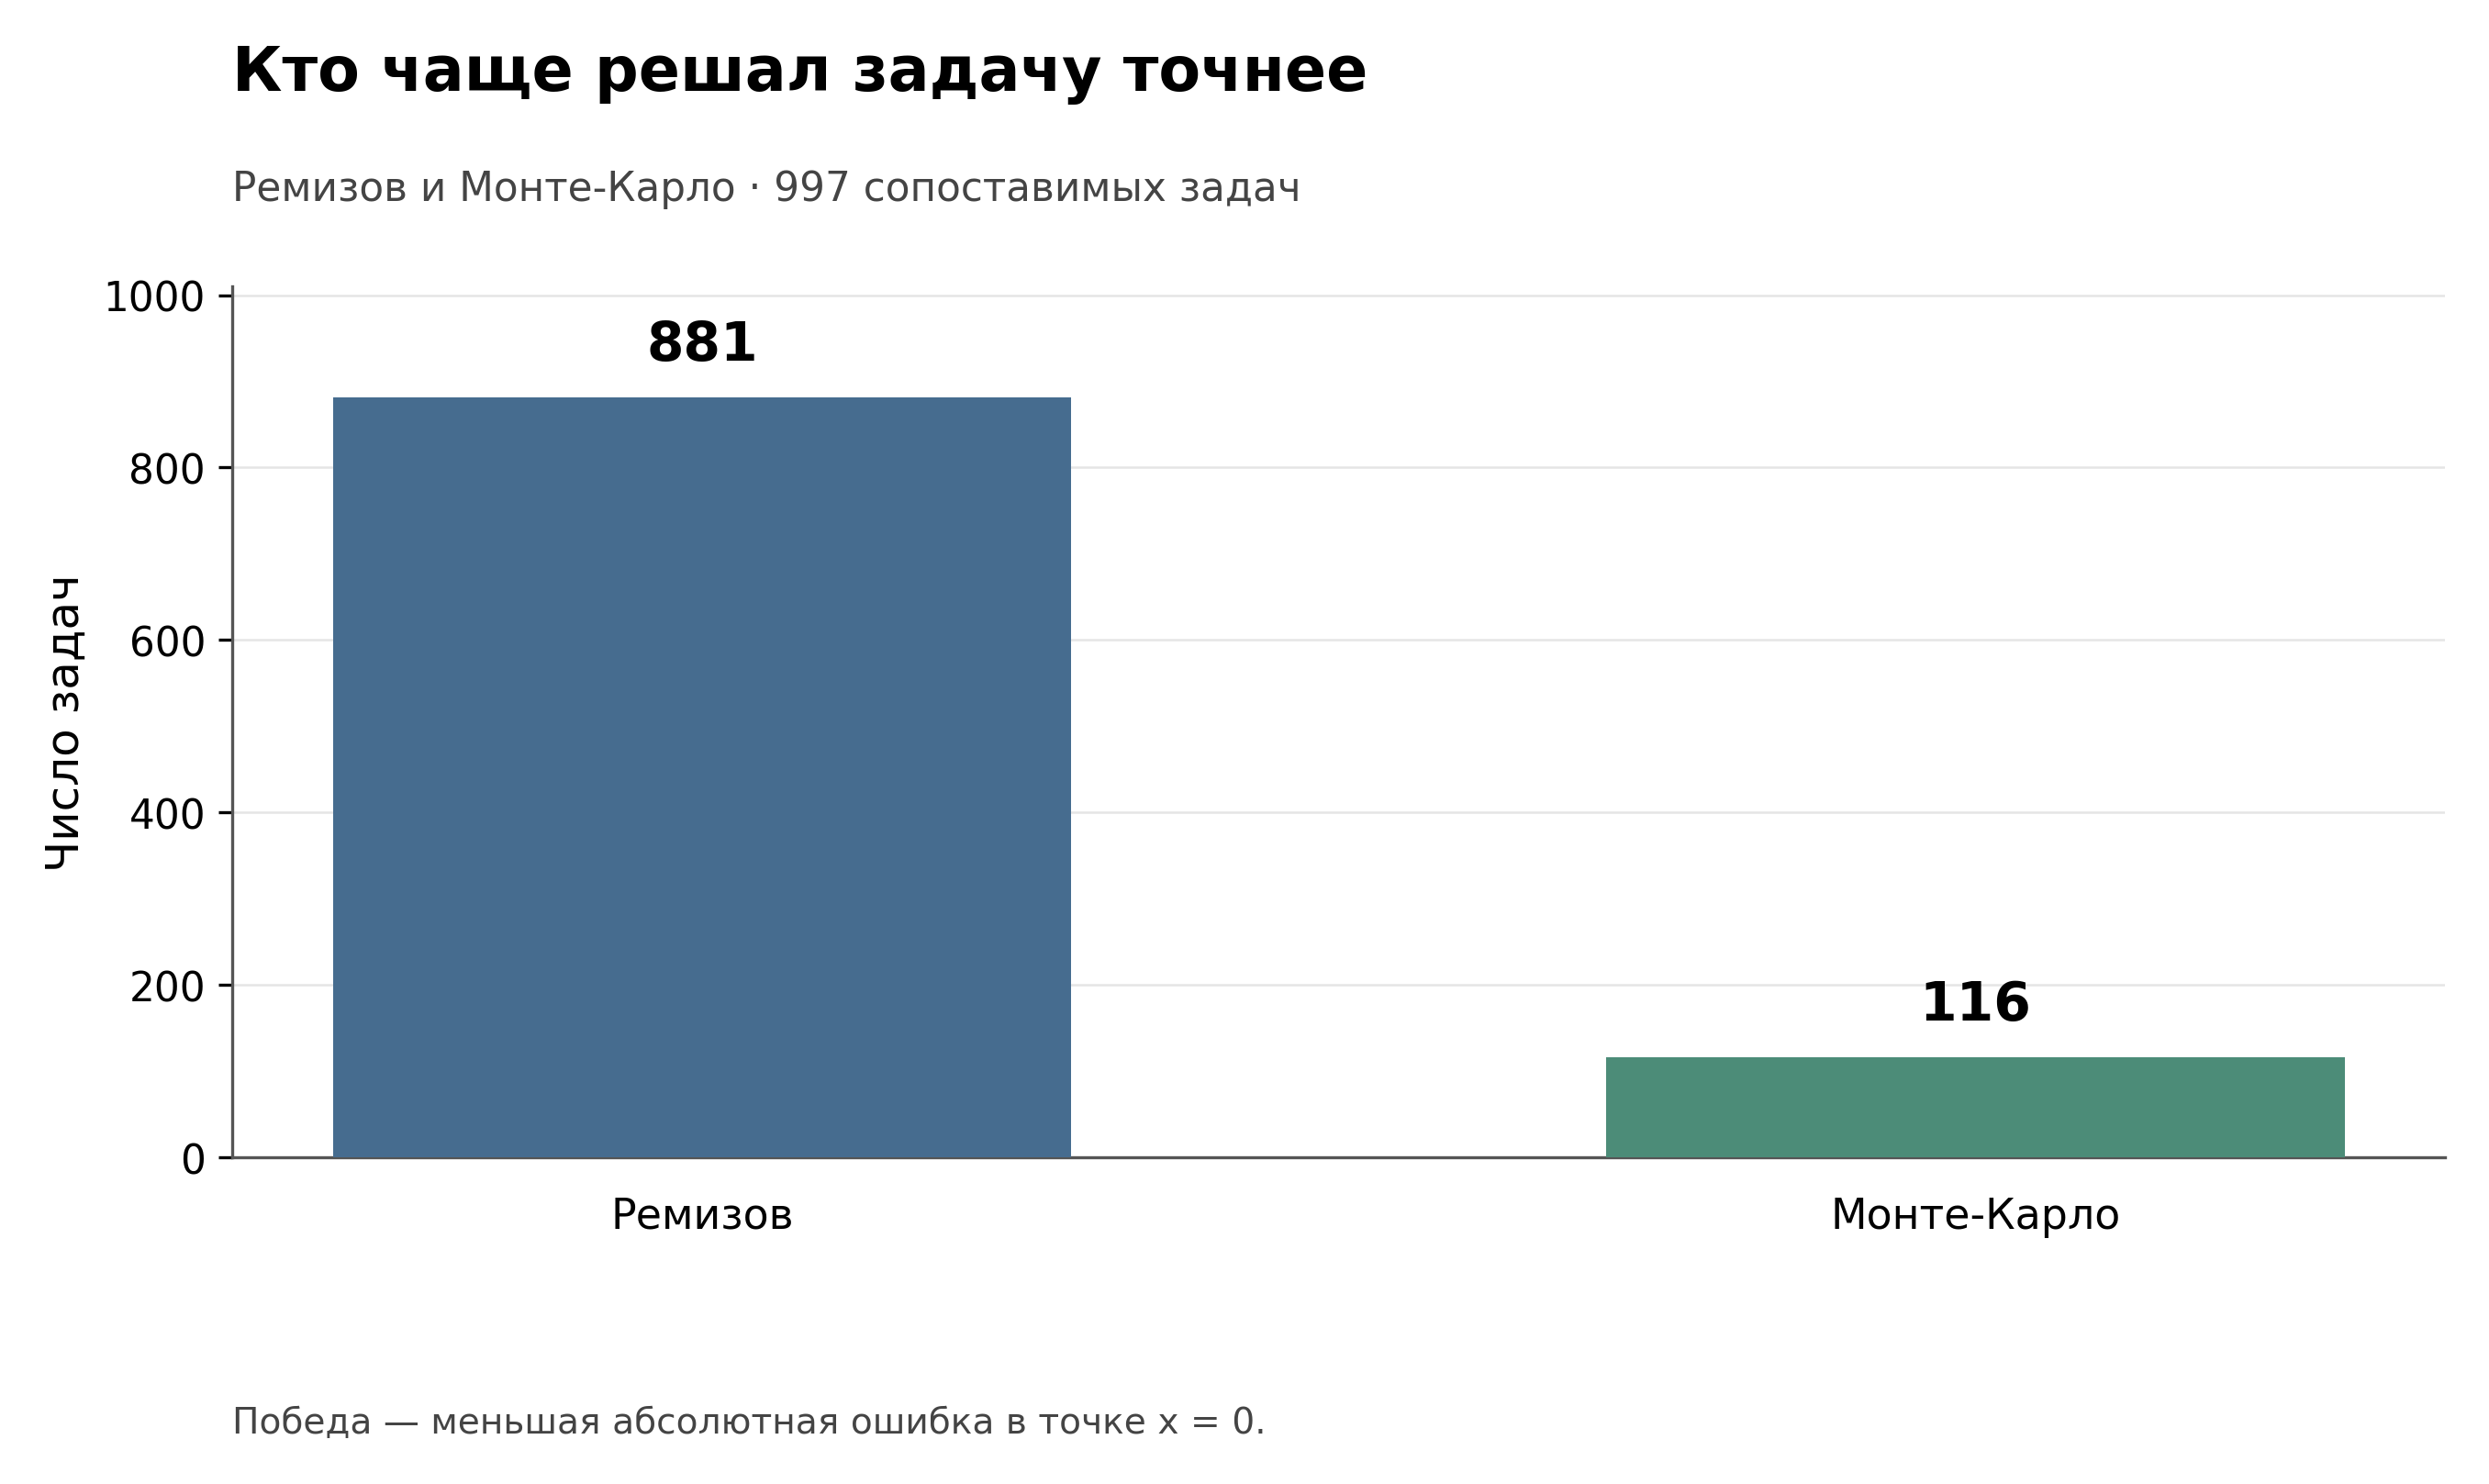
\includegraphics[width=\textwidth]{simple_01_two_methods_wins.png}
\caption{Число уравнений, на которых каждый из методов даёт меньшую
ошибку в точке $x=0$ (997 уравнений).}
\label{fig:ml-wins2}
\end{figure}

\begin{figure}[!htbp]
\centering
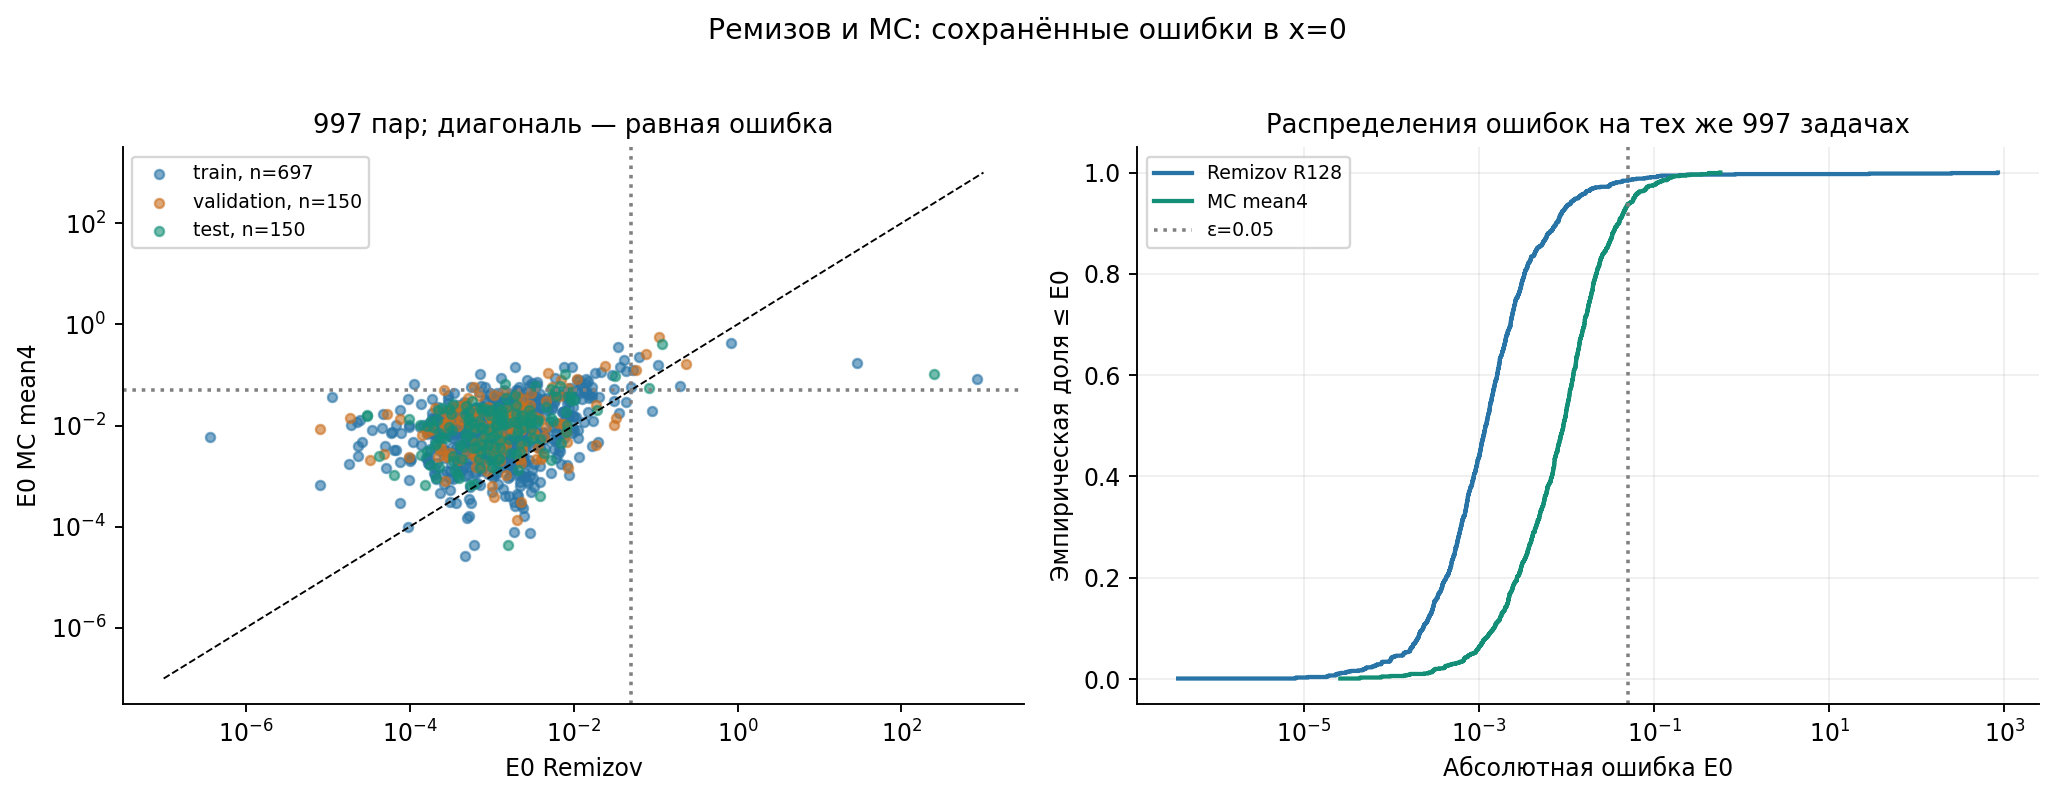
\includegraphics[width=\textwidth]{01_R_MC_error_comparison.png}
\caption{Ошибки методов Ремизова и Монте-Карло в точке $x=0$
на 997 уравнениях (логарифмические шкалы). Слева: каждая точка ---
одно уравнение; точки ниже диагонали соответствуют уравнениям, где
точнее Монте-Карло; пунктир --- уровень $0.05$. Справа: доля уравнений,
ошибка на которых не больше заданной. Remizov R128 --- метод Ремизова
при $n=128$, MC mean4 --- среднее четырёх расчётов Монте-Карло. Цвета точек
соответствуют исходному разбиению 697/150/150; в ML-эксперименте
ниже используется разбиение 747/100/150. Общий состав 997 задач одинаков.}
\label{fig:ml-errors}
\end{figure}

\subsubsection{Выбранная бинарная модель и диагностический кандидат}\label{sec:ml-res2}
Показатели диагностического кандидата CatBoost258 на трёх выборках
приведены в таблице~\ref{tab:ml-258},
его решения на тестовой выборке --- на рис.~\ref{fig:ml-test}. Показатели
на обучающей выборке вычислены на тех же данных, на которых модель
обучалась, и не являются независимой оценкой качества.

\begin{table}[!htbp]
\centering
\caption{Точечные показатели диагностического CatBoost258.
$P_{\mathrm{MC}}$ --- доля верных
среди выборов Монте-Карло, $R_{\mathrm{MC}}$ --- доля найденных уравнений,
где точнее Монте-Карло, $\bar r$ --- средняя избыточная
ошибка~\eqref{eq:ml-regret}.}
\label{tab:ml-258}
\resizebox{\textwidth}{!}{%
\begin{tabular}{lccccccc}
\toprule
Выборка & Accuracy & macro-F1 & $P_{\mathrm{MC}}$ & $R_{\mathrm{MC}}$ & средняя $E$ & $\bar r$ & $E\le0.05$\\
\midrule
Train (747) & 91.97\% & 0.803 & 0.718 & 0.596 & 0.00506 & 0.00075 & 733/747\\
Validation (100) & 89.00\% & 0.707 & 0.625 & 0.385 & 0.00347 & 0.00088 & 99/100\\
Test (150) & 88.67\% & 0.676 & 0.300 & 0.667 & 0.00560 & 0.00171 & 145/150\\
\bottomrule
\end{tabular}}
\end{table}

\begin{figure}[!htbp]
\centering
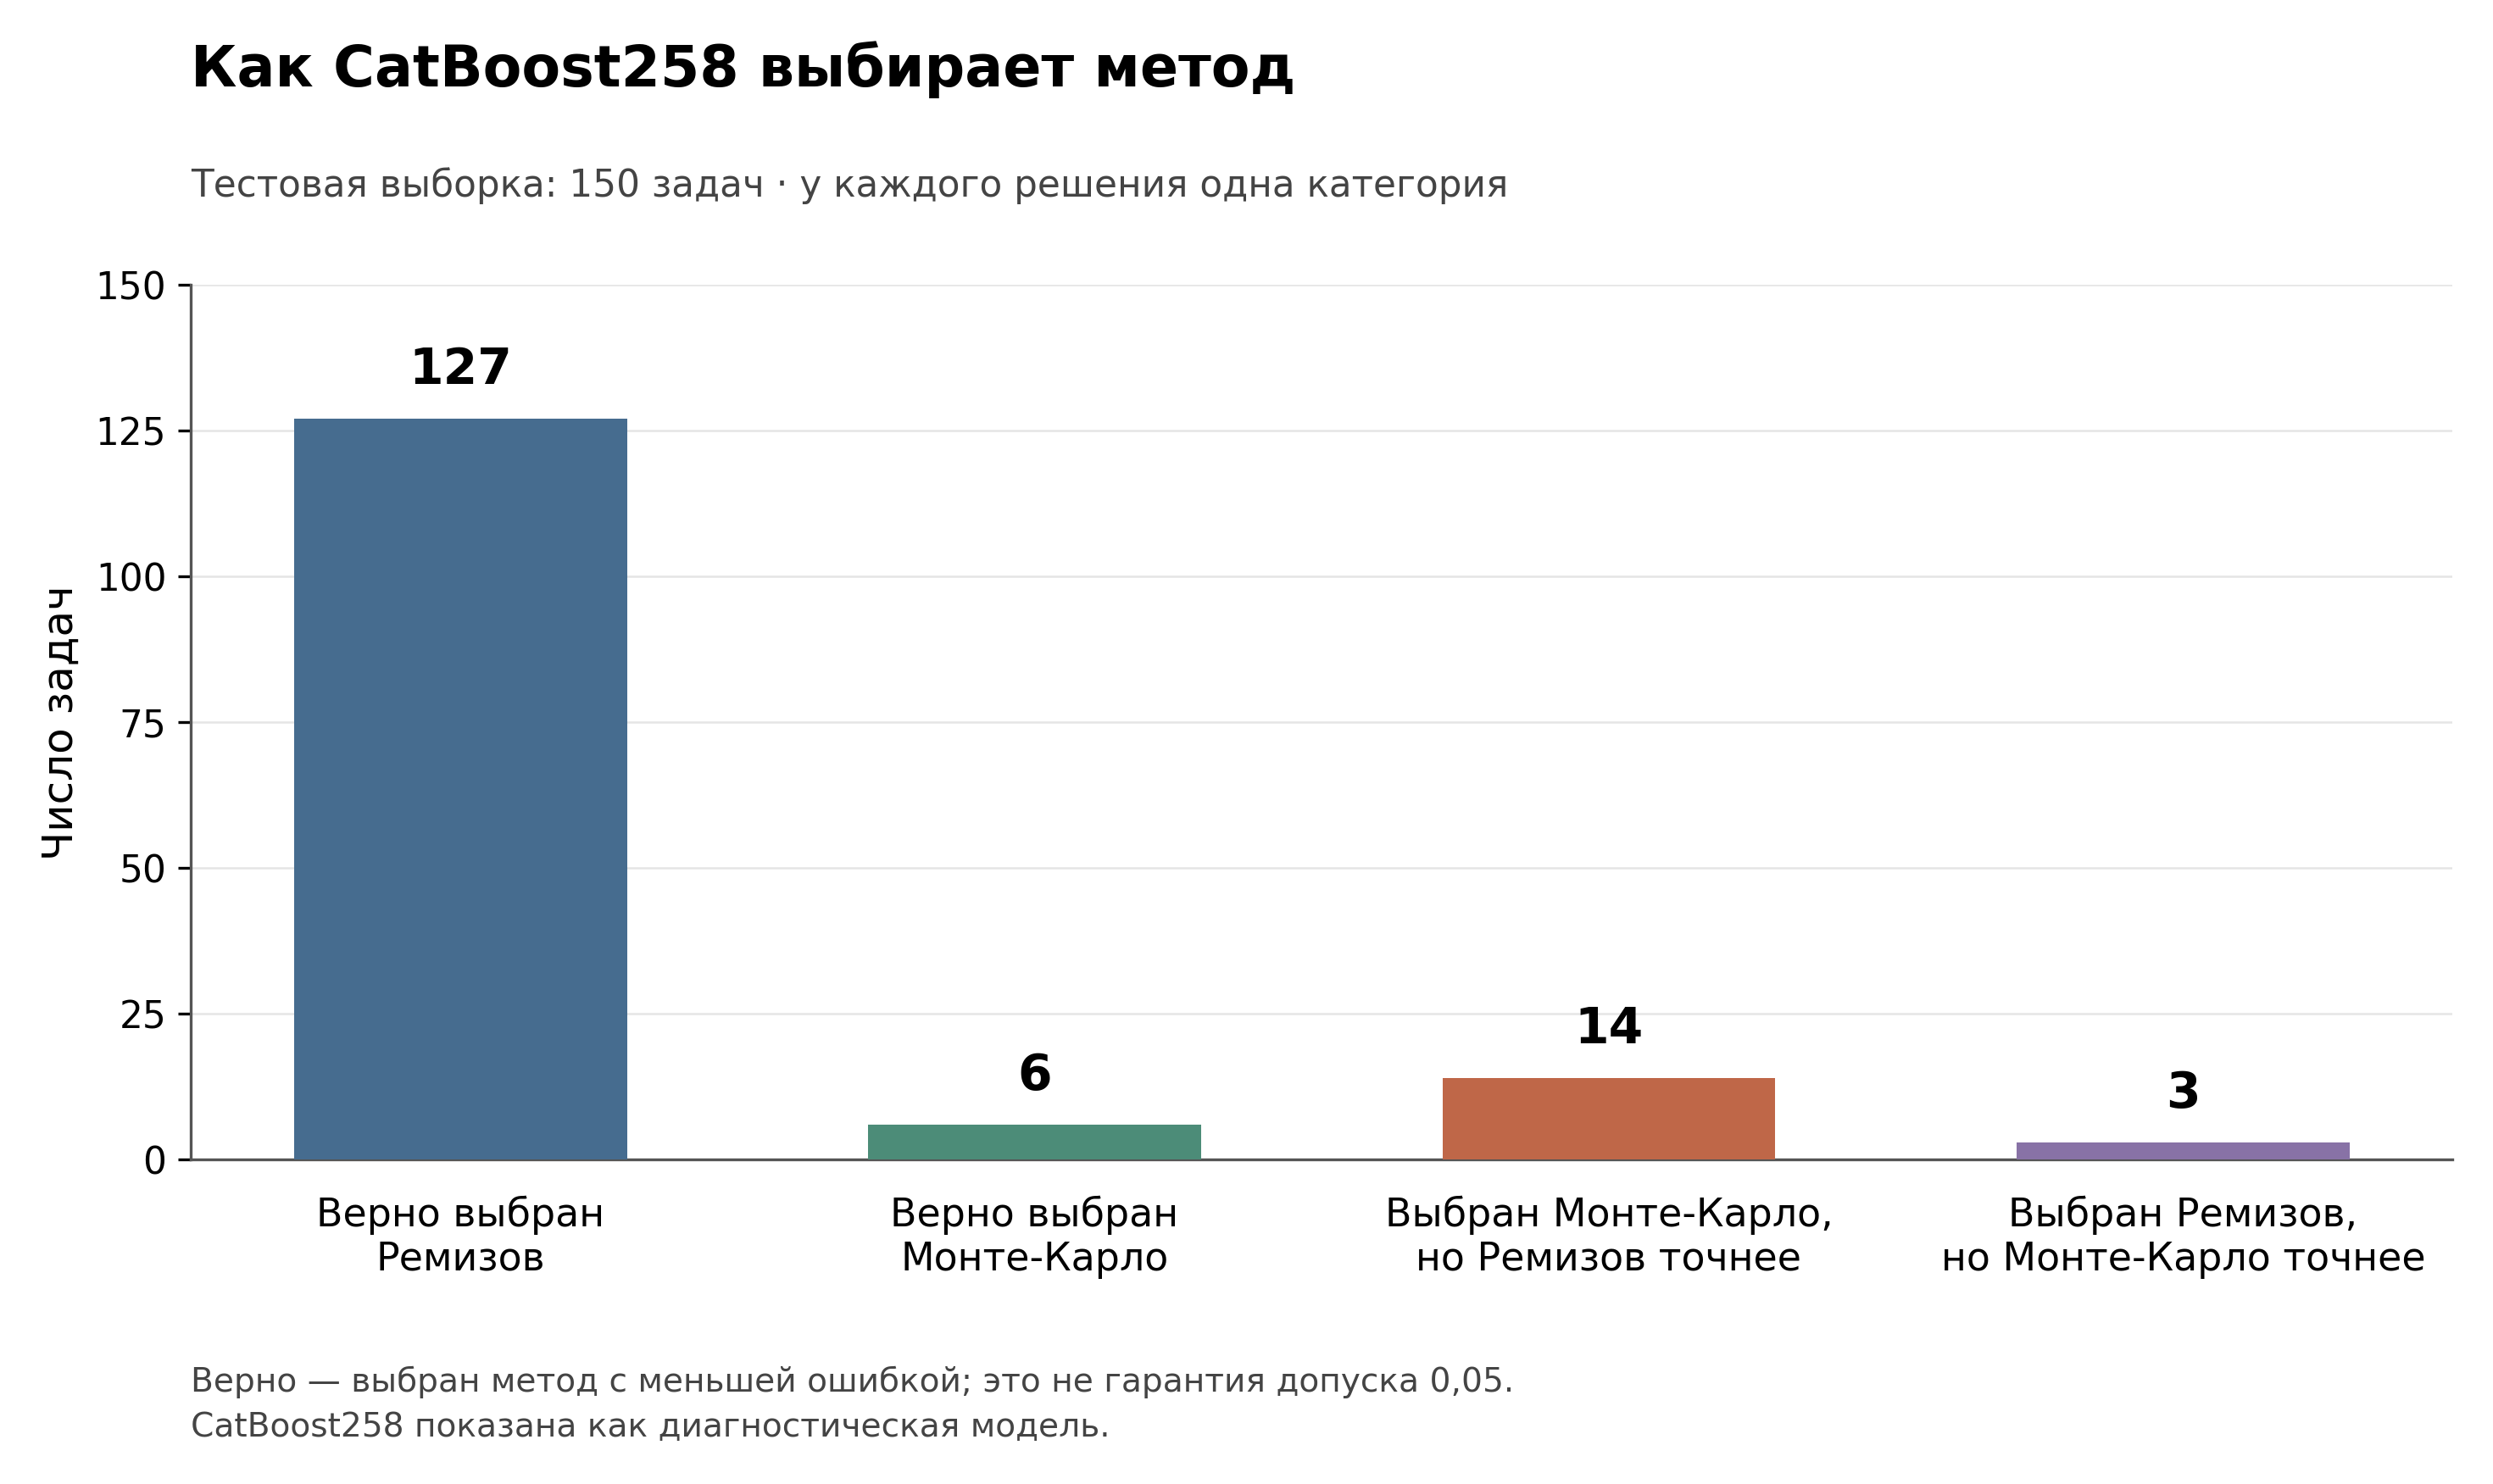
\includegraphics[width=\textwidth]{simple_02_two_methods_model_test.png}
\caption{Решения диагностического CatBoost258 на Test (150 уравнений). Верным
считается выбор метода с меньшей ошибкой; это не гарантирует достижения
точности $0.05$.}
\label{fig:ml-test}
\end{figure}

В таблице~\ref{tab:ml-rules} оба бинарных варианта сравниваются
с простыми правилами
выбора на тестовой выборке. Идеальный выбор --- выбор по известным
ошибкам; до решения уравнения он недоступен и показывает предел,
к которому можно стремиться.

\begin{table}[!htbp]
\centering
\caption{Точечные ошибки выбранной бинарной модели, диагностического
кандидата и простых правил на Test (150 уравнений).}
\label{tab:ml-rules}
\resizebox{\textwidth}{!}{%
\begin{tabular}{lcccc}
\toprule
Правило выбора & средняя $E$ & $\bar r$ & TP/FP/FN & $E\le0.05$\\
\midrule
выбранная, 253 признака & 1.65980 & 1.65590 & 1/5/8 & 146/150\\
диагностическая, 258 & 0.00560 & 0.00171 & 6/14/3 & 145/150\\
всегда метод Ремизова & 1.659 & 1.655 & 0/0/9 & 147/150\\
всегда Монте-Карло & 0.01728 & 0.01338 & 9/141/0 & 141/150\\
идеальный выбор & 0.00390 & 0 & 9/0/0 & 147/150\\
\bottomrule
\end{tabular}}
\end{table}

Выбор по Validation и итоговые точечные показатели разграничены
в таблице~\ref{tab:binary-selection}. По Validation выбрана модель
с 253 признаками: её $\bar r=0.0007103513$ меньше, чем
$0.0008760301$ у CatBoost258. На Test выбранный вариант имеет
accuracy $91.33\%$, macro-F1 $0.543860$ и не улучшает среднюю ошибку
относительно постоянного выбора метода Ремизова.

\begin{table}[!htbp]
\centering
\caption{Выбор бинарной модели по Validation; все показатели относятся к $E_m$ в нуле.}
\label{tab:binary-selection}
\resizebox{\textwidth}{!}{%
\begin{tabular}{lccccc}
\toprule
Вариант & порог & Validation $\bar r$ & Test accuracy & Test macro-F1 & Test $E\le0.05$\\
\midrule
выбранный, 253 & 0.25 & 0.0007103513 & 91.33\% & 0.543860 & 146/150\\
диагностический, 258 & 0.2006671072 & 0.0008760301 & 88.67\% & 0.675531 & 145/150\\
\bottomrule
\end{tabular}}
\end{table}

Далее подробно разбирается диагностический кандидат с 258 признаками.
Он находит 6 из 9 уравнений, где точнее Монте-Карло, но лишь 30\%
его выборов Монте-Карло верны: из 20 таких выборов ошибочны 14. Число
уравнений, на которых достигнута точность $0.05$, уменьшается со 147
при постоянном выборе метода Ремизова до 145.

Большая разница средних ошибок модели и постоянного выбора метода
Ремизова требует оговорки. Она почти целиком определяется одним
уравнением \texttt{AMV1\_F0180\_S04}, где $E_{\mathrm{R}}=248.3$,
а $E_{\mathrm{MC}}=0.103$: при выборе метода Ремизова избыточная ошибка
на нём равна $248.2$, что после деления на 150 даёт $1.655$. Модель верно
выбирает на этом уравнении Монте-Карло, но точность $0.05$ всё равно
не достигнута. Если для проверки устойчивости вывода исключить это
уравнение, то на остальных 149 средняя ошибка постоянного выбора метода
Ремизова равна $0.00350$, а модели --- $0.00495$, то есть преимущество
меняет знак. Во всех основных результатах это уравнение сохранено.
Насколько результат переносится на другие семейства уравнений,
не установлено.

\subsubsection{Разбор неверных выборов диагностического кандидата}
На тестовой выборке диагностический CatBoost258 ошибся 17 раз:
14 раз выбрал Монте-Карло, когда точнее метод Ремизова (FP),
и 3 раза выбрал метод Ремизова, когда
точнее Монте-Карло (FN). Все случаи приведены
в таблице~\ref{tab:ml-wrong} и на рис.~\ref{fig:ml-wrong}; для каждого
из них избыточная ошибка равна $|\Delta|=|E_{\mathrm{R}}-E_{\mathrm{MC}}|$.

\begin{table}[!htbp]
\centering
\caption{Неверные выборы диагностического CatBoost258 на Test по ошибке в нуле.
$\Delta=E_{\mathrm{R}}-E_{\mathrm{MC}}$; отрицательное значение означает,
что точнее метод Ремизова. Значения округлены.}
\label{tab:ml-wrong}
\resizebox{\textwidth}{!}{%
\begin{tabular}{llcccl}
\toprule
Уравнение & Тип & $E_{\mathrm{R}}$ & $E_{\mathrm{MC}}$ & $\Delta$ & Точность $0.05$\\
\midrule
\texttt{AMV1\_F0036\_S03} & FP & 0.001272 & 0.003581 & $-0.002310$ & у обоих методов\\
\texttt{AMV1\_F0084\_S00} & FP & 0.005260 & 0.01419 & $-0.008927$ & у обоих методов\\
\texttt{AMV1\_F0084\_S03} & FP & 0.005535 & 0.01253 & $-0.006993$ & у обоих методов\\
\texttt{AMV1\_F0094\_S01} & FP & 0.0007748 & 0.02212 & $-0.02134$ & у обоих методов\\
\texttt{AMV1\_F0098\_S02} & FP & 0.0008599 & 0.003362 & $-0.002502$ & у обоих методов\\
\texttt{AMV1\_F0098\_S04} & FP & 0.001981 & 0.01702 & $-0.01504$ & у обоих методов\\
\texttt{AMV1\_F0100\_S04} & FP & 0.0004919 & 0.006008 & $-0.005516$ & у обоих методов\\
\texttt{AMV1\_F0164\_S01} & FP & 0.0002026 & 0.004107 & $-0.003904$ & у обоих методов\\
\texttt{AMV1\_F0179\_S03} & FP & 0.008291 & 0.01010 & $-0.001805$ & у обоих методов\\
\texttt{AMV1\_F0180\_S01} & FP & 0.03175 & 0.09655 & $-0.06480$ & \textbf{теряется}\\
\texttt{AMV1\_F0180\_S02} & FP & 0.003379 & 0.06041 & $-0.05704$ & \textbf{теряется}\\
\texttt{AMV1\_F0190\_S01} & FP & 0.009266 & 0.04533 & $-0.03606$ & у обоих методов\\
\texttt{AMV1\_F0191\_S03} & FP & 0.001227 & 0.002277 & $-0.001050$ & у обоих методов\\
\texttt{AMV1\_F0191\_S04} & FP & 0.01014 & 0.03150 & $-0.02136$ & у обоих методов\\
\texttt{AMV1\_F0070\_S02} & FN & 0.002124 & 0.001312 & $0.0008121$ & у обоих методов\\
\texttt{AMV1\_F0190\_S04} & FN & 0.003905 & 0.0004051 & $0.003500$ & у обоих методов\\
\texttt{AMV1\_F0191\_S01} & FN & 0.005347 & 0.002114 & $0.003233$ & у обоих методов\\
\bottomrule
\end{tabular}}
\end{table}

\begin{figure}[!htbp]
\centering
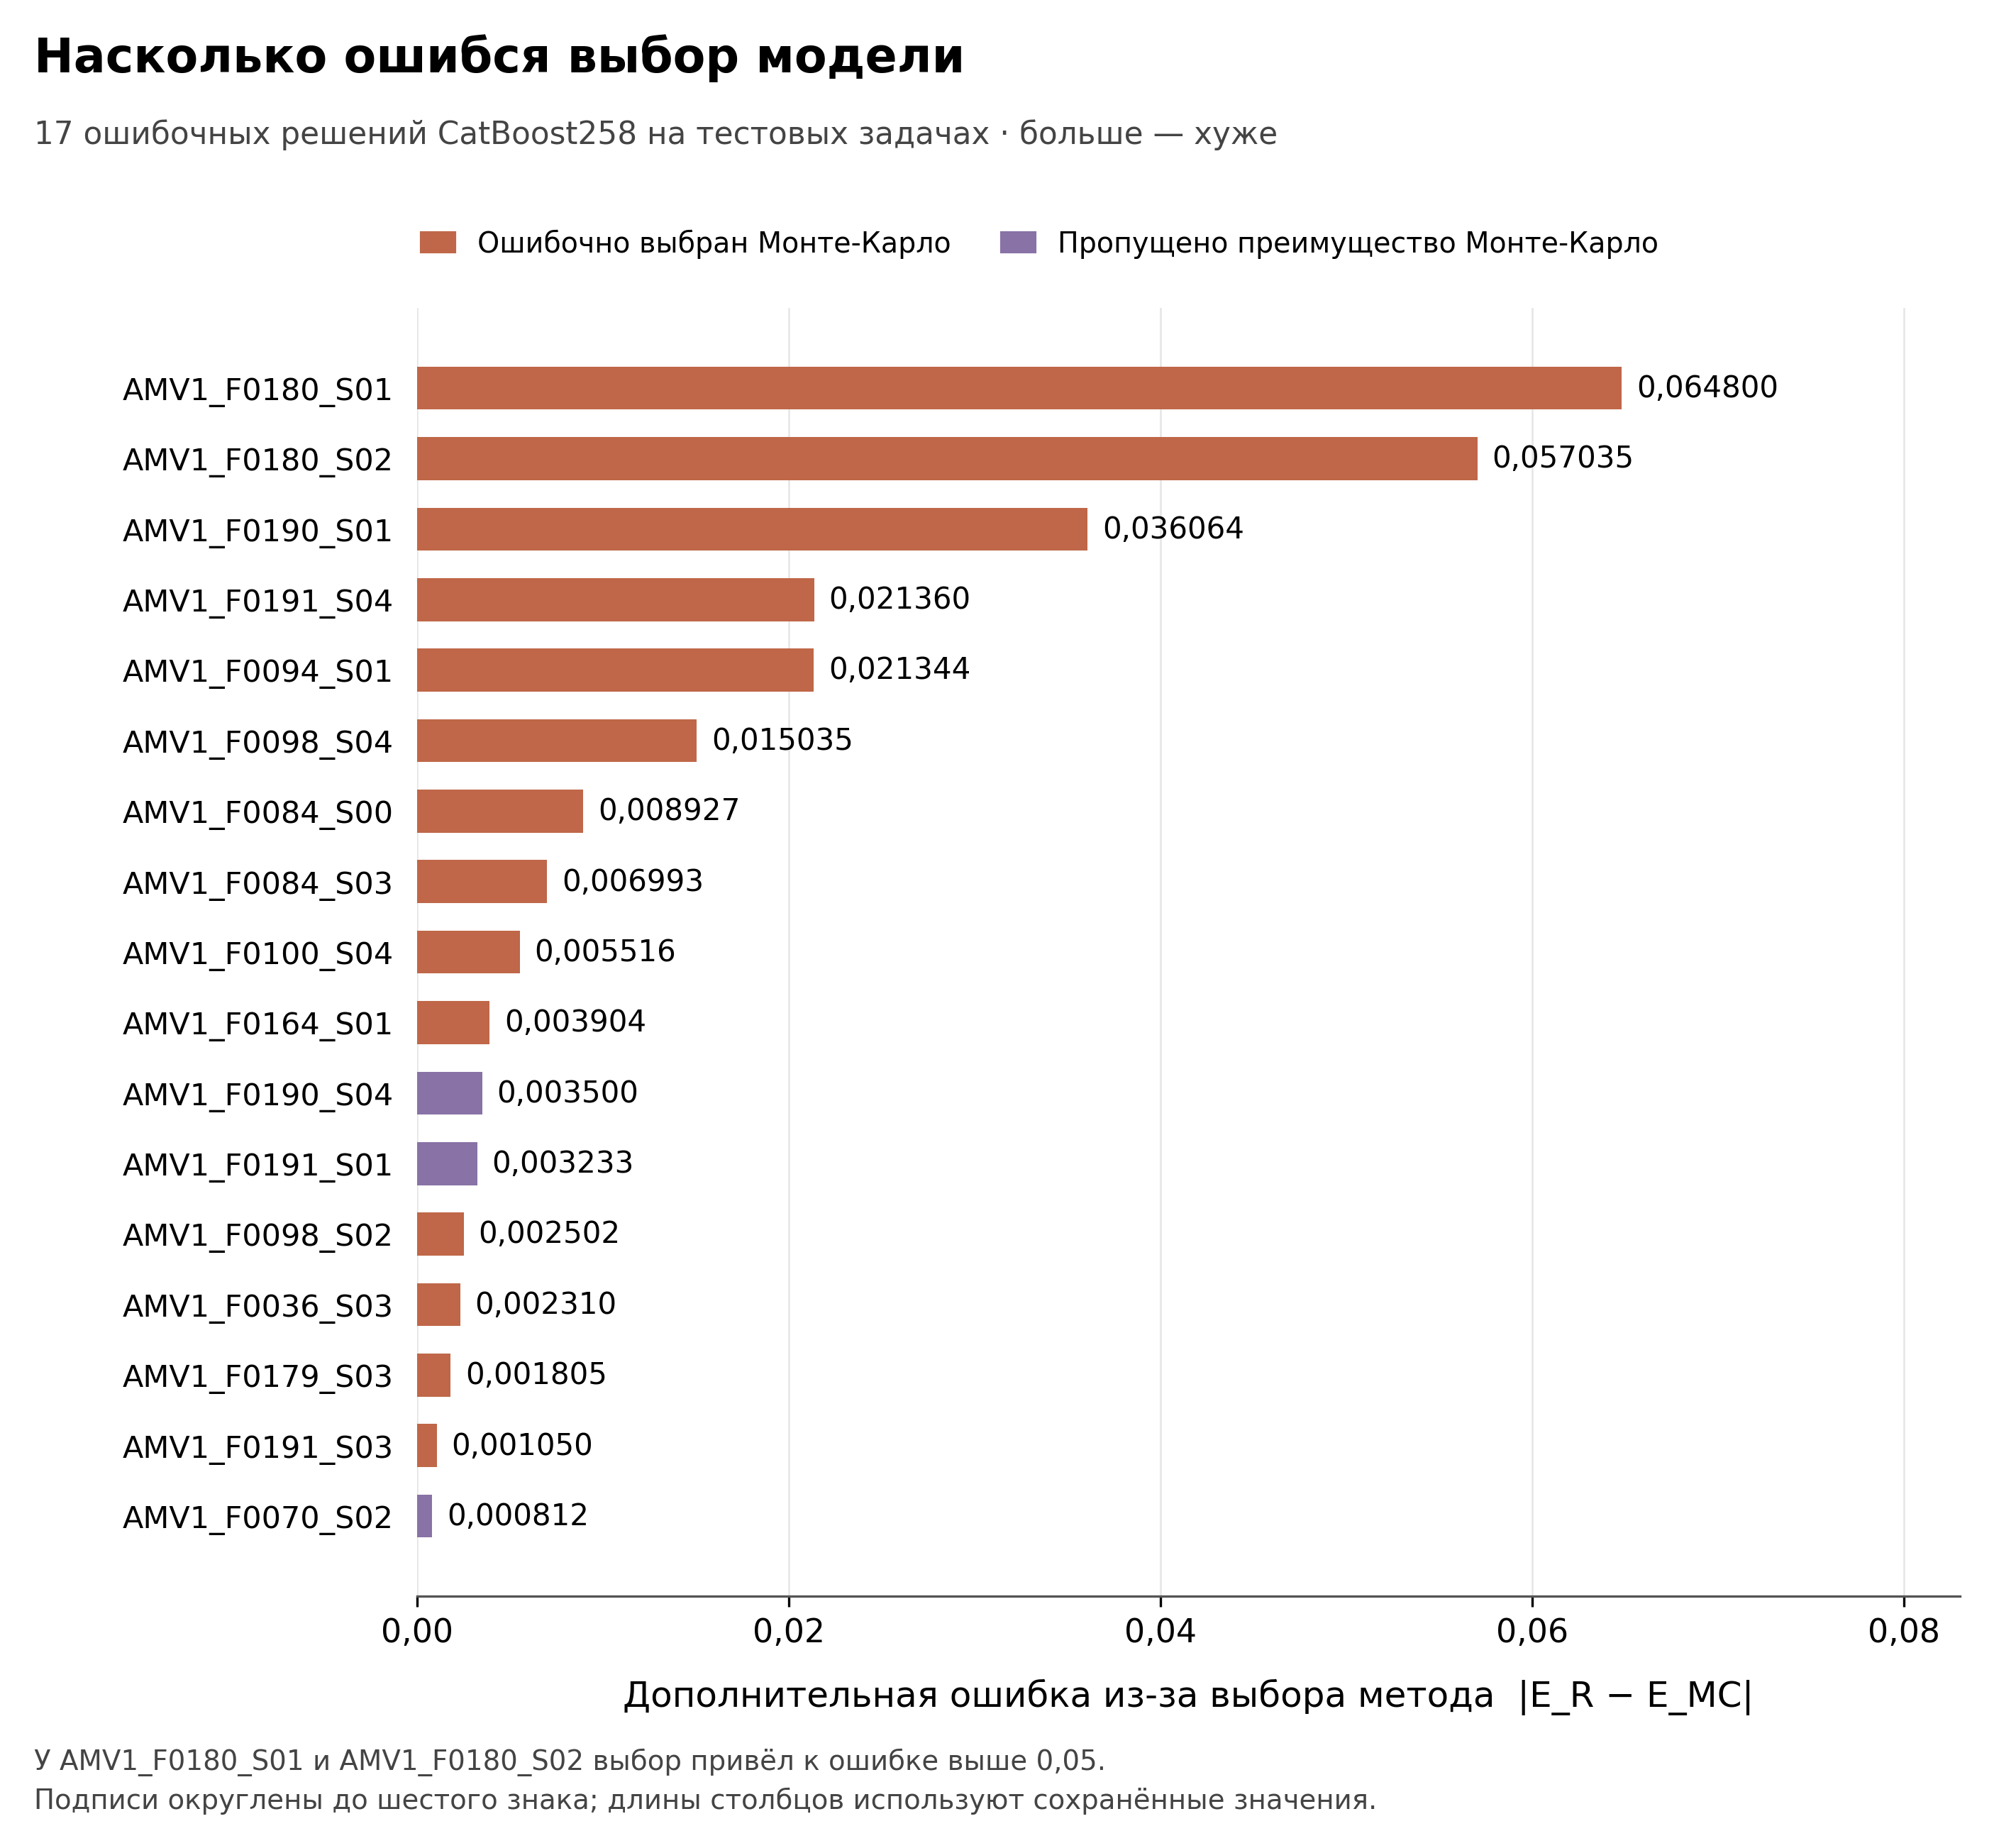
\includegraphics[width=0.85\textwidth]{simple_03_wrong_mc_choices.png}
\caption{Избыточная ошибка $|E_{\mathrm{R}}-E_{\mathrm{MC}}|$
в 17 неверных выборах диагностического CatBoost258; цвет показывает тип ошибки.}
\label{fig:ml-wrong}
\end{figure}

В 12 из 14 случаев FP оба метода достигают точности $0.05$, но разница
ошибок не всегда мала. Например, для \texttt{AMV1\_F0190\_S01} ошибка
возрастает с $0.0093$ до $0.0453$, почти до порога. В двух случаях
неверный выбор приводит к потере точности: для \texttt{AMV1\_F0180\_S01}
ошибка возрастает с $0.0317$ до $0.0965$, для \texttt{AMV1\_F0180\_S02}
--- с $0.0034$ до $0.0604$; избыточные ошибки равны $0.0648$ и $0.0570$.

Во всех трёх случаях FN оба метода достигают точности $0.05$;
упущенное уменьшение ошибки лежит между $0.0008$ и $0.0035$. Суммарная
избыточная ошибка 14 случаев FP равна $0.2486$, трёх случаев FN ---
$0.0075$; вместе $0.2562$, что даёт $\bar r=0.00171$ на 150 уравнениях.
Ни в одном случае модель не заменила метод Ремизова, не достигающий
точности, на Монте-Карло, достигающий её. На двух уравнениях, где модель
верно выбрала Монте-Карло, \texttt{AMV1\_F0070\_S04}
и \texttt{AMV1\_F0180\_S04}, ошибки равны $0.0563$ и $0.1031$, то есть
обе больше $0.05$. Таким образом, умение выбрать более точный метод
и достижение требуемой точности --- разные свойства.

\subsubsection{Сравнение четырёх методов}
К результатам методов Ремизова и Монте-Карло добавлены результаты одного
расчёта методами RK4 и мультипликативного интеграла с настройками
из таблицы~\ref{tab:ml-settings}. Ошибки в точке $x=0$ на общих
997 уравнениях приведены в таблице~\ref{tab:ml-four}.

\begin{table}[!htbp]
\centering
\caption{Ошибки $E$ в точке $x=0$ на 997 уравнениях. Квантиль $0.95$ ---
значение, которое не превышают ошибки 95\% уравнений.}
\label{tab:ml-four}
\resizebox{\textwidth}{!}{%
\begin{tabular}{>{\raggedright\arraybackslash}p{4.8cm}ccccc}
\toprule
Метод & средняя $E$ & медиана & \begin{tabular}[b]{@{}c@{}}квантиль\\$0.95$\end{tabular} & максимум & $E\le0.05$\\
\midrule
Метод Ремизова & 1.127 & 0.00119 & 0.0135 & 842.1 & 982/997\\
Монте-Карло & 0.0181 & 0.00919 & 0.0583 & 0.570 & 935/997\\
RK4 & $1.79\cdot10^{-7}$ & $6.24\cdot10^{-9}$ & $3.89\cdot10^{-7}$ & $4.59\cdot10^{-5}$ & 997/997\\
Мультипликативный интеграл & 0.0456 & 0.0174 & 0.163 & 1.985 & 758/997\\
\bottomrule
\end{tabular}}
\end{table}

На всех 997 уравнениях наименьшую ошибку даёт RK4, совпадений ошибок нет
(рис.~\ref{fig:ml-wins4}); по уровням сложности L1--L4 это 250, 250, 247
и 250 уравнений. Если брать все уравнения, для которых есть результат
метода, то RK4 достигает точности $0.05$ на 1000 из 1000, Монте-Карло ---
на 938 из 1000, метод мультипликативного интеграла --- на 760 из 1000,
метод Ремизова --- на 982 из 997. Знаменатели здесь разные, поэтому
методы попарно сравниваются только по таблице~\ref{tab:ml-four}.

\begin{figure}[!htbp]
\centering
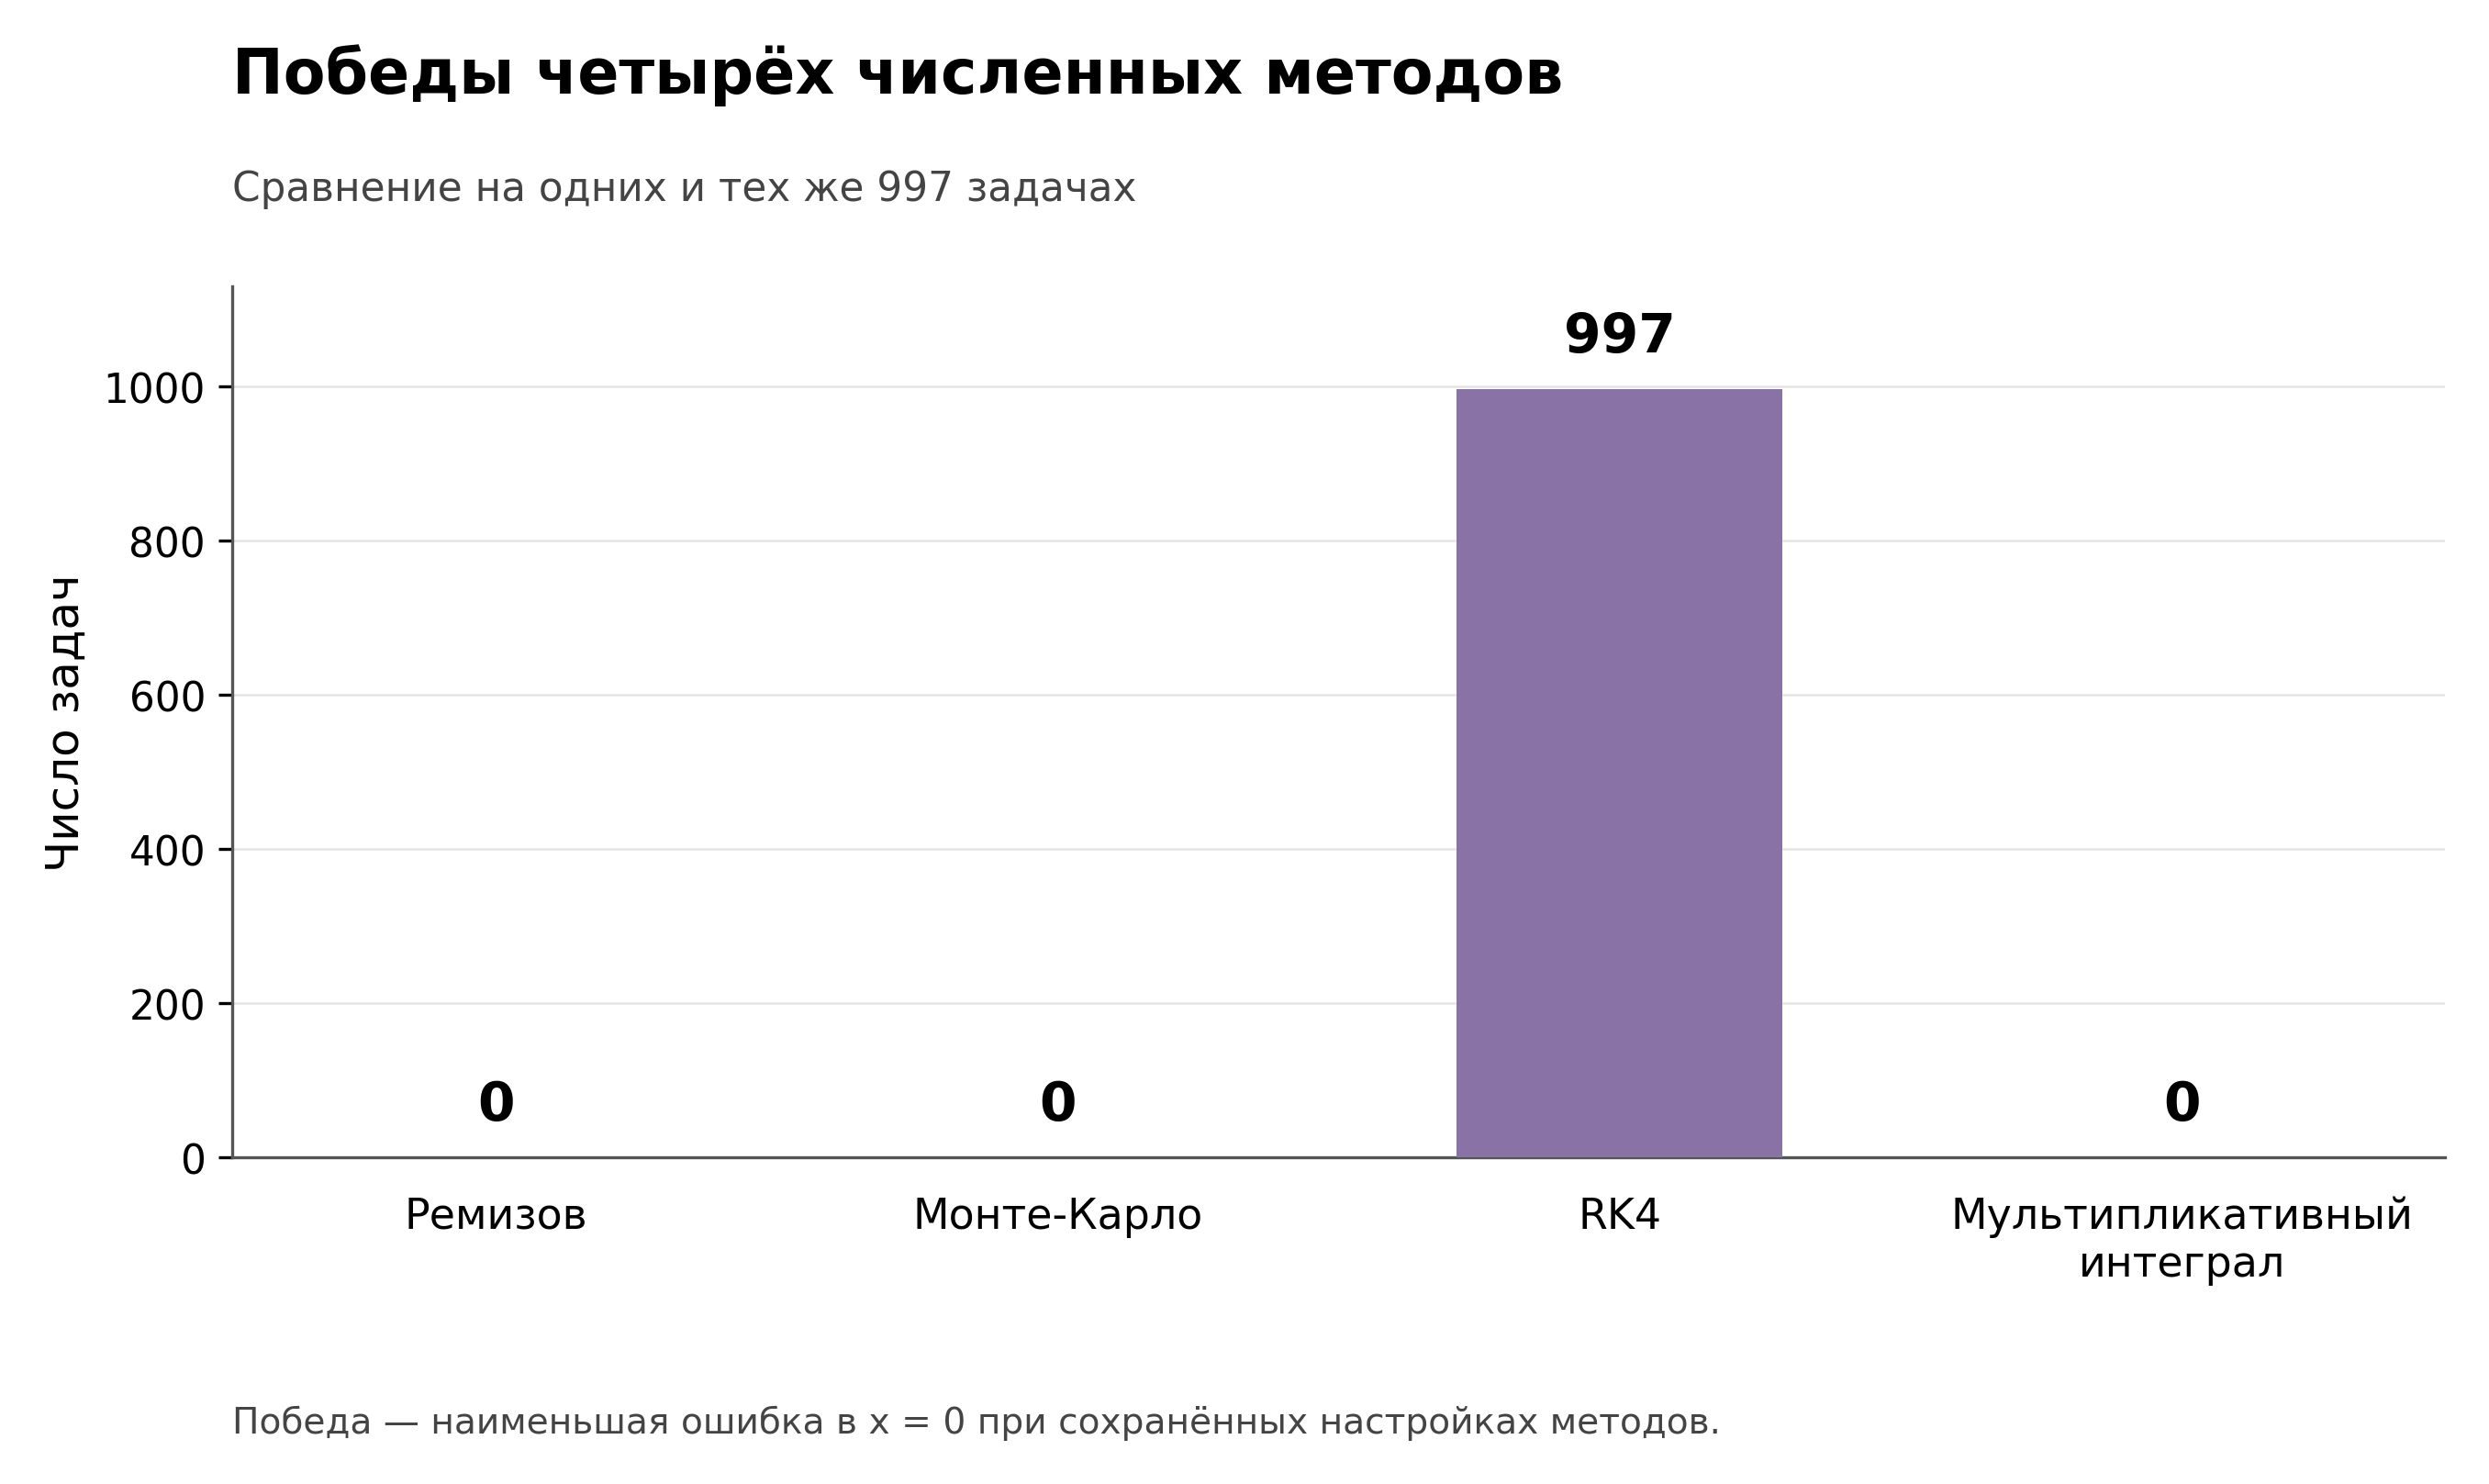
\includegraphics[width=\textwidth]{simple_04_four_methods_wins.png}
\caption{Число уравнений, на которых каждый из четырёх методов даёт
наименьшую ошибку в точке $x=0$ (997 уравнений).}
\label{fig:ml-wins4}
\end{figure}

Средние ошибки показаны на рис.~\ref{fig:ml-mean4}. Редкие очень большие
ошибки метода Ремизова сильно увеличивают его среднее, поэтому
при сравнении нужно смотреть и на медиану в таблице~\ref{tab:ml-four}.
Число уравнений, на которых каждый метод достигает точности $0.05$,
показано на рис.~\ref{fig:ml-success4}.

\begin{figure}[!htbp]
\centering
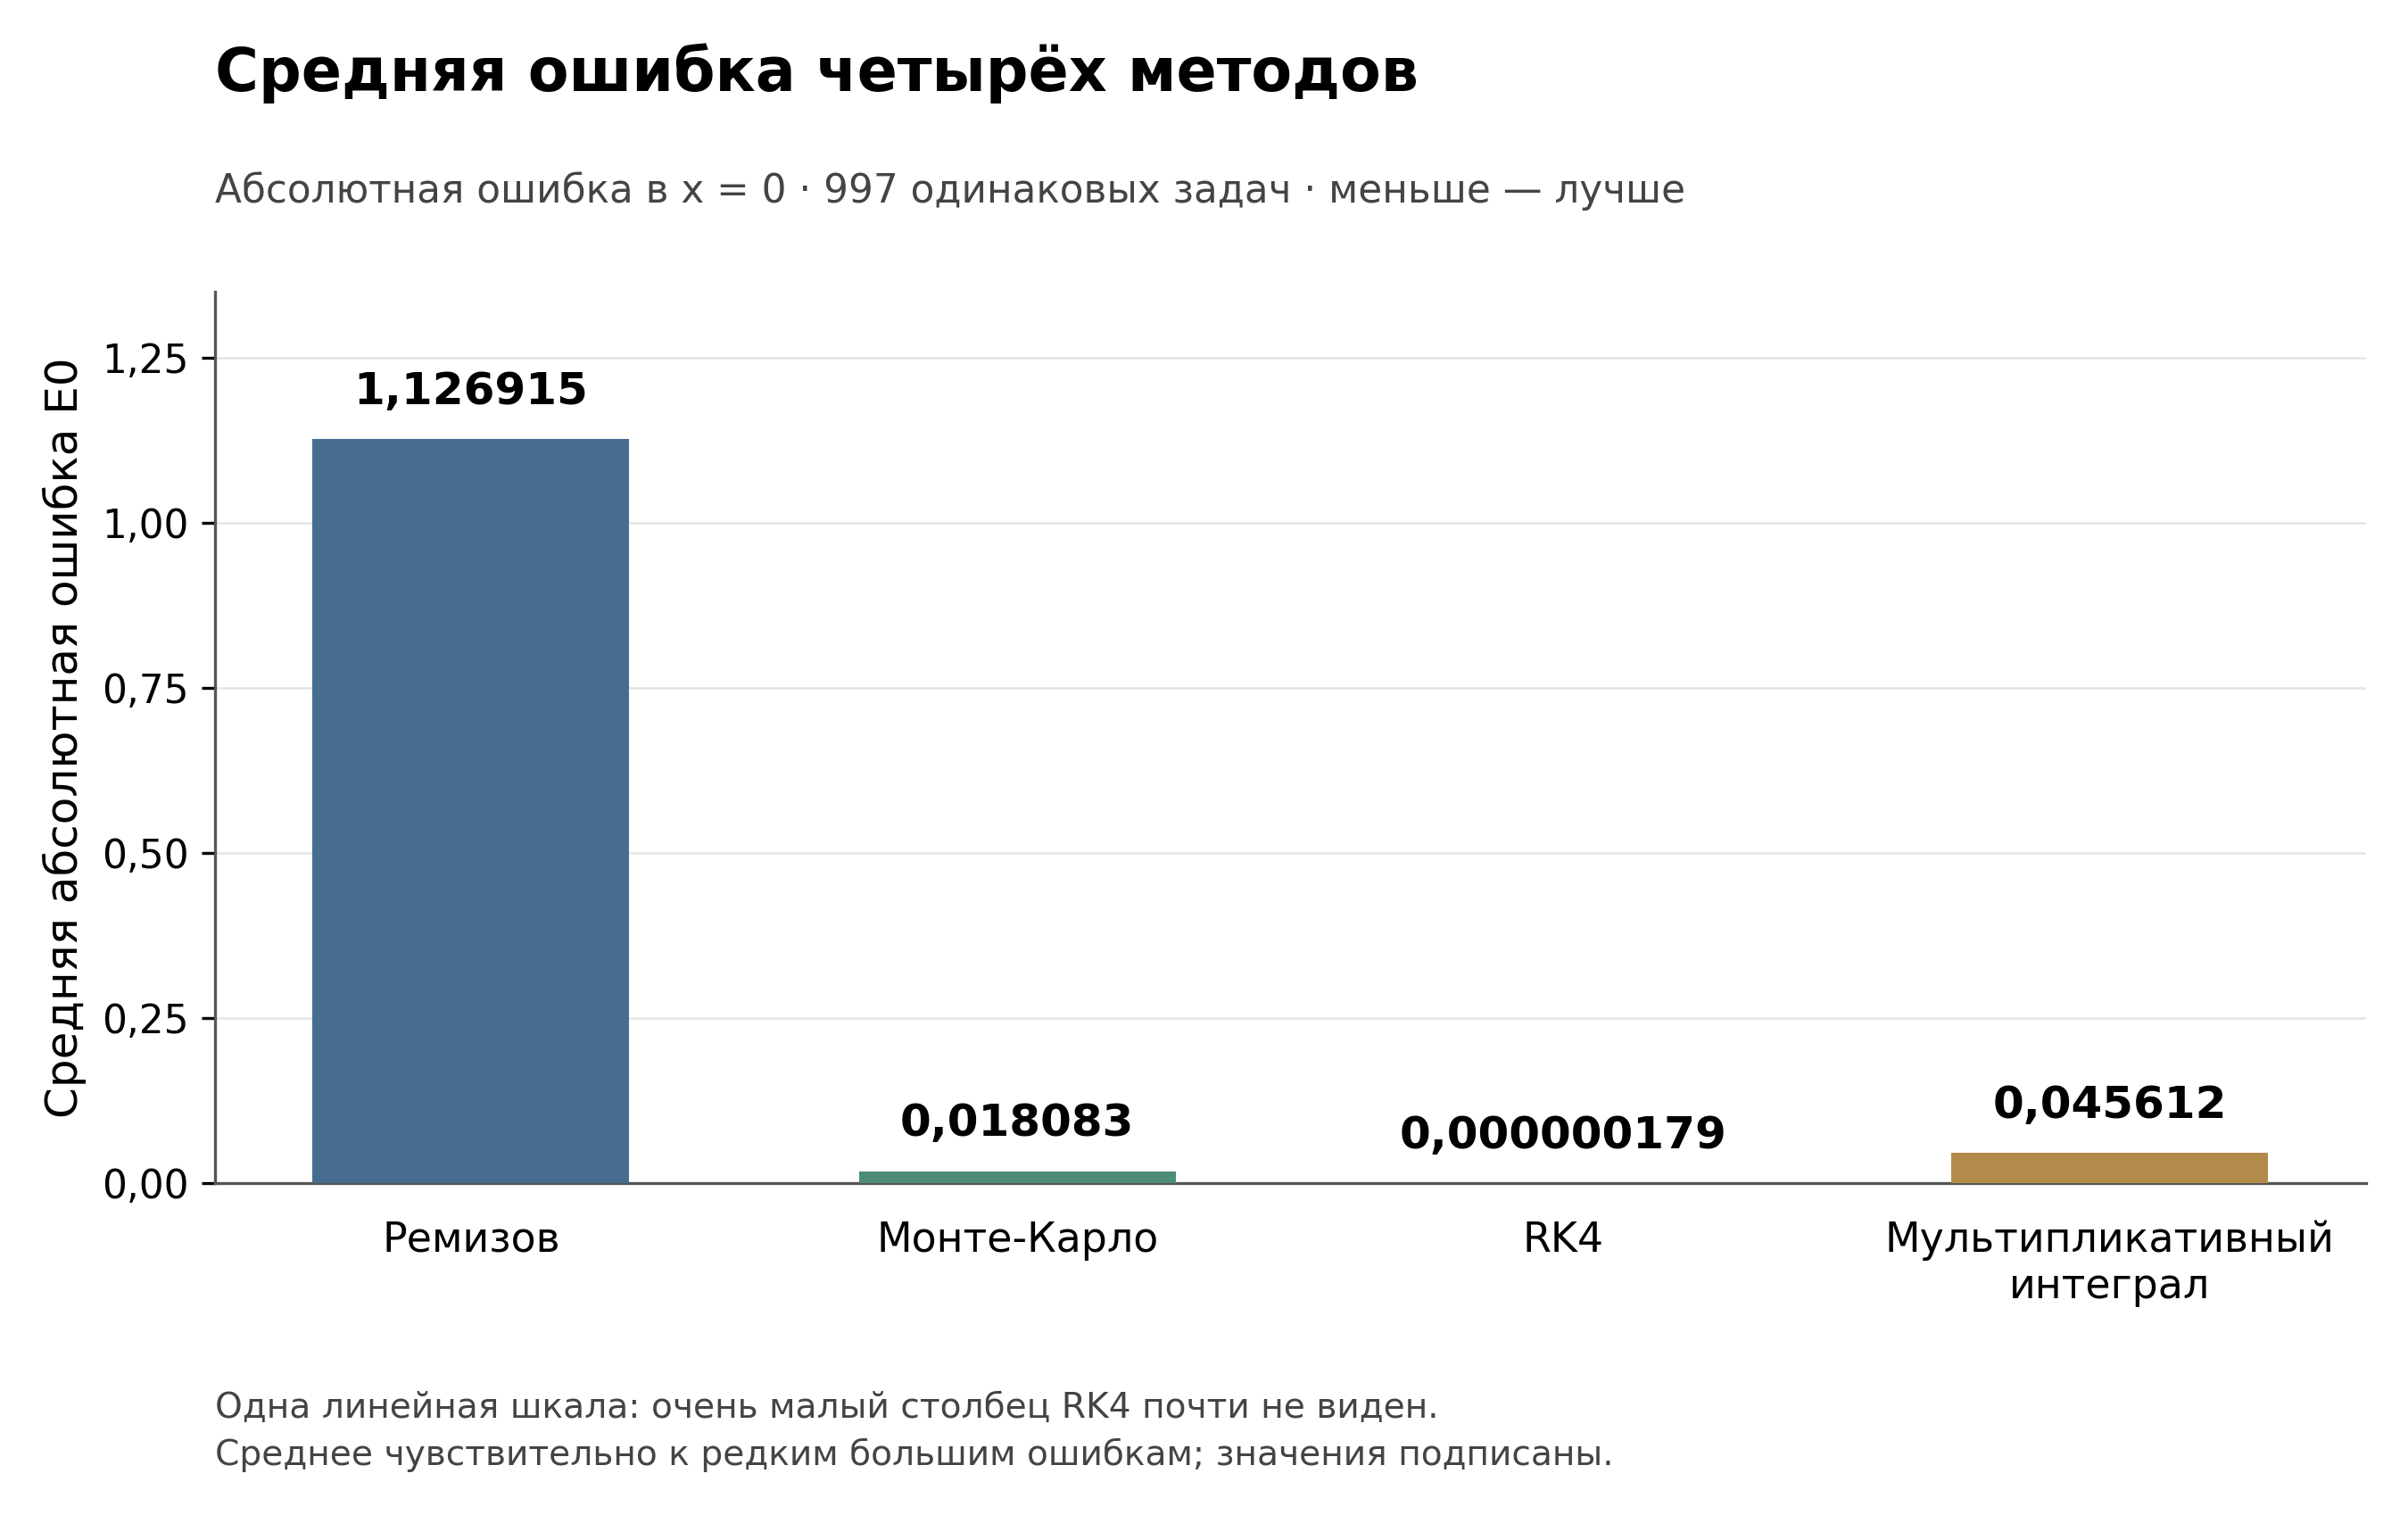
\includegraphics[width=\textwidth]{simple_05_four_methods_mean_error.png}
\caption{Средняя ошибка четырёх методов в точке $x=0$ на 997 уравнениях.
Шкала линейная, поэтому столбец RK4 почти не виден.}
\label{fig:ml-mean4}
\end{figure}

\begin{figure}[!htbp]
\centering
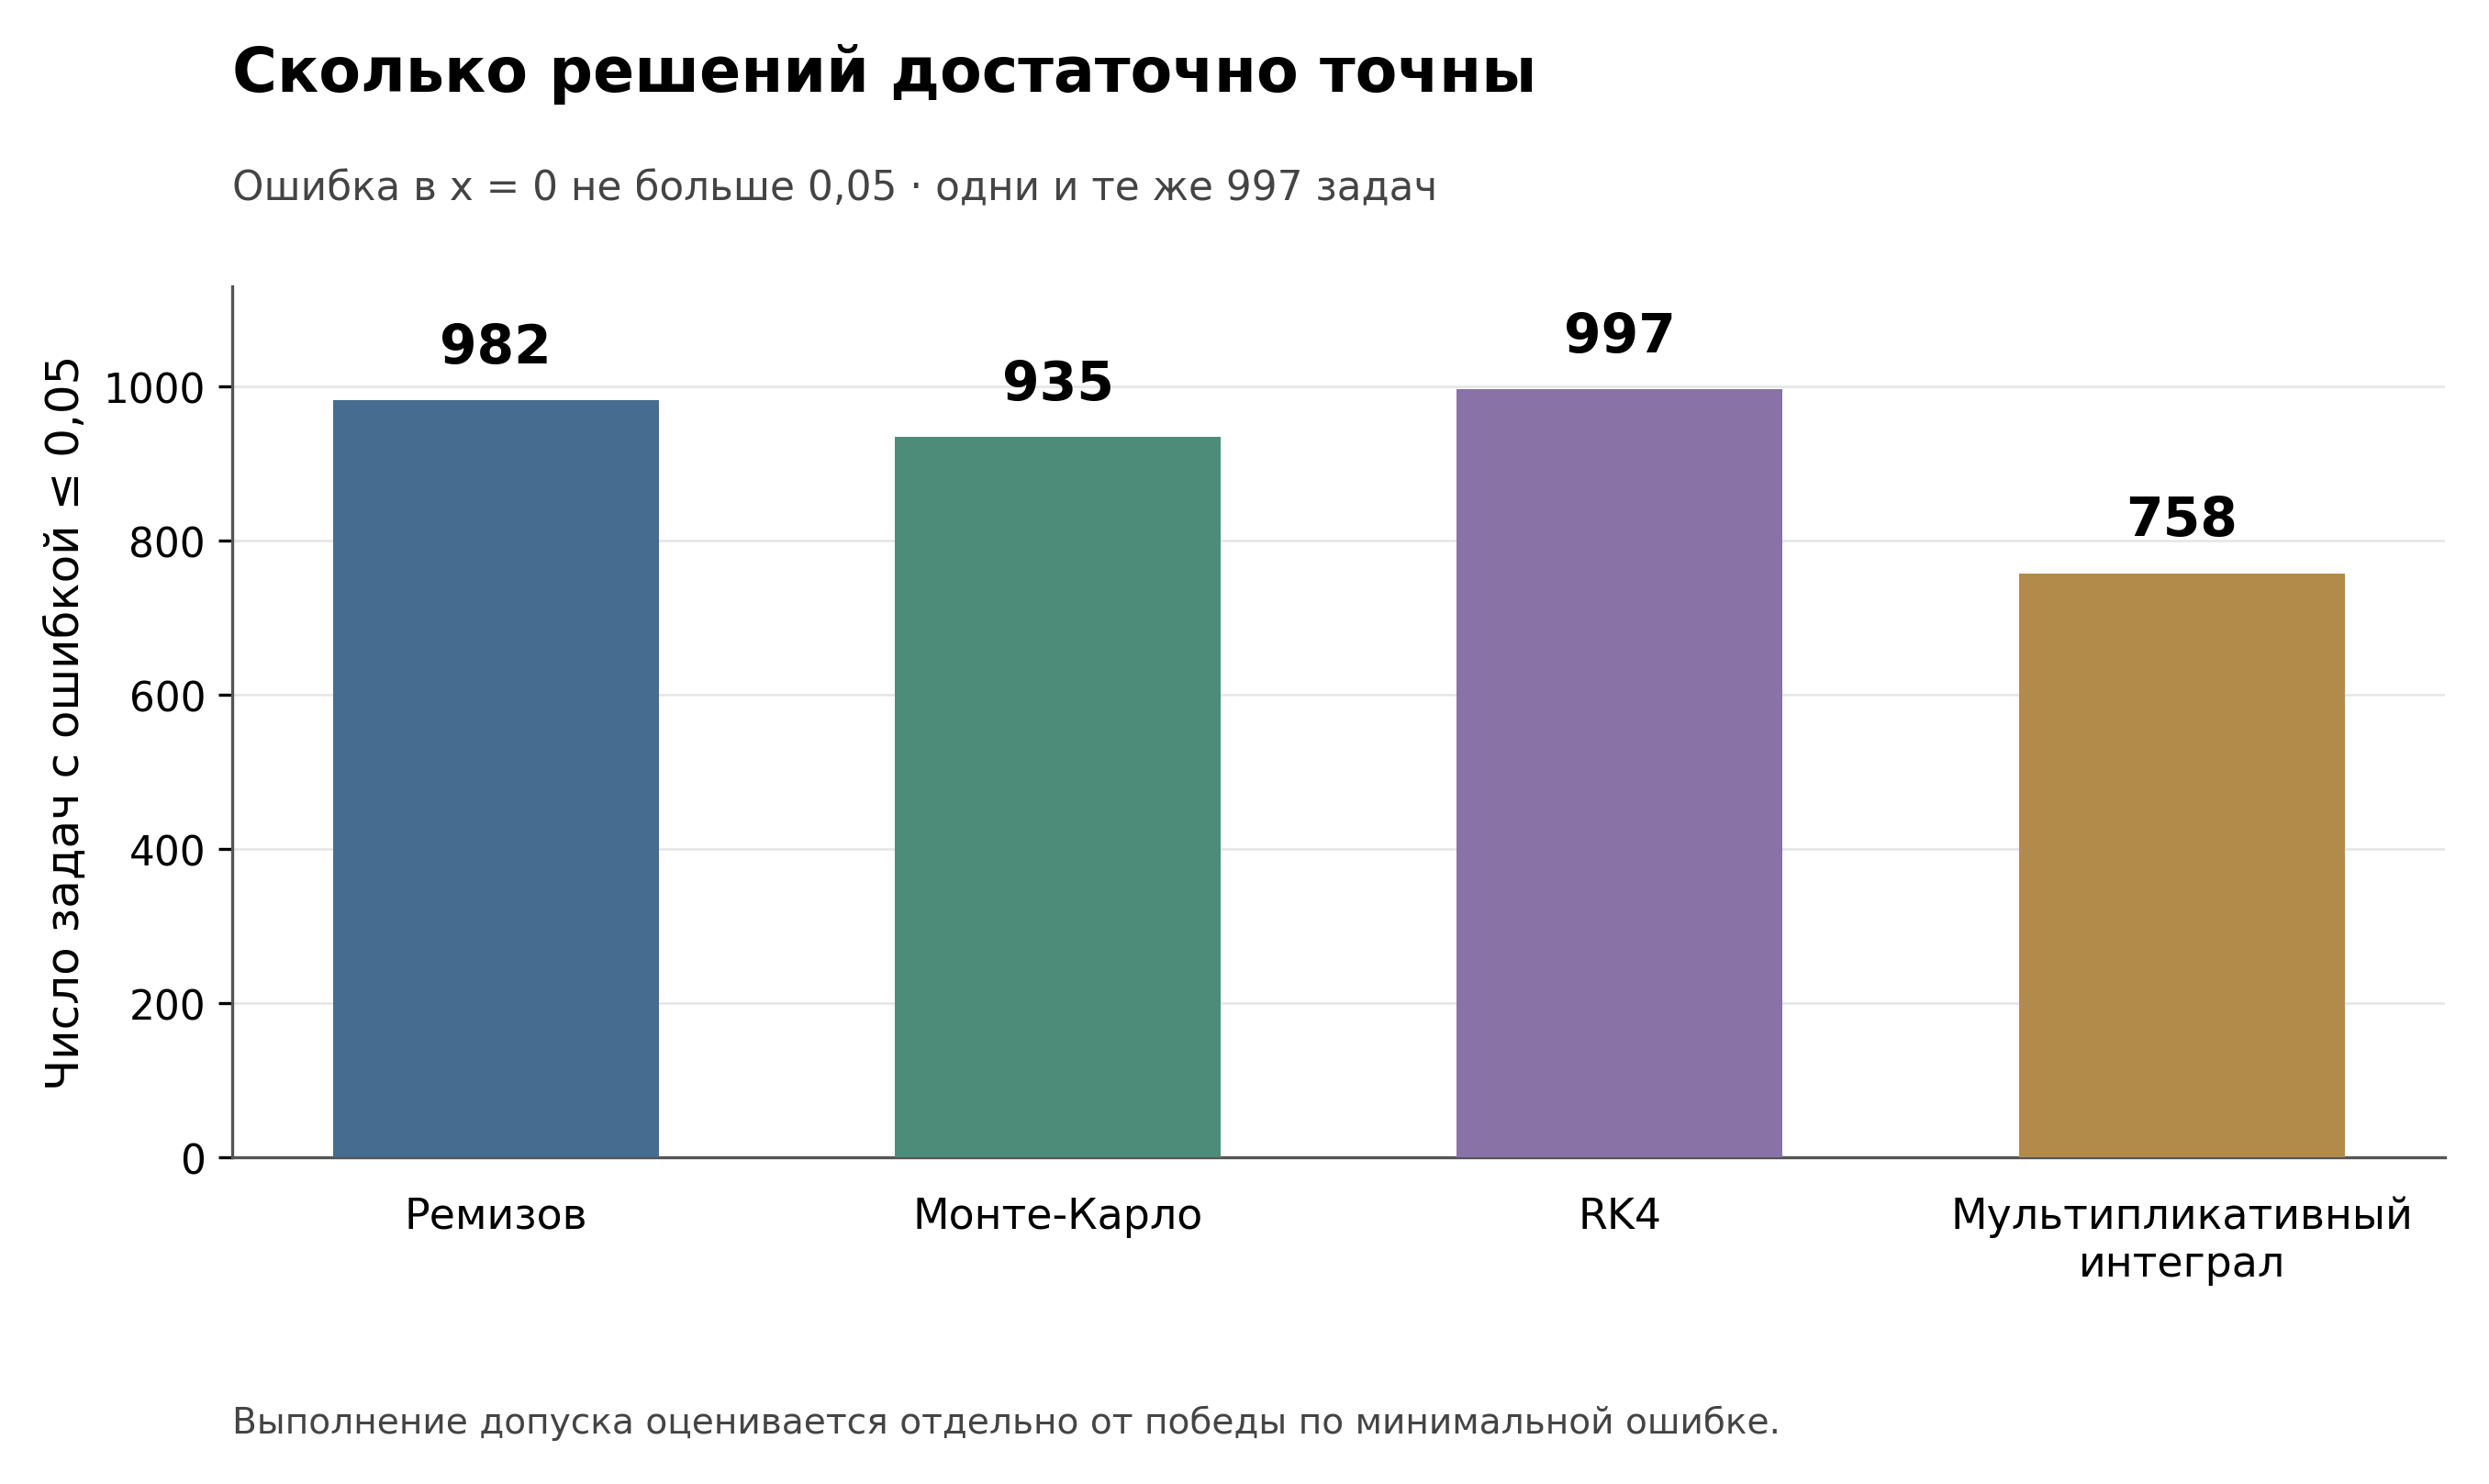
\includegraphics[width=\textwidth]{simple_06_four_methods_success_rate.png}
\caption{Число уравнений, на которых метод достигает точности $0.05$
в точке $x=0$ (997 уравнений). Достижение точности и наименьшая ошибка ---
разные свойства.}
\label{fig:ml-success4}
\end{figure}

Результат этой таблицы и рисунков относится к выбранным настройкам
и к точке $x=0$. Отдельная проверка на 33 узлах приведена
в разделе~\ref{sec:grid33}; она не заменяет точечную метрику.
Расчёт с одним шагом не позволяет оценить
порядок сходимости методов, их устойчивость при других условиях и объём
вычислений, нужный для достижения точности. Время счёта методов в этой
серии не сравнивалось.

Для машинного обучения вывод однозначен: на всех 997 уравнениях лучший
метод --- RK4, и постоянный выбор RK4 уже полностью совпадает с метками.
На таком наборе нельзя содержательно проверить, умеет ли модель различать
области, где лучше разные методы, поэтому модель выбора из четырёх
методов не обучалась.

\clearpage
\subsubsection{Отдельная проверка максимальной ошибки на 33 узлах}\label{sec:grid33}
Чтобы проверить поведение ошибки вне нуля, использованы сохранённые
численные ответы на общей контрольной сетке
\[
G_{33}=\{x_k=-1+k/16:\ k=0,\dots,32\}.
\]
Для неё введена отдельная метрика
\begin{equation}\label{eq:grid33-error}
E_{m,33}=\max_{x_k\in G_{33}}|f_m(x_k)-f(x_k)|.
\end{equation}
Это дискретная максимальная абсолютная ошибка. Она не является
автоматически доказанной нормой $\sup_{x\in[-1,1]}|f_m(x)-f(x)|$:
между узлами могут находиться большие значения ошибки.
Основной точечный эксперимент, ML-метки, обученные модели
и их показатели выше сохраняют определение~\eqref{eq:ml-error}.
Модели по сеточной метрике не обучались.

\paragraph{Сохранённые данные\\}
У метода Ремизова сохранены $f_m(x_k)$ и точные значения во всех
33 узлах для 997 уравнений. У RK4 и мультипликативного интеграла
сохранены полные траектории из 129 узлов; выбирается каждый четвёртый
узел, поэтому дополнительная интерполяция не требуется.
Новые решения ОДУ и MC-траектории для этой проверки не вычислялись.
Источники и правила извлечения указаны в локальных артефактах
проекта~\cite{savedgrid}.

\begin{table}[!htbp]
\centering
\caption{Измеренная ошибка $E_{m,33}$ на общих 997 уравнениях.
Для MC полных данных на этой сетке нет.}
\label{tab:grid33-common}
\resizebox{\textwidth}{!}{%
\begin{tabular}{lccccc}
\toprule
Метод & средняя & медиана & квантиль $0.95$ & максимум & $E_{m,33}\le0.05$\\
\midrule
Ремизова & 39.4119 & 0.002748 & 0.022707 & 19704.502 & 970/997\\
RK4 & $1.208\cdot10^{-6}$ & $2.984\cdot10^{-8}$ & $2.629\cdot10^{-6}$ & $4.578\cdot10^{-4}$ & 997/997\\
Мультипликативный интеграл & 0.273965 & 0.069506 & 0.960674 & 14.383619 & 402/997\\
Монте-Карло & \multicolumn{5}{c}{полная сеточная ошибка не вычислена}\\
\bottomrule
\end{tabular}}
\end{table}

На полном доступном покрытии RK4 достигает $E_{m,33}\le0.05$
на 1000 из 1000 уравнений, мультипликативный интеграл --- на 404
из 1000, Ремизов --- на 970 из 997. Для PI это существенно меньше
точечного результата 760 из 1000. Показатель 402/997
в таблице~\ref{tab:grid33-common} относится к общему поднабору,
а 404/1000 --- ко всем доступным PI-ответам; противоречия нет.


\begin{table}[!htbp]
\centering
\caption{Полное доступное покрытие сохранённой серии. В строке MC
статистики относятся только к нижней оценке $E_{\mathrm{MC},0}$,
а не к неизмеренной $E_{\mathrm{MC},33}$.}
\label{tab:grid33-full}
\resizebox{\textwidth}{!}{%
\begin{tabular}{lrrrrl}
\toprule
Метод и величина & $n$ & Средняя & Медиана & Максимум & Допуск $E_{33}\le0.05$\\
\midrule
Ремизов, $E_{33}$ & 997 & $39.41192$ & $0.002747969$ & $19704.5$ & 970/997\\
RK4, $E_{33}$ & 1000 & $1.204942\cdot10^{-6}$ & $2.984534\cdot10^{-8}$ & $0.000457805$ & 1000/1000\\
PI, $E_{33}$ & 1000 & $0.2735125$ & $0.06942322$ & $14.38362$ & 404/1000\\
MC, $E_0$ & 1000 & $0.01806392$ & $0.009187533$ & $0.5697637$ & \parbox{24mm}{\raggedright $\ge62$ нарушений, 938 неизвестных}\\
\bottomrule
\end{tabular}}
\end{table}

Для MC из нижней оценки следуют 62 нарушения допуска; для остальных
938 задач достижение сеточного допуска неизвестно. Число 938/1000
не является долей сеточно точных MC-решений. Значения полной
$E_{\mathrm{MC},33}$ и её признака точности остаются отсутствующими.
Три отсутствующих R-ответа --- \texttt{F0134/S03}, \texttt{F0136/S01},
\texttt{F0139/S00} --- учитываются отдельно. Их нельзя считать ошибками
нулевой величины или поражениями R; четырёхметодный winner для них
не установлен. Источники полных таблиц и графиков~\cite{savedgrid33release,savedgrid33figures}.

\paragraph{Нижняя оценка для Монте-Карло и победа RK4\\}
В массовой серии MC сохранено среднее четырёх ответов только в нуле.
Рассмотрим дополнение именно этого ответа значениями в остальных
узлах $G_{33}$, без изменения уже полученного значения $f_{\mathrm{MC}}(0)$.
Такое дополнение совместимо с реализованной адресацией случайных
потоков: она зависит от уравнения, координаты и seed, а не от числа
точек. Поскольку $0\in G_{33}$, обязательно выполняется
\begin{equation}\label{eq:mc-grid-lower}
E_{\mathrm{MC},33}\ge
|f_{\mathrm{MC}}(0)-f(0)|=E_{\mathrm{MC}}.
\end{equation}
Для каждого из 997 общих уравнений по неокруглённым сохранённым
значениям проверены строгие неравенства
\begin{equation}\label{eq:rk-grid-dominance}
E_{\mathrm{RK4},33}<
\min\{E_{\mathrm{R},33},\ E_{\mathrm{PI},33},\ E_{\mathrm{MC}}\}.
\end{equation}
Минимальный запас $E_{\mathrm{MC}}-E_{\mathrm{RK4},33}$ составляет
$2.6073122596\cdot10^{-5}$ и наблюдается у
\texttt{AMV1\_F0014\_S01}. Из~\eqref{eq:mc-grid-lower}
и~\eqref{eq:rk-grid-dominance} следует
\[
E_{\mathrm{RK4},33}<E_{\mathrm{MC},33},\qquad
E_{\mathrm{RK4},33}<E_{\mathrm{R},33},\qquad
E_{\mathrm{RK4},33}<E_{\mathrm{PI},33}.
\]
Следовательно, на всех 997 общих уравнениях RK4 остаётся единственным
победителем по сеточному критерию для этих фиксированных реализаций
и сохранённого MC-ответа. Полный MC-расчёт на сетке для данного
вывода не нужен. Но среднюю, медианную, максимальную сеточную ошибку
MC и точное число выполнений сеточного допуска определить нельзя.
Для нового независимого MC-расчёта эти неравенства требуют новой
проверки. Результат не доказывает превосходства RK4 на других задачах,
при другом бюджете или без точных начальных условий.

\paragraph{Пространственная реализация Ремизова\\}
Редкие крупные значения существенно влияют на среднюю ошибку R.
Контролируемое сравнение граничных продолжений и расширение прежней
диагностики до development-выборки рассмотрены отдельно
в разделе~\ref{sec:boundarydev}. Исходные \code{cubic/taper}-ответы
не подменяются экспериментальными в таблицах этого раздела.

Сравнение на одной контрольной сетке не является исследованием
скорости сходимости или сертификацией непрерывной нормы.

\paragraph{Распределения ошибок и выполнение допуска\\}
На рисунке~\ref{fig:grid33-ecdf} сравниваются одинаковые 997 задач.
Логарифмическая ось показывает весь диапазон ошибок без удаления
выбросов. На рисунке~\ref{fig:grid33-hist} приведено полное доступное
покрытие; панель MC относится только к $E_0$ и не является измерением
его сеточного распределения. Все 27 исходных превышений R сохранены
в статистиках и отдельно показаны на рисунке~\ref{fig:grid33-outliers}.
Два крупнейших дают 98.8426\% суммы R-ошибок; это описательное свойство
выборки, а не доказательство причины. На рисунке~\ref{fig:grid33-shares}
знаменатель равен 1000: у R 97\% подтверждённо точных ответов,
2.7\% превышений и 0.3\% пропусков. Среди доступных 997 ответов
точных 97.2919\%. Ошибки внутри семейства зависимы; эти доли не
интерпретируются как независимые популяционные вероятности.

\begin{sidewaysfigure}[p]
\centering
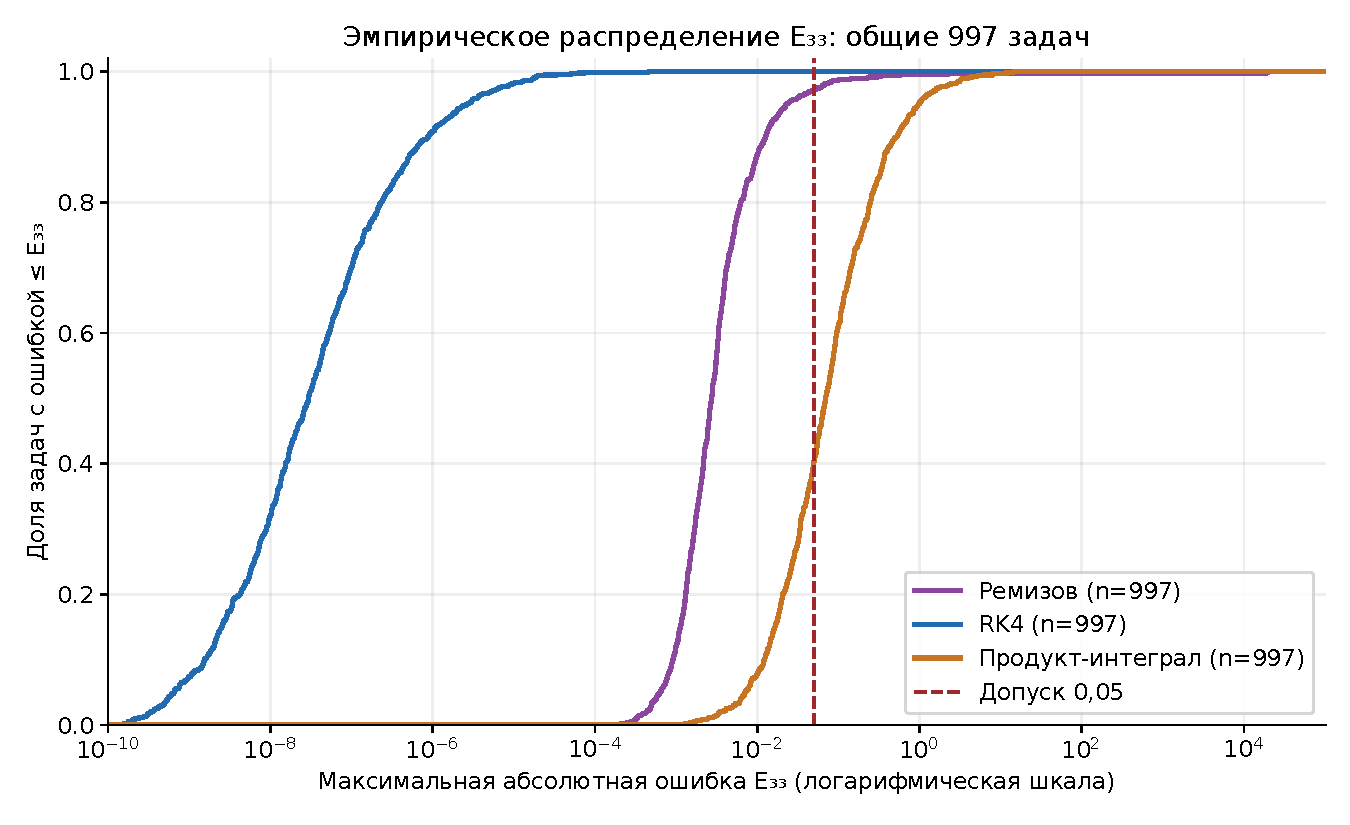
\includegraphics[width=0.94\textheight,height=0.64\paperwidth,keepaspectratio]{grid33_01_ecdf_common997.pdf}
\caption{Накопленное распределение измеренных $E_{33}$ на общих 997 задачах. Логарифмическая ось ошибок; пунктиром показан допуск $0.05$. Полная MC~$E_{33}$ отсутствует.}
\label{fig:grid33-ecdf}
\end{sidewaysfigure}

\begin{sidewaysfigure}[p]
\centering
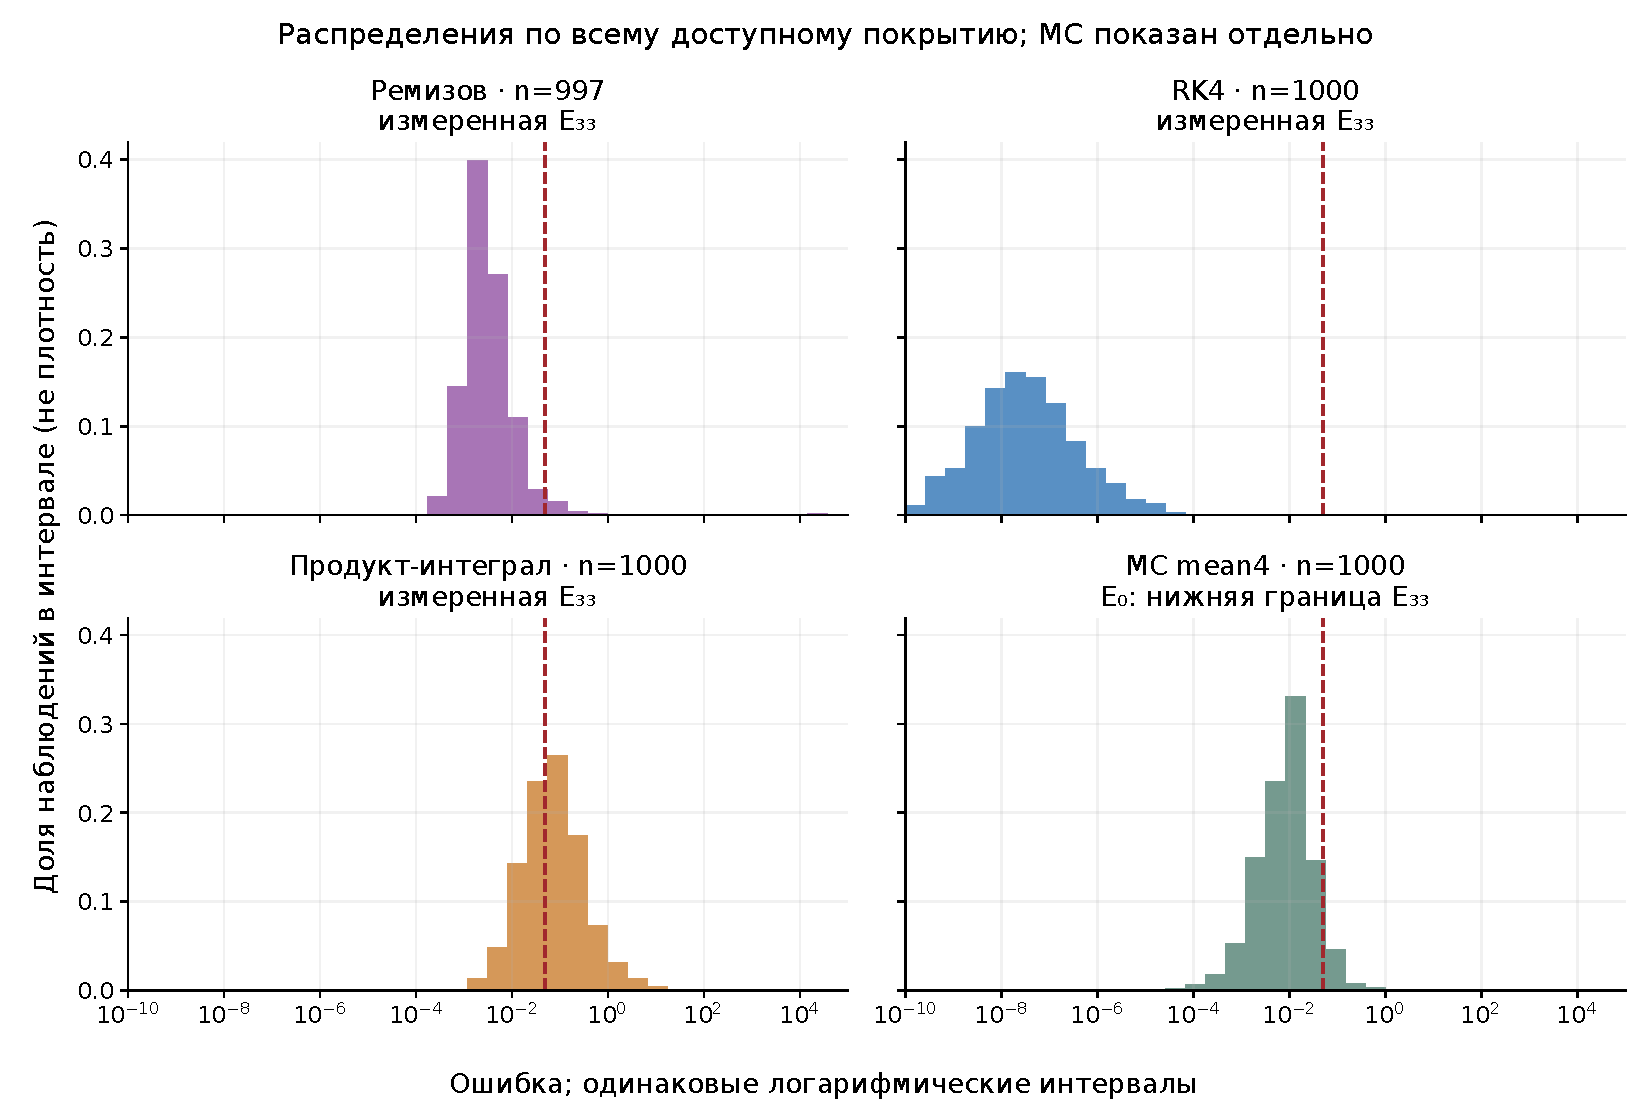
\includegraphics[width=0.94\textheight,height=0.64\paperwidth,keepaspectratio]{grid33_02_histograms_available.pdf}
\caption{Распределения по всему доступному покрытию; одинаковые логарифмические интервалы. Ордината --- доля наблюдений в интервале, не плотность. Отдельная MC-панель показывает лишь нижнюю оценку $E_0$. Пунктир --- $0.05$.}
\label{fig:grid33-hist}
\end{sidewaysfigure}

\begin{sidewaysfigure}[p]
\centering
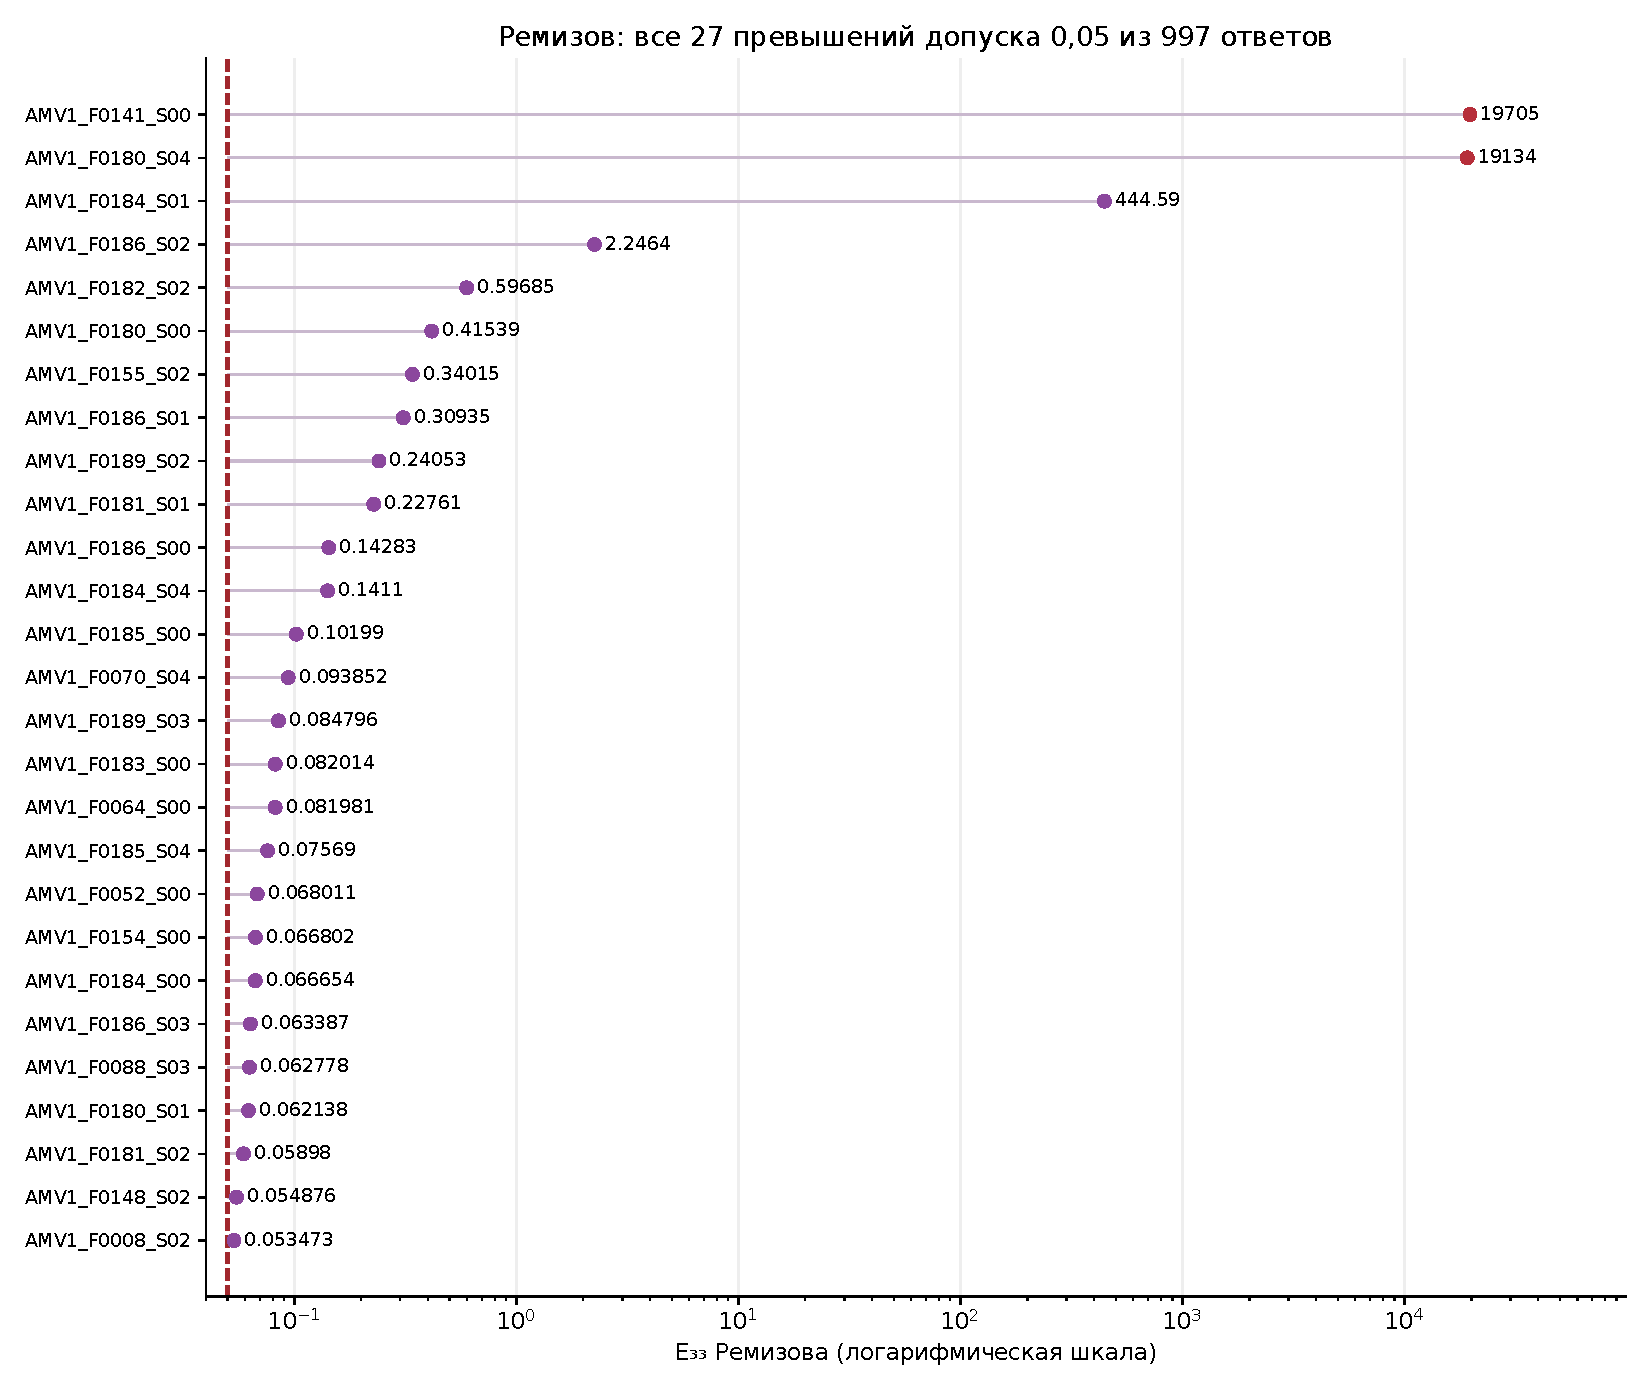
\includegraphics[width=0.94\textheight,height=0.64\paperwidth,keepaspectratio]{grid33_03_remizov_exceedances.pdf}
\caption{Все 27 исходных ответов R с $E_{33}>0.05$. Два крупнейших выделены цветом. Выбросы не удалены из исходной статистики; термин используется описательно.}
\label{fig:grid33-outliers}
\end{sidewaysfigure}

\begin{sidewaysfigure}[p]
\centering
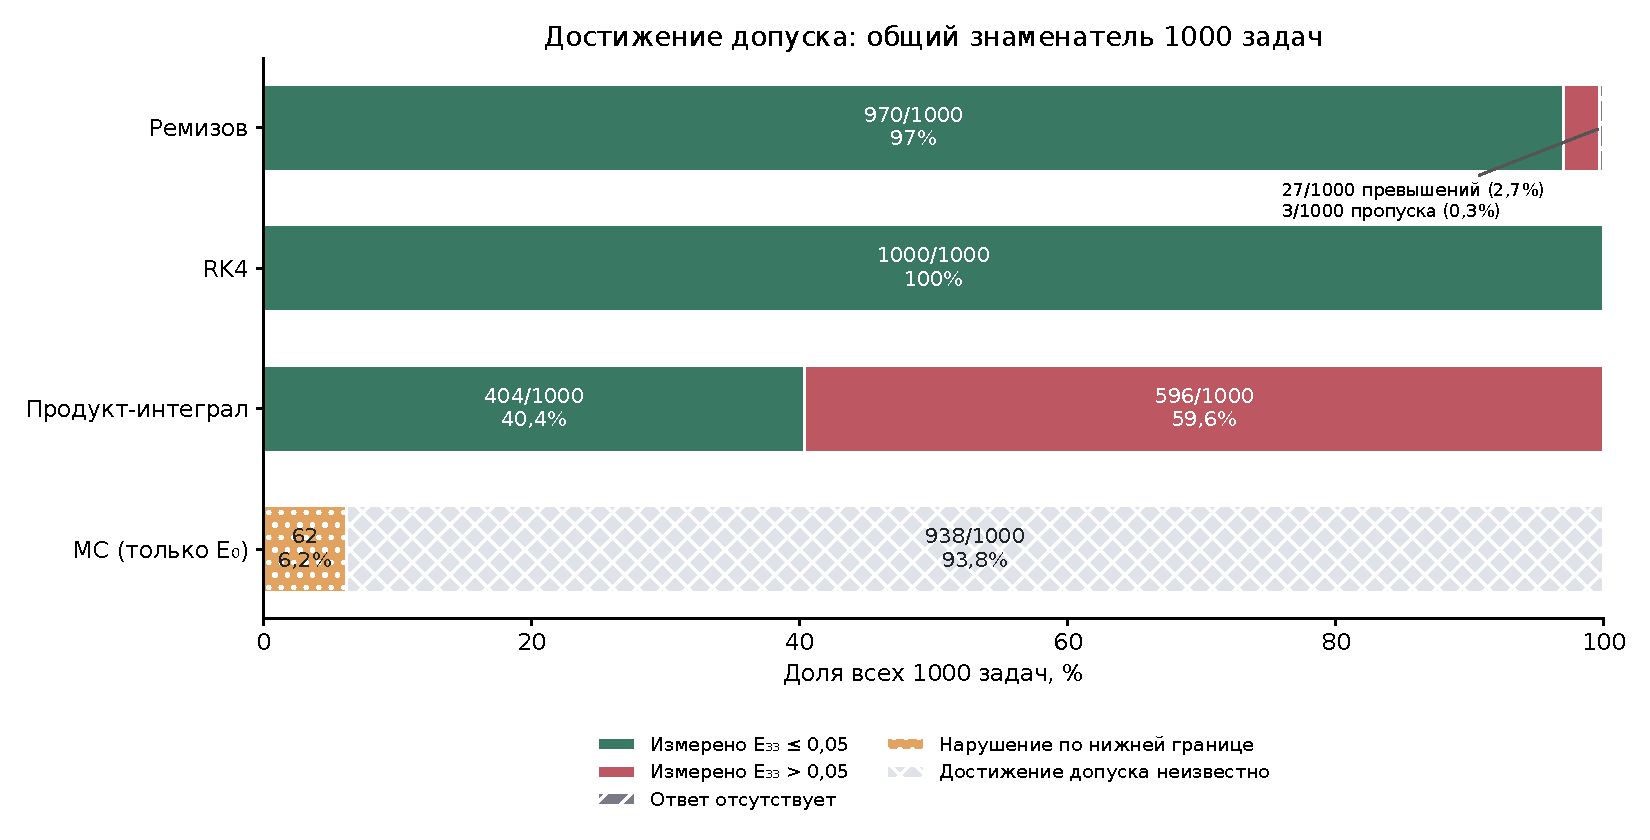
\includegraphics[width=0.94\textheight,height=0.64\paperwidth,keepaspectratio]{grid33_04_threshold_shares.pdf}
\caption{Доли от всех 1000 задач. Пропуски R отделены от измеренных превышений. Для MC 62 нарушения следуют только из нижней оценки, в 938 случаях выполнение допуска неизвестно; это не 938 сеточно точных ответов.}
\label{fig:grid33-shares}
\end{sidewaysfigure}

\clearpage
\subsubsection{Пилот минимизации стоимости при заданной сеточной точности}
\label{sec:costpilot}

Преимущество по ошибке при фиксированных параметрах ещё не определяет,
возникает ли полезная задача выбора метода по времени. В отдельном
ограниченном пилоте~\cite{savedcost60} сравнивались только RK4 и
мультипликативный интеграл (PI) при $N=32,64,128,256$ и допуске
$E_{m,33}\le0.01$. Этот пилот не включал обучение моделей.

\paragraph{Выборка и протокол измерения\\}
Детерминированно отобраны 60 задач исходной обучающей части из 60 разных
семейств и топологий: по три задачи из каждой из 20 ячеек
«сложность~$\times$~режим». Представитель семейства задавался хешем
идентификатора с фиксированным seed, разнообразие коэффициентов
обеспечивалось maximin-отбором по нормированным входным характеристикам.
Ошибки, времена, прогнозы моделей и значения точного решения при выборе
не использовались. Исторические тестовые семейства и топологии были
исключены. Это целевая разнообразная выборка, а не случайная выборка,
по которой можно оценить частоты в генеральной совокупности.

Оба неизменённых решателя получали одни и те же коэффициенты задачи Коши
на $[-1,1]$ и точные начальные условия $f(-1),f'(-1)$.
Для каждого $N$ контрольные узлы $G_{33}$ точно совпадают с узлами
траектории с индексами $kN/32$, $k=0,\ldots,32$; интерполяция не
применялась. Порог включает равенство. Во всех сравнениях используется
именно дискретная ошибка~\eqref{eq:grid33-error}.

На одном компьютере в одном процессе для каждой из 480 пар
«задача~$\times$~конфигурация» выполнены один прогрев и пять измеряемых
повторов: 480 прогревочных и 2400 измеряемых вызовов. Порядок вызовов
детерминированно перемешивался в каждом раунде. Основной показатель
$t_i(m,N)$ --- медиана пяти времён публичного solver-вызова, включающего
вычисление коэффициентов, численные шаги и создание результата.
Загрузка, подготовка точных значений, вычисление ошибки и запись на диск
в этот показатель не включены. Сборщик мусора отключался на измеряемой
фазе, его вызовы выполнялись вне таймера.

Отдельно зарегистрированы импорт (0.208656~с), загрузка и валидация
датасета (2.885793~с), подготовка выбранных входов и точных значений
с вводом-выводом (0.913157~с). Окружение: macOS~26.6.2, arm64,
Python~3.10.11, NumPy~2.2.6, SciPy~1.15.3. Переменные ограничения
внутренних потоков были установлены в~1 до импорта библиотек, однако
\code{threadpoolctl} вернул пустой список. Тепловые и performance-сведения
через \code{pmset} получить не удалось. Поэтому фактическое число
внутренних потоков и отсутствие теплового ограничения частоты независимо
не подтверждены; времена характеризуют эту машину и данный протокол.

\begin{table}[!htbp]
\centering
\caption{Пилот стоимости: точность восьми конфигураций на 60 задачах.
Время --- среднее по задачам от медианы пяти повторов solver;
оно не включает подготовку данных.}
\label{tab:costpilot-configurations}
\small
\begin{tabular}{lrcrc}
\toprule
Метод & $N$ & $E_{m,33}\le0.01$ & Время, мс & $\max E_{m,33}$\\
\midrule
RK4 & 32  & 59/60 & 60.077893  & $1.366209\cdot10^{-2}$\\
RK4 & 64  & 60/60 & 119.962860 & $2.747976\cdot10^{-4}$\\
RK4 & 128 & 60/60 & 239.217672 & $1.699437\cdot10^{-5}$\\
RK4 & 256 & 60/60 & 478.999962 & $1.058317\cdot10^{-6}$\\
PI  & 32  & 0/60  & 15.686458  & 15.916198\\
PI  & 64  & 0/60  & 31.300706  & 8.039300\\
PI  & 128 & 4/60  & 62.703981  & 4.037363\\
PI  & 256 & 7/60  & 125.386115 & 2.022754\\
\bottomrule
\end{tabular}
\end{table}

\paragraph{Oracle и постоянные правила\\}
Oracle для каждой задачи выбирает конфигурацию с минимальной измеренной
медианой среди удовлетворяющих допуску. Лучшая постоянная конфигурация
должна удовлетворять допуску на всех 60 задачах и минимизировать сумму
медиан. Для отделения выбора метода от выбора шага дополнительно
рассмотрен oracle, которому доступны только конфигурации RK4.
Все эти правила определены по уже известным точным ошибкам. Они дают
ретроспективное сравнение и не являются готовыми адаптивными алгоритмами:
стоимость пробных решений и поиска допустимого $N$ в них не учтена.

\begin{table}[!htbp]
\centering
\caption{Стоимость выбора при одинаковом выполнении допуска на 60/60
задачах. Сумма складывается из медиан отдельных solver-вызовов.}
\label{tab:costpilot-selection}
\small
\begin{tabular}{p{0.48\textwidth}rr}
\toprule
Правило & Среднее, мс & Сумма, с\\
\midrule
Лучшая постоянная конфигурация: RK4, $N=64$
 & 119.962860 & 7.197772\\
Oracle по RK4 и PI
 & 62.038960 & 3.722338\\
Oracle только по RK4
 & 62.038960 & 3.722338\\
\bottomrule
\end{tabular}
\end{table}

Во всех 60 случаях oracle выбрал RK4 (100\%); PI не выбран ни разу
(0\%). Для 59 задач достаточно $N=32$, для одной --- $N=64$.
Исключение --- \code{AMV1\_F0186\_S00}: при $N=32$
$E_{\mathrm{RK4},33}=0.0136620881782$, при $N=64$ ---
$0.000210115440205$. Задач, для которых ни одна из восьми конфигураций
не достигла допуска, нет; неизвестных исходов из-за отказов также нет.
PI имеет хотя бы одну допустимую конфигурацию на семи задачах,
но на каждой уступает по медиане подходящей конфигурации RK4.

Среднее относительное сокращение времени oracle относительно постоянного
RK4 при $N=64$ равно $49.1967\%$, а сокращение суммы времён ---
$48.2849\%$. Это разные показатели:
\[
\frac1{60}\sum_{i=1}^{60}
\left(1-\frac{t_i^{\mathrm{oracle}}}{t_i^{\mathrm{const}}}\right),
\qquad
1-\frac{\sum_i t_i^{\mathrm{oracle}}}{\sum_i t_i^{\mathrm{const}}}.
\]
Средняя абсолютная экономия составляет 57.923901~мс на задачу.
Весь выигрыш достигается выбором числа шагов внутри RK4:
добавление PI к RK4-only oracle даёт ровно $0\%$.
Правило минимального допустимого $N$ для RK4 совпало с этим oracle
на всех 60 задачах.

До запуска были зафиксированы критерии GO: не менее 12 из 60 побед
каждого метода и не менее 12 устойчивых побед каждого; не менее 10\%
выигрыша по обоим приведённым показателям относительно лучшей константы
и RK4-only oracle; полное покрытие допуска и не менее 90\% стабильных
профилей. Устойчивая победа требует запаса по медиане не менее 10\%,
неперекрытия интервалов наблюдаемых времён
$\max t_{\rm fast}<\min t_{\rm slow}$ и
$\mathrm{MAD}/\mathrm{median}\le0.20$ у обеих конфигураций.
Это операционные критерии практической полезности, а не статистический
тест значимости. Все 480 профилей удовлетворили ограничению по MAD;
56 методных побед RK4 устойчивы, в четырёх практический запас не
подтверждён. Эти четыре случая не являются победами PI.

\textbf{Результат пилота --- NO-GO для дальнейшего ML выбора между RK4
и PI в данной постановке.} Не получены неоднородность победителей,
устойчивые победы обоих методов и добавочная экономия относительно
выбора $N$ только внутри RK4. Полезность предсказания редкой необходимости
увеличить $N$ отдельно не проверена. Данные пилота не доказывают
обучаемость селектора, переносимость времён, порядок сходимости или
универсальное превосходство RK4. Сохранённая независимая проверка
сверила все ячейки CSV, 2880 ошибок по вложенным узлам и 2400 измерений
времени без новых solver-вызовов~\cite{savedcost60}.

\clearpage
\subsubsection{Граничное продолжение Ремизова на development-выборке}
\label{sec:boundarydev}

Предыдущая диагностика двух экстремальных ответов~\cite{savedboundary}
показала сильное уменьшение ошибки при замене внешнего продолжения
\code{cubic/taper} на \code{cubic/zero}. Для проверки границ этого
наблюдения выполнено одно ограниченное исследование~\cite{savedboundarydev}.
Оно проверяет конкретную реализацию на конечном пространственном окне,
сохраняя математическую формулу метода и исходный производственный
профиль \code{cubic/taper}.

\paragraph{Выборка и контролируемое изменение\\}
Включены все 22 доступные development-задачи с исходной
$E_{\mathrm{R},33}>0.05$ и 30 заранее выбранных контролей с
$E_{\mathrm{R},33}\le0.05$. Проблемная группа охватывает 14 семейств;
контроли взяты из 30 других попарно различных семейств с
детерминированной стратификацией по 20 ячейкам сложности и режима.
Исторические тестовые семейства и топологии исключены, результаты
\code{zero} при отборе не использовались. Три отсутствующих исходных
development-ответа Ремизова не имеют измеренной $E_{\mathrm{R},33}$,
поэтому не входят в эти 52 задачи и не заменяются условной ошибкой.
Прежняя задача \code{F0180/S04} принадлежит Test и в новую оценку не
включалась; в исторической диагностике её ошибка уменьшилась с
19134.405 до 0.0704519 и осталась выше допуска 0.05~\cite{savedboundary}.

Для всех 52 задач повторно использованы исходные ответы \code{taper};
два полностью совместимых ответа \code{zero} также взяты из сохранённых
результатов. Выполнено ровно 50 новых вызовов \code{zero} и ни одного
нового вызова \code{taper}. В сравнении изменён только параметр внешнего
продолжения. Сохранены $n=128$, 513 временных узлов с квадратичным
размещением, $\Delta x=0.0125$, дополнение окна на 12 с каждой стороны
интервала $[-1,1]$, то есть окно $[-13,13]$ из 2081 узла,
и $\code{tail\_eps}=10^{-8}$. Эффективное $T$ совпадает для каждого
идентификатора. Совпадение коэффициентов, точного решения,
пространственных и временных сеток, квадратурных весов и $G_{33}$
проверено по исходным значениям и контрольным суммам. Другие продолжения,
MC и ML в этой серии не исследовались.

Порог точности равен $0.05$. Катастрофическим выбросом в протоколе
условно названо $E_{\mathrm{R},33}>1$; это определение исхода,
а не утверждение о математической неприменимости метода.
Для разности $\Delta E=E^{\mathrm{zero}}-E^{\mathrm{taper}}$
заранее задан допуск численного сравнения
\[
\delta_i=10^{-10}\max\{1,E_i^{\mathrm{taper}}\}.
\]
Уменьшение означает $\Delta E<-\delta_i$, совпадение ---
$|\Delta E|\le\delta_i$, регрессия по этому критерию ---
$\Delta E>\delta_i$. Этот допуск не является ни границей полной ошибки,
ни порогом практической существенности.

\begin{table}[!htbp]
\centering
\caption{Результат замены \code{taper} на \code{zero}.
Уменьшения, совпадения и регрессии определены с допуском $\delta_i$.
Столбцы с парой значений относятся к исходному и новому продолжению.}
\label{tab:boundarydev-groups}
\resizebox{\textwidth}{!}{%
\begin{tabular}{lrrrrrr}
\toprule
Группа & $n$ & \parbox{23mm}{\centering $E_{33}\le0.05$, до/после} & Снижений & Равенств
 & Регрессий & \parbox{20mm}{\centering $E_{33}>1$, до/после}\\
\midrule
Проблемные & 22 & 0/1 & 9 & 10 & 3 & 3/0\\
Контроли & 30 & 30/30 & 2 & 28 & 0 & 0/0\\
Все & 52 & 30/31 & 11 & 38 & 3 & 3/0\\
\bottomrule
\end{tabular}}
\end{table}

\paragraph{Устранённые выбросы и оставшиеся ошибки\\}
Все три исходных выброса выше единицы опустились ниже единицы
(таблица~\ref{tab:boundarydev-extremes}). Это подтверждает влияние
граничного продолжения на данные выбросы при фиксированных остальных
параметрах. Однако только одна из 22 проблемных задач перешла ниже 0.05;
21 задача осталась вне допуска. Максимум по 52 задачам уменьшился
с 19704.5019109 до 0.596851548154. У всех 30 контролей допуск сохранён;
новых выбросов выше единицы и неуспешных ответов \code{zero} нет.

\begin{table}[!htbp]
\centering
\caption{Три исходных катастрофических выброса development-выборки.
Приведены итоговые ошибки на $G_{33}$, а не промежуточные состояния.}
\label{tab:boundarydev-extremes}
\small
\begin{tabular}{lrrc}
\toprule
Задача & $E_{33}$, \code{taper} & $E_{33}$, \code{zero}
 & Допуск после\\
\midrule
\code{F0141/S00} & 19704.5019109 & 0.0187192785409 & да\\
\code{F0184/S01} & 444.589254639 & 0.0535680732159 & нет\\
\code{F0186/S02} & 2.24644415774 & 0.254377736872 & нет\\
\bottomrule
\end{tabular}
\end{table}

Положительная неокруглённая разность наблюдается у 19 задач, включая
увеличения меньше $\delta_i$. Только три разности превышают заранее
заданный допуск сравнения (таблица~\ref{tab:boundarydev-regressions}).
Все три задачи уже находились выше 0.05; новых потерь допуска нет.
Приращения порядка $10^{-9}$ не свидетельствуют об установленном
практически значимом ухудшении.

\begin{table}[!htbp]
\centering
\caption{Все три регрессии, превышающие $\delta_i$.
Относительное увеличение приведено как доля, а не процент.}
\label{tab:boundarydev-regressions}
\small
\begin{tabular}{lcc}
\toprule
Задача & $\Delta E_{33}$ & $\Delta E_{33}/E_{33}^{\mathrm{taper}}$\\
\midrule
\code{F0186/S01} & $6.098373472873675\cdot10^{-10}$ & $1.9713427\cdot10^{-9}$\\
\code{F0189/S02} & $1.312633113315087\cdot10^{-9}$ & $5.4572689\cdot10^{-9}$\\
\code{F0189/S03} & $6.146191888767305\cdot10^{-10}$ & $7.2482444\cdot10^{-9}$\\
\bottomrule
\end{tabular}
\end{table}

\paragraph{Пространственная аппроксимация и теоретические ограничения\\}
В \code{zero} неизменённый внутренний кубический сплайн используется
внутри окна, а запросам строго за окном присваивается ноль.
Граничный узел при этом сохраняет своё вычисленное значение. Если оно
ненулевое, продолжение разрывно и не принадлежит пространствам
непрерывных ограниченных функций $C_b$ или $UC_b$, когда они требуются
в теоретическом обосновании. Это не отдельный решатель корректно
поставленной краевой задачи с условием Дирихле: граничные узловые
значения принудительно не обнуляются. Даже при нулевых концах гладкость
продолжения не гарантирована. Например, сплайн через узлы
$x=(0,1,2,3)$ со значениями $(0,1,1,0)$ равен
$p(x)=3x/2-x^2/2$; его производные на концах равны $3/2$ и $-3/2$,
а производная внешнего нуля равна нулю.

Независимые сохранённые проверки~\cite{savedboundarydev} показывают
также отсутствие гарантии положительности и контрактности
\emph{дискретной кубической реконструкции в узловой максимальной норме}.
При $x=(0,1,2,3)$, $a=1/4$, $b=4$, $c=0$, $\tau=1/16$
и \code{boundary=zero} неизменённая реализация одного применения
$\Sop(\tau)$ даёт в узле $x=1$ значение $67/64>1$ для данных
$u=(0,1,1,0)$ с узловой нормой~1. Для неотрицательных узловых данных
$u=(1,0,0,0)$ результат в том же узле равен $-1/64$.
Это контрпримеры для операции «кубическая реконструкция плюс сдвиги»
на векторе узловых значений, а не для точного оператора $\Sop$ на
непрерывных функциях: сама реконструкция может превышать диапазон
узловых данных. Формальные веса $1/4,1/4,1/2$ не дают автоматически
оценку нормы полученного сеточного оператора.

Исходная правая часть имеет носитель внутри окна, но повторные сдвиги
распространяют промежуточные состояния. Поэтому начальная компактность
носителя не исключает последующего влияния границ. Сохранённая величина
\code{boundary\_state\_max\_abs} характеризует эти промежуточные
состояния и не равна итоговой $E_{\mathrm{R},33}$.
Формула $\Sop$, коэффициенты и их глобальные сертификаты сохранены;
пространственная устойчивость, погрешность усечения окна и выполнение
всех предпосылок глобальной теоремы для этой конечномерной реализации
не сертифицированы. Уточнения $\Delta x$, окна, $T$, квадратуры и $n$
в данном сравнении не выполнялись, поэтому причинные доли оставшихся
источников полной ошибки не установлены.

До получения новых ответов GO требовал пригодности всех результатов,
отсутствия регрессий по $\delta_i$, потерь допуска и новых выбросов выше
единицы, устранения всех прежних выбросов выше единицы, увеличения числа
точных ответов и хотя бы одного уменьшения сверх $\delta_i$.
Не выполнено только условие отсутствия регрессий.
\textbf{Формальный итог --- NO-GO для принятия \code{cubic/zero}
как нового экспериментального профиля без регрессий по этому протоколу.}
Критерий не ослаблялся после наблюдений. Этот итог чувствителен к
строгости численного порога и не означает доказанной практической
вредности \code{zero}; сильное уменьшение трёх выбросов остаётся
подтверждённым результатом. Вместе с тем \code{zero} не устраняет
все крупные ошибки и не обеспечивает автоматически теоретическую
корректность пространственной аппроксимации. Исходный производственный
профиль и основные массовые таблицы не заменялись.
Независимая проверка сверила 1664 ячейки таблицы, все 52 ошибки каждого
профиля, два повторно использованных ответа и журнал
50 новых вызовов; проверка не решала ОДУ повторно~\cite{savedboundarydev}.


\subsubsection{Выбор из трёх методов}\label{sec:ml3-res}
Сохранённые метрики и их проверка приведены в источнике~\cite{savedthreeML}.
Если не рассматривать RK4, лучшими оказываются разные методы:
на 997 уравнениях метод Ремизова точнее двух других на 826, Монте-Карло ---
на 106, мультипликативный интеграл --- на 65 (рис.~\ref{fig:ml3-wins},
таблица~\ref{tab:ml3-split}). Результаты модели на тестовой выборке
приведены в таблице~\ref{tab:ml3-test}.

\begin{figure}[!htbp]
\centering
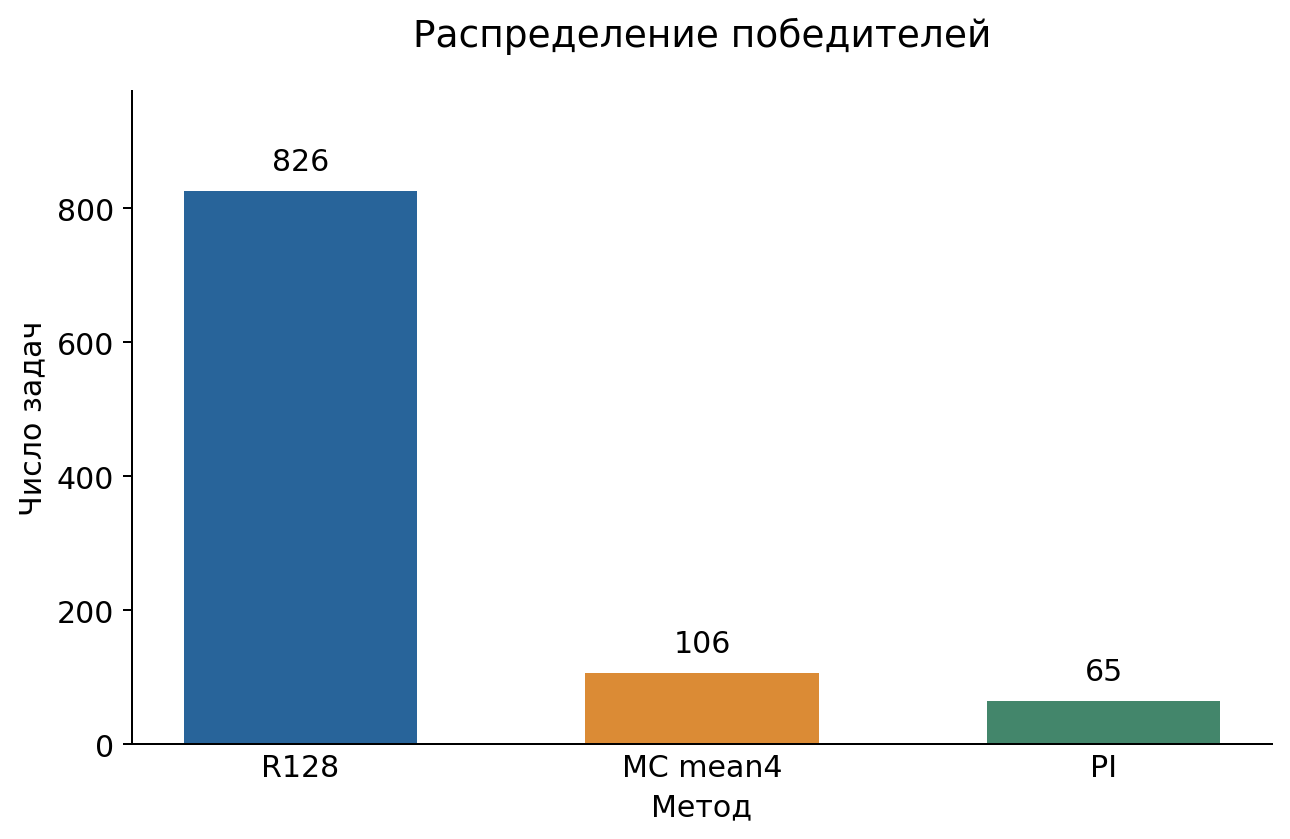
\includegraphics[width=0.8\textwidth]{01_winners.png}
\caption{Число уравнений, на которых каждый из трёх методов даёт
наименьшую ошибку в точке $x=0$ (997 уравнений). R128 --- метод Ремизова
при $n=128$, MC mean4 --- среднее четырёх расчётов Монте-Карло,
PI --- метод мультипликативного интеграла.}
\label{fig:ml3-wins}
\end{figure}

\begin{table}[!htbp]
\centering
\caption{Модель выбора из трёх методов и постоянный выбор одного метода
на тестовой выборке (150 уравнений).}
\label{tab:ml3-test}
\resizebox{\textwidth}{!}{%
\begin{tabular}{lcccc}
\toprule
Правило выбора & Accuracy & macro-F1 & $E\le0.05$ & средняя $E$\\
\midrule
модель & 88.67\% & 0.314 & 147/150 & 1.65885\\
всегда метод Ремизова & 90.67\% & 0.317 & 147/150 & 1.65896\\
всегда Монте-Карло & 4.67\% & 0.030 & 141/150 & 0.01728\\
всегда мультипликативный интеграл & 4.67\% & 0.030 & 110/150 & 0.05416\\
\bottomrule
\end{tabular}}
\end{table}

Модель верно определила лучший метод на 133 из 150 тестовых уравнений
(88.67\%), а выбранный ею метод достиг точности $0.05$ на 147 уравнениях
(98\%). Постоянный выбор метода Ремизова верен на 136 уравнениях
(90.67\%) и тоже достигает точности на 147. Модель выбрала метод
Ремизова 146 раз, Монте-Карло --- 4 раза, мультипликативный интеграл
не выбрала ни разу.

Матрица ошибок модели (строки --- метод, который на самом деле точнее,
столбцы --- выбор модели; порядок: метод Ремизова, Монте-Карло,
мультипликативный интеграл) имеет вид
\[
\begin{pmatrix}
133&3&0\\
7&0&0\\
6&1&0
\end{pmatrix}
\]
(рис.~\ref{fig:ml3-conf}). Все четыре выбора Монте-Карло ошибочны:
в трёх случаях точнее был метод Ремизова, в одном --- мультипликативный
интеграл. Ни одно из 7 уравнений, где точнее Монте-Карло, и ни одно
из 7, где точнее мультипликативный интеграл, модель не нашла. Поэтому
для этих двух методов $F_1=0$, и macro-F1 у модели и у постоянного
выбора метода Ремизова почти одинаков и мал (рис.~\ref{fig:ml3-acc}).

\begin{figure}[!htbp]
\centering
\begin{minipage}[t]{0.49\textwidth}
\centering
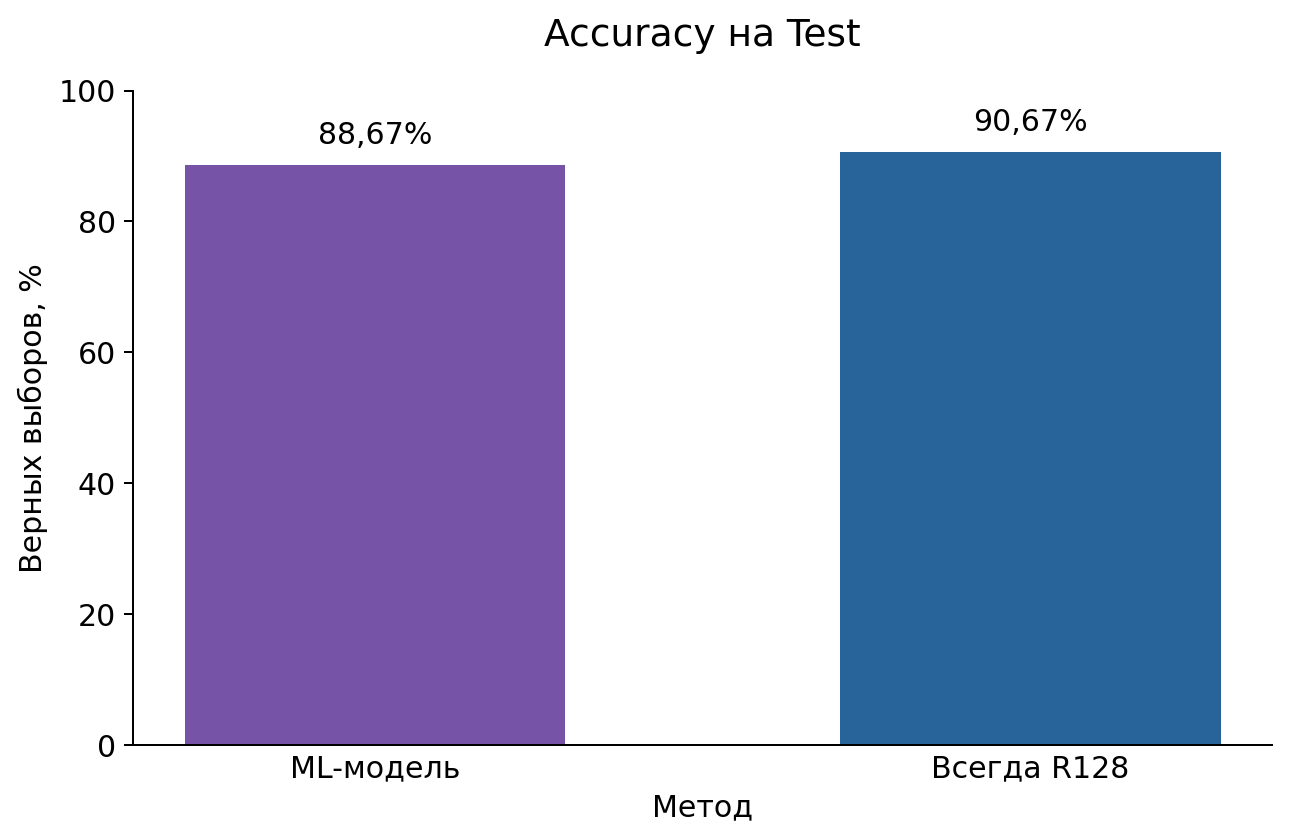
\includegraphics[width=\linewidth]{02_accuracy.png}
\end{minipage}\hfill
\begin{minipage}[t]{0.49\textwidth}
\centering
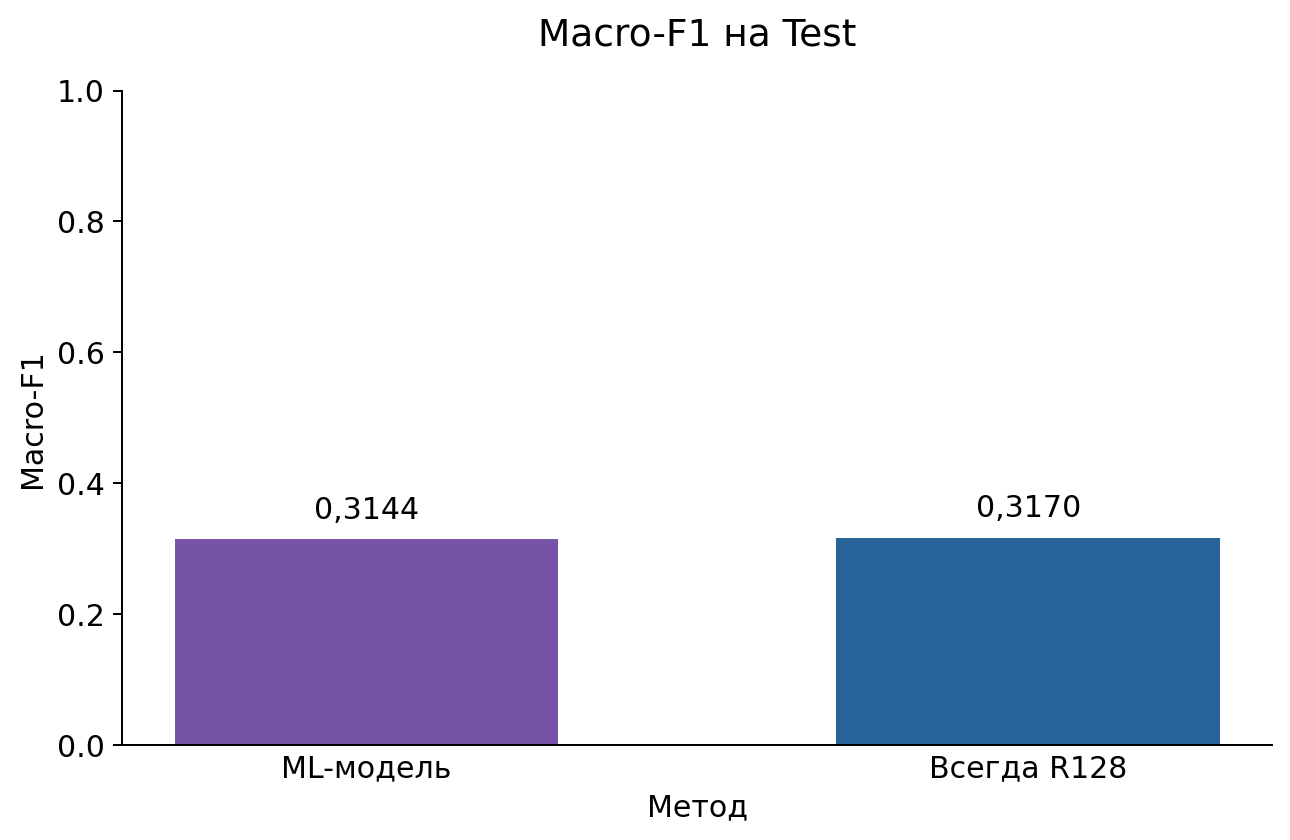
\includegraphics[width=\linewidth]{03_macro_f1.png}
\end{minipage}
\caption{Доля верных выборов (слева) и macro-F1 (справа) на тестовой
выборке для модели и для постоянного выбора метода Ремизова
(на рисунке --- <<Всегда R128>>).}
\label{fig:ml3-acc}
\end{figure}

\begin{figure}[!htbp]
\centering
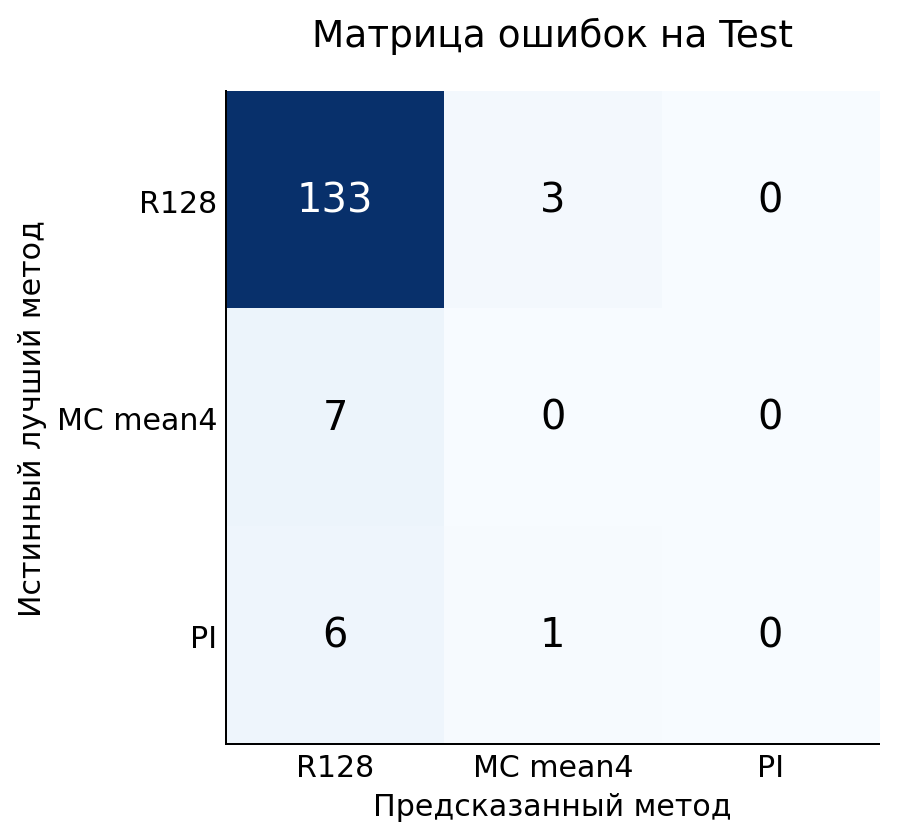
\includegraphics[width=0.6\textwidth]{05_confusion_matrix.png}
\caption{Матрица ошибок модели выбора из трёх методов на тестовой
выборке: по строкам --- метод, который на самом деле точнее,
по столбцам --- метод, выбранный моделью. R128 --- метод Ремизова,
MC mean4 --- Монте-Карло, PI --- мультипликативный интеграл.}
\label{fig:ml3-conf}
\end{figure}

Средние ошибки модели и постоянного выбора метода Ремизова почти
совпадают (рис.~\ref{fig:ml3-mean}). Значение $1.659$ для постоянного
выбора метода Ремизова то же, что в таблице~\ref{tab:ml-rules}, и, как
показано в разделе~\ref{sec:ml-res2}, почти целиком определяется одним
уравнением \texttt{AMV1\_F0180\_S04}, где $E_{\mathrm{R}}=248.3$. Средняя
ошибка модели почти так же велика. Сохранённое предсказание
подтверждает, что на этом уравнении трёхметодная модель
тоже выбрала метод Ремизова.

\begin{figure}[!htbp]
\centering
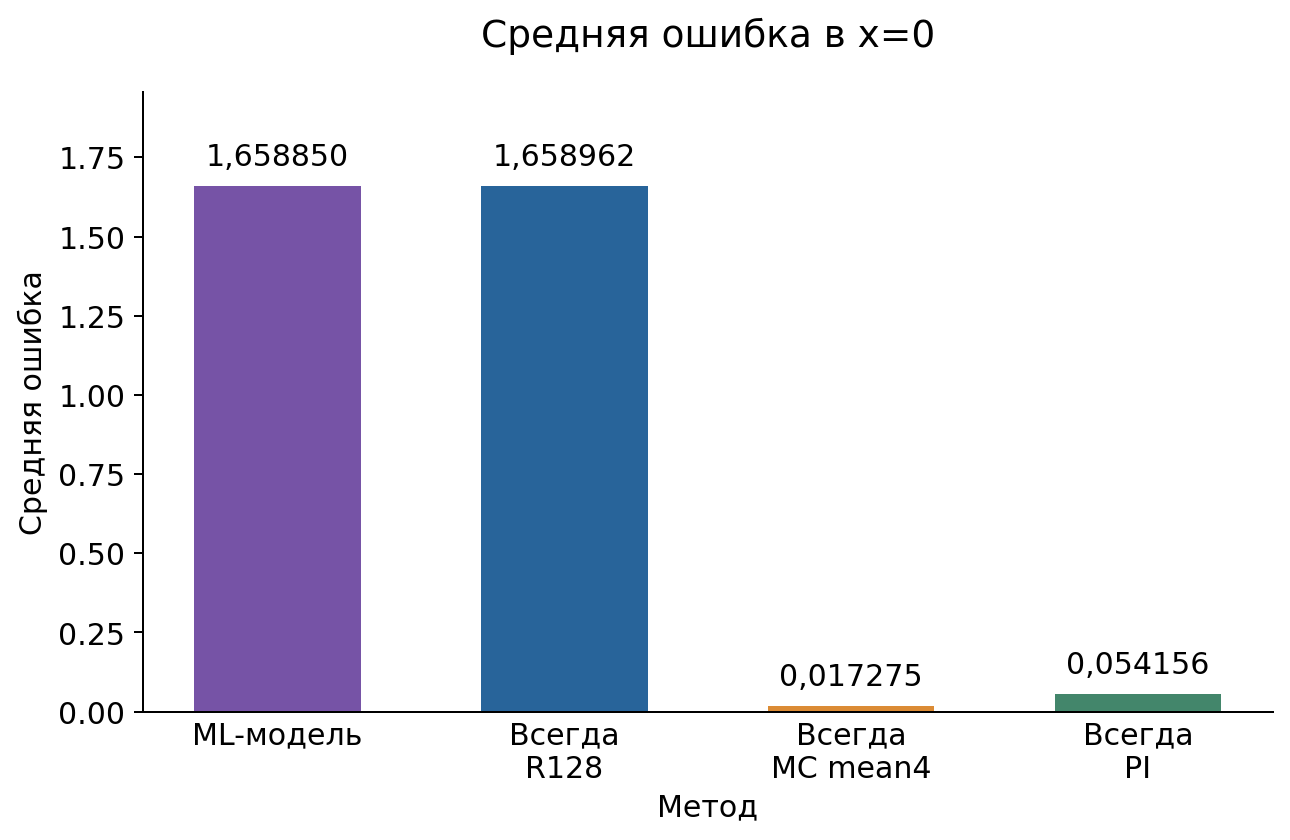
\includegraphics[width=0.85\textwidth]{04_mean_error.png}
\caption{Средняя ошибка выбранного метода в точке $x=0$ на тестовой
выборке для модели и для постоянного выбора одного метода. R128 ---
метод Ремизова, MC mean4 --- Монте-Карло, PI --- мультипликативный
интеграл.}
\label{fig:ml3-mean}
\end{figure}

На рис.~\ref{fig:ml3-imp} показаны пять признаков с наибольшей
важностью. Важность --- внутренняя оценка CatBoost вклада признака
в изменение предсказаний; сумма важностей всех 258 признаков равна 100\%.
Наиболее важны среднеквадратичное значение $b$ (10.36\%; приложение,
П.2, величина 5), значение $b$ в узле $x\approx0.545$ (5.15\%; П.1),
число $\lambda$ (4.85\%; П.5), полная вариация коэффициента $a$
(4.62\%; П.2, величина 8) и величина $\sqrt{2A_+T}$ (4.27\%; П.6,
величина 7). Вместе на них приходится около 29\% суммарной важности.
Важность показывает, какими признаками модель пользуется больше всего,
но не объясняет, почему один метод точнее другого.

\begin{figure}[!htbp]
\centering
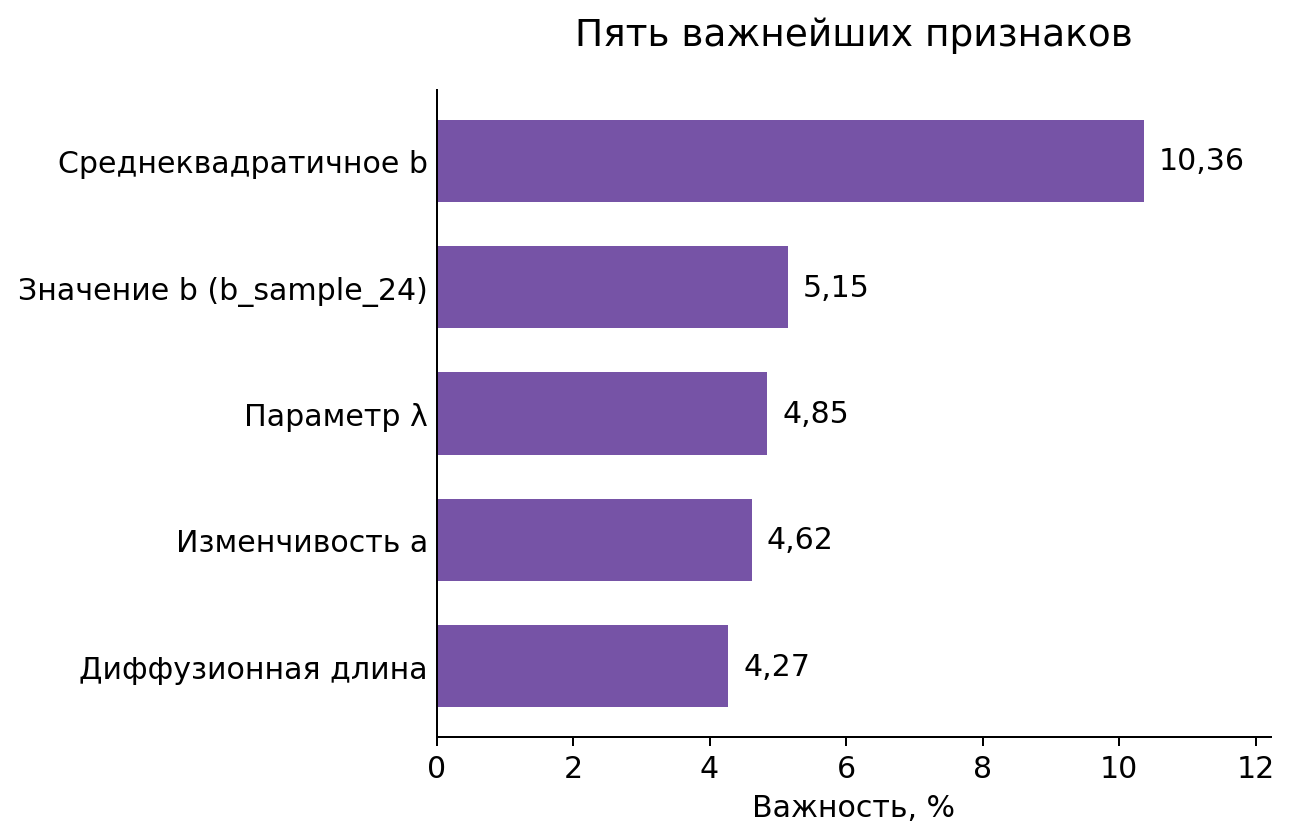
\includegraphics[width=0.85\textwidth]{06_top5_features.png}
\caption{Пять признаков с наибольшей важностью в модели выбора из трёх
методов. <<Значение b (b\_sample\_24)>> --- значение $b$ в узле
$x\approx0.545$; <<Диффузионная длина>> --- величина $\sqrt{2A_+T}$.}
\label{fig:ml3-imp}
\end{figure}

Таким образом, построен и проверен полный процесс автоматического выбора
одного из трёх методов по признакам уравнения, но на тестовой выборке
модель не лучше постоянного выбора метода Ремизова: доля верных выборов
у неё на 2 процентных пункта меньше, а число уравнений с достигнутой
точностью и средняя ошибка практически те же. Результат относится
к фиксированным настройкам методов и к ошибке в точке $x=0$; тестовая
выборка ранее использовалась в других расчётах проекта, поэтому оценка
не является полностью независимой.

\section{Заключение}
\subsection{Краткие выводы по полученным результатам}
\begin{enumerate}
\item Построен набор из 1000 уравнений с известными точными решениями,
в котором коэффициент $a$ положителен и $\lambda>\sup_x|c(x)|$
по построению, и получены ошибки четырёх численных методов в точке
$x=0$.
\item Метод Ремизова точнее Монте-Карло на 881 уравнении из 997
и достигает точности $0.05$ на 982 из них, но изредка его ошибка
на несколько порядков больше (до 842).
\item Диагностический бинарный кандидат CatBoost258 находит
6 из 9 тестовых уравнений, где точнее
Монте-Карло, но делает 14 ошибочных выборов и 3 пропуска; два ошибочных
выбора приводят к потере точности $0.05$. Его выигрыш в средней ошибке
определяется одним уравнением, поэтому устойчивого преимущества перед
постоянным выбором метода Ремизова нет. Выводы ограничены повторным
использованием тестовой выборки и малым числом уравнений, где точнее
Монте-Карло. Выбранная по Validation модель с 253 признаками
имеет на Test accuracy 91.33\%, macro-F1 0.543860 и 146 ответов
в допуске; её средняя ошибка также не лучше постоянного Ремизова.
\item Выбор более точного метода и достижение точности $0.05$ ---
разные свойства: верно выбранный метод может не достигать точности.
\item При выбранных настройках RK4 точнее остальных методов в точке
$x=0$ на всех 997 уравнениях и достигает точности $0.05$ на всех 1000,
поэтому выбор из четырёх методов на этом наборе тривиален. Это результат
для данного набора и данных настроек, а не доказательство превосходства
RK4 в общем случае.
\item Отдельная проверка максимальной ошибки на 33 узлах сохраняет
победу RK4 на всех 997 общих уравнениях. Для MC использована только
нижняя оценка через сохранённую ошибку в нуле; полного сеточного
MC-расчёта нет. Сеточный допуск выполнен у Ремизова на 970/997,
у RK4 на 1000/1000, у PI на 404/1000. Непрерывная норма не доказана.
\item Модель выбора из трёх методов --- Ремизова, Монте-Карло и метода
мультипликативного интеграла --- верно определяет лучший метод
на 88.67\% тестовых уравнений, а выбранный ею метод достигает точности $0.05$
на 98\% из них. Однако постоянный выбор метода Ремизова даёт 90.67\%
и те же 98\%: модель почти всегда выбирает метод Ремизова (146 раз
из 150) и не находит ни одного уравнения, где точнее другой метод.

\item На 60 development-задачах при $E_{33}\le0.01$ oracle выбирает
только RK4 (59 раз $N=32$, один раз $N=64$). Экономия относительно
постоянного RK4($N=64$) равна 49.1967\% в среднем по относительным
стоимостям и 48.2849\% по сумме, но дополнительный выигрыш относительно
RK4-only выбора $N$ равен нулю. Для ML выбора метода получено NO-GO.
\item В граничной development-проверке все три исходные $E_{33}>1$
устранены, контролей в допуске осталось 30/30, проблемных стало
1/22 вместо 0/22. Формальный NO-GO вызван тремя увеличениями
порядка $10^{-9}$ сверх заранее заданного строгого порога; практически
заметного ухудшения они не устанавливают. В этой серии сохраняются
21 неточный случай и теоретические ограничения пространственной схемы.
Производственный профиль не заменён.
\end{enumerate}

\subsection{Оценка полноты решения поставленных задач и планируемое развитие}
Завершён точечный эксперимент: построен набор уравнений и признаки,
получены ошибки четырёх методов в нуле, исследованы бинарные модели,
разобраны неверные выборы диагностического CatBoost258 и проверена
отдельная трёхметодная модель. По сохранённым данным дополнительно
получены ошибки R/RK4/PI на 33 узлах и обосновано сохранение победы
RK4 с использованием нижней оценки для MC. Отдельно завершены
ограниченный cost60-пилот и граничная development-проверка; их результаты
приведены в разделах~\ref{sec:costpilot} и~\ref{sec:boundarydev}.
При подготовке настоящей сводной редакции использовались только
сохранённые результаты: новых solver-, MC-, fit- и inference-вызовов нет.
Ранее выполненные численные серии не смешиваются с редакторской проверкой.

Открытыми остаются следующие вопросы:
\begin{enumerate}
\item Полная сеточная ошибка MC, её статистический разброс и смещение
временной дискретизации; оценка ML-моделей по сеточной цели.
\item Ошибка между контрольными узлами и контролируемые серии
уточнения. Стоимость достижения допуска за пределами выполненного
пилота, включая стоимость выбора/пробных решений, не установлена.
\item Пространственная устойчивость Ремизова, строгий контроль окна
и разделение остаточной ошибки после zero-проверки; причины трёх
исторических выходов worker остаются неизвестными.
\item Переносимость селектора на новые семейства и сравнение методов
при явно согласованной доступности начальных данных. Исторический
Test не является новым независимым подтверждением.
\end{enumerate}
Эти вопросы не заменяют полученные результаты, но ограничивают
их интерпретацию. Увеличение сложности ML и генерация новых уравнений
без отдельной проверяемой гипотезы из текущих данных не следуют.

\clearpage
\renewcommand{\refname}{Список использованных источников}
\phantomsection
\addcontentsline{toc}{section}{Список использованных источников}
\begin{thebibliography}{9}
\raggedright
\bibitem{repo2488} Timofeev, M. Yu.. ode-generator-remizov: генератор уравнений, решатели и эксперименты по выбору метода. GitHub. 2026. URL: \url{https://github.com/MikTi05/ode-generator-remizov}.

\bibitem{savedgrid} Сохранённые результаты проекта: серия Ремизова
\path{results/chernov_solve1000_2026-10-18/solutions/};
траектории RK4 и PI в
\path{results/four_method_accuracy_1000_2026-11-01/records/};
MC-ответы в нуле в \path{results/mc1000_x0_2026-10-25/attempts/}.
Проверка 997 общих уравнений без новых решений:
\path{results/scientific_report_revision_2026-11-04/grid33_verification.json}
и \path{results/scientific_report_revision_2026-11-04/grid33_per_equation.csv}.
Самодостаточная новая таблица и её проверка приведены в источнике~\cite{savedgrid33release}.
\bibitem{savedmodels} Сохранённый выбор бинарной модели:
\path{results/ml_selector_hypotheses_2026-10-31/selection_lock.json};
проверенные метрики в
\path{results/scientific_evidence_2026-11-01/tables/main_model_comparisons.csv}.
\bibitem{savedboundary} Сохранённая диагностика граничного продолжения:
\path{results/chernov_boundary_diagnosis_2026-10-24/REPORT.md}.

\bibitem{savedgrid33release} Проверенные сеточные результаты проекта:
\path{results/saved_grid33_1000_2026-11-04/}.
В комплекте этой редакции: \path{evidence/grid33/grid33_all1000.csv},
\path{evidence/grid33/summary.json}, \path{evidence/grid33/verification.json}.
\bibitem{savedgrid33figures} Научное оформление сохранённых E33:
\path{results/grid33_scientific_presentation_2026-11-04/}.
Исходные данные рисунков и таблиц: \path{evidence/grid33_figures/figure_data.json},
\path{evidence/grid33_figures/comparison.csv}; изображения сохранены побайтово.
\bibitem{savedcost60} Ограниченный development-пилот стоимости RK4/PI:
\path{results/cost60_rk4_pi_2026-11-04_v2/}.
План, профили, winner-таблица и независимая проверка:
\path{evidence/cost60/plan.json}, \path{evidence/cost60/profiles.csv},
\path{evidence/cost60/winners.csv}, \path{evidence/cost60/verification.json}.
\bibitem{savedboundarydev} Development-проверка граничного продолжения:
\path{results/remizov_boundary_dev_2026-11-05/}.
Таблица до/после и регрессии:
\path{evidence/boundary_dev/before_after.csv},
\path{evidence/boundary_dev/material_regressions.csv}; пространственный разбор:
\path{evidence/boundary_dev/SPATIAL_ASSESSMENT.md}.
\bibitem{savedthreeML} Проверенные результаты трёхметодного ML-селектора:
\path{results/ml_three_method_selector_2026-11-03/}.
Сохранённые Test-метрики и независимая сверка:
\path{evidence/ml_three/test_metrics.json}, \path{evidence/ml_three/verification.json}.
\end{thebibliography}

\clearpage
\section*{Приложение. Признаки модели выбора метода}
\phantomsection
\addcontentsline{toc}{section}{Приложение. Признаки модели выбора метода}

Признаки вычисляются по функциям $v\in\{a,b,c,g\}$ из
уравнения~\eqref{eq:ode} на сетке $x_i=-1+2i/255$, $i=0,\dots,255$;
$v_i=v(x_i)$. Всего признаков
\[
258=128+56+6+48+5+10+5.
\]

\subsection*{П.1. Значения функций (128 признаков)}
Для каждой функции $v\in\{a,b,c,g\}$ берутся 32 значения
\[
v\bigl(x_{j_k}\bigr),\qquad j_k=\lfloor 255k/31\rfloor,\quad k=0,\dots,31,
\]
то есть значения в почти равноотстоящих узлах от $x=-1$ до $x=1$.
Значения берутся в узлах сетки, без интерполяции.

\subsection*{П.2. Статистики функций (56 признаков)}
Для каждой функции $v\in\{a,b,c,g\}$ вычисляются 14 величин из
таблицы~\ref{tab:app-stats}. Обозначения:
\begin{gather*}
\bar v=\frac1{256}\sum_{i=0}^{255}v_i,\qquad
d^{(1)}_i=\frac{v_{i+1}-v_i}{x_{i+1}-x_i},\quad i=0,\dots,254,\\
d^{(2)}_i=\frac{d^{(1)}_{i+1}-d^{(1)}_i}{m_{i+1}-m_i},\quad i=0,\dots,253,
\end{gather*}
где $m_i=(x_i+x_{i+1})/2$ --- середины отрезков сетки;
$d^{(1)}$ и $d^{(2)}$ --- разностные оценки первой и второй производных.
Через $\hat v_k$ обозначено дискретное преобразование Фурье
последовательности $v_i-\bar v$, $P_k=|\hat v_k|^2$, $k=0,\dots,128$.

\begin{table}[!htbp]
\centering
\caption{Статистики, вычисляемые для каждой из функций $a,b,c,g$.}
\label{tab:app-stats}
\renewcommand{\arraystretch}{1.25}
\begin{tabular}{r>{\raggedright\arraybackslash}p{0.4\textwidth}l}
\toprule
№ & Величина & Формула\\
\midrule
1 & максимум & $\max_i v_i$\\
2 & минимум & $\min_i v_i$\\
3 & среднее & $\bar v$\\
4 & стандартное отклонение & $\Bigl(\frac1{256}\sum_i(v_i-\bar v)^2\Bigr)^{1/2}$\\
5 & среднеквадратичное значение & $\Bigl(\frac1{256}\sum_i v_i^2\Bigr)^{1/2}$\\
6 & максимум модуля & $\max_i|v_i|$\\
7 & медиана & медиана чисел $v_0,\dots,v_{255}$\\
8 & полная вариация & $\sum_{i=0}^{254}|v_{i+1}-v_i|$\\
9 & среднеквадратичная первая производная & $\Bigl(\frac1{255}\sum_i\bigl(d^{(1)}_i\bigr)^2\Bigr)^{1/2}$\\
10 & максимум модуля первой производной & $\max_i\bigl|d^{(1)}_i\bigr|$\\
11 & среднеквадратичная вторая производная & $\Bigl(\frac1{254}\sum_i\bigl(d^{(2)}_i\bigr)^2\Bigr)^{1/2}$\\
12 & доля отрицательных значений & $\frac1{256}\,\#\{i:\ v_i<0\}$\\
13 & число смен знака & $\#\{i:\ v_iv_{i+1}<0\}$\\
14 & доля высоких частот & $\sum_{k\ge8}P_k\big/\sum_kP_k$\\
\bottomrule
\end{tabular}
\end{table}
Если $\sum_kP_k=0$ (функция постоянна), величина 14 полагается равной нулю.

\subsection*{П.3. Корреляции (6 признаков)}
Для каждой пары функций $(a,b)$, $(a,c)$, $(a,g)$, $(b,c)$, $(b,g)$,
$(c,g)$ вычисляется коэффициент корреляции значений на сетке
\[
\rho(v,w)=\frac{\sum_i(v_i-\bar v)(w_i-\bar w)}
{\sqrt{\sum_i(v_i-\bar v)^2}\,\sqrt{\sum_i(w_i-\bar w)^2}};
\]
если одна из функций постоянна, полагается $\rho=0$.

\subsection*{П.4. Характеристики формул коэффициентов (48 признаков)}
Формулы $T_a,T_b,T_c$ из~\eqref{eq:ml-coef} записываются в виде дерева
операций (до преобразования $\tanh$). Для каждой из трёх формул
вычисляются 16 величин: общее число узлов дерева, глубина дерева
(корень имеет глубину 1) и число узлов каждого из 14 видов
из таблицы~\ref{tab:app-ops}. Числовые параметры $\alpha,\beta,\omega,
\varphi,\mu$ в признаки не входят. Формула точного решения не используется.

\begin{table}[!htbp]
\centering
\caption{Виды узлов в формулах коэффициентов.}
\label{tab:app-ops}
\renewcommand{\arraystretch}{1.3}
\begin{tabular}{>{\raggedright\arraybackslash}p{0.32\textwidth}l}
\toprule
Тип узла & Вид\\
\midrule
функции от $x$ (листья) & константа;\ $\sin(\omega x+\varphi)$;\ $\cos(\omega x+\varphi)$;\\
 & $\tanh(\omega x+\varphi)$;\ $e^{-\alpha(x-\mu)^2}$;\\
 & $\dfrac{1}{1+\alpha(x-\mu)^2}$;\ $\dfrac{x-\mu}{\sqrt{1+(x-\mu)^2}}$\\
\midrule
функции одного аргумента $u$ & $\sin u$;\ $\cos u$;\ $\tanh u$;\ $e^{-u^2}$;\ $\dfrac{u}{1+u^2}$\\
\midrule
функции двух аргументов $u,w$ & $\alpha u+\beta w$;\ $u\cdot w$\\
\bottomrule
\end{tabular}
\end{table}

Для гауссовского и лоренцевского листьев параметр $\alpha>0$.

\subsection*{П.5. Границы коэффициентов (5 признаков)}
Числа $A_-$, $A_+$, $B$, $C$ и $\lambda$ из~\eqref{eq:ml-coef}:
\[
A_-\le a(x)\le A_+,\qquad |b(x)|\le B,\qquad |c(x)|\le C
\quad\text{при всех } x\in\mathbb R.
\]
Это гарантированные аналитические границы, следующие из формул
коэффициентов; они не обязаны быть наилучшими и не являются
минимумами и максимумами значений на контрольной сетке.

\subsection*{П.6. Величины, вычисляемые по границам (10 признаков)}
Величины из таблицы~\ref{tab:app-derived} вычисляются по границам
из раздела П.5. Здесь $T$ --- верхний предел интеграла по $t$ в методе
Ремизова (раздел~\ref{sec:ml-methods}) при $\varepsilon_T=10^{-8}$,
а $\tau=T/n$ при $n=128$ --- наибольший шаг в операторе $S(\tau)$.

\begin{table}[!htbp]
\centering
\caption{Величины, вычисляемые по границам коэффициентов.}
\label{tab:app-derived}
\renewcommand{\arraystretch}{1.25}
\begin{tabular}{rl>{\raggedright\arraybackslash}p{0.46\textwidth}}
\toprule
№ & Формула & Смысл\\
\midrule
1 & $\delta=\lambda-C$ & запас в условии $\lambda>\sup_x|c(x)|$\\
2 & $T=\max\Bigl(0,\ \dfrac1\delta\ln\dfrac{2}{\delta\cdot10^{-8}}\Bigr)$ & верхний предел интеграла по $t$\\[8pt]
3 & $T/128$ & наибольший шаг $\tau$ в операторе $S(\tau)$\\
4 & $\lambda T$ & параметр затухания множителя $e^{-\lambda t}$ на $[0,T]$\\
5 & $CT$ & произведение границы $|c|$ на $T$\\
6 & $A_+/A_-$ & отношение верхней и нижней аналитических границ $a$\\
7 & $\sqrt{2A_+T}$ & характерный масштаб сдвигов, связанных с $a$, за время $T$\\
8 & $2\sqrt{A_+T/128}$ & верхняя граница модуля диффузионного сдвига в $S(\tau)$\\
9 & $BT$ & характерный масштаб сдвигов, связанных с $b$, за время $T$\\
10 & $2BT/128$ & верхняя граница модуля дрейфового сдвига в $S(\tau)$\\
\bottomrule
\end{tabular}
\end{table}

\subsection*{П.7. Отношения слагаемых уравнения (5 признаков)}
Положим $q(x)=\lambda-c(x)>0$; $a_0,b_0,q_0$ --- значения $a,b,q$ в точке
$x=0$, найденные линейной интерполяцией по сетке. Производные вычисляются
разностными формулами второго порядка на той же сетке, интегралы ---
по формуле трапеций на $[-1,1]$; $\operatorname{RMS}(u)=
\bigl(\frac1{256}\sum_iu_i^2\bigr)^{1/2}$.

Если в уравнении~\eqref{eq:ode} пренебречь слагаемыми $af''$ и $bf'$,
то получается простое приближение $f\approx u=g/q$. Признаки сравнивают
величины слагаемых уравнения и показывают, насколько это приближение
нарушается.

\begin{table}[!htbp]
\centering
\caption{Отношения слагаемых уравнения.}
\label{tab:app-extra}
\renewcommand{\arraystretch}{1.6}
\begin{tabular}{rl>{\raggedright\arraybackslash}p{0.46\textwidth}}
\toprule
№ & Формула & Смысл\\
\midrule
1 & $\dfrac{|b_0|}{\sqrt{a_0q_0}}$ & величина коэффициента $b$ по сравнению с $a$ и $q$ в нуле\\[10pt]
2 & $\dfrac{a_0\,\operatorname{RMS}(g'')}{q_0\,\operatorname{RMS}(g)}$ & величина $ag''$ по сравнению с $qg$\\[10pt]
3 & $\dfrac{\operatorname{RMS}(a')}{\sqrt{a_0q_0}}$ & изменчивость коэффициента $a$\\[10pt]
4 & $\dfrac{\bigl|\int_{-1}^{1}g\,dx\bigr|}{\int_{-1}^{1}|g|\,dx}$ & взаимное погашение положительной и отрицательной частей $g$\\[10pt]
5 & $\dfrac{\operatorname{RMS}(au''+bu')}{\operatorname{RMS}(g)},\ u=g/q$ & невязка приближения $f\approx g/q$ в уравнении\\
\bottomrule
\end{tabular}
\end{table}
При $g\equiv0$ признаки 2, 4 и 5 полагаются равными нулю.
\end{document}